\documentclass[12pt,a4paper,twoside]{book}

% use Libertine font
\usepackage{libertine}
\usepackage{inconsolata}
\usepackage[T1]{fontenc}

\usepackage[utf8]{inputenc}
\usepackage[inline]{enumitem}
\usepackage{parskip} % disable indentation for new paragraphs, increased margin-bottom instead
\usepackage[ngerman,american]{babel}
\usepackage{csquotes}

\usepackage{kit_style/kitthesiscover}

\usepackage[style=alphabetic,backend=biber]{biblatex}
\addbibresource{bib.bib}
\addbibresource{bib_manual.bib}
\setcounter{biburlnumpenalty}{100}
\setcounter{biburllcpenalty}{7000}
\setcounter{biburlucpenalty}{8000}

\usepackage{todonotes}
\usepackage{blindtext}

\usepackage{xparse}

\usepackage{xspace}

\usepackage{listings}

\usepackage{float} % for the [H] option on figures

% for core allocation pseudo-code mostly...
\usepackage{amsmath}
\usepackage{algorithmicx}
\usepackage{varwidth}
\usepackage{calc} % for \widthof
%\usepackage{algorithm}
\usepackage{algpseudocode}
\usepackage{mathtools}
\DeclarePairedDelimiter\ceil{\lceil}{\rceil}
\DeclarePairedDelimiter\floor{\lfloor}{\rfloor}
\usepackage{amsfonts}
\usepackage{setspace}

% pandas to_latex tables look good this way
\usepackage{booktabs}
\usepackage{multirow}

\usepackage{subcaption}

\usepackage{placeins}

\usepackage{hyperref}

\usepackage{siunitx}

% listings style
\lstdefinestyle{figurec}{
  belowcaptionskip=1\baselineskip,
  language=C,
  basicstyle=\footnotesize\ttfamily,
  frame=single,
  xleftmargin=\parindent,
  alsodigit={:},
  tabsize=4,
}
\lstdefinestyle{figurepseudocode}{
%   belowcaptionskip=1\baselineskip,
  belowskip=0pt,
  showstringspaces=false,
  language=C,
  basicstyle=\footnotesize\ttfamily,
  frame=single,
  xleftmargin=\parindent,
  alsodigit={:},
  tabsize=4,
}
%% set default style
\lstset{style=figurec}


% custom commands
\newcommand{\impl}[0]{$\Rightarrow$}

\widowpenalty100000
\clubpenalty100000
\raggedbottom

\begin{document}
\frontmatter
\unitlength1cm
\selectlanguage{american}

\title{Low-Latency Synchronous I/O For OpenZFS Using Persistent Memory}
\author{Christian Schwarz}
\thesistype{ma}
\primaryreviewer{Prof.\ Dr.\ Frank Bellosa}
\advisor{Lukas Werling, M.\ Sc.}{}
\thesisbegindate{TODO}
\thesisenddate{TODO}
\maketitle

\thispagestyle{empty}
\vspace*{30\baselineskip}
%\hbox to \textwidth{\hrulefill}
\par
\iflanguage{ngerman}{
\noindent Ich versichere wahrheitsgem"a"s, die Arbeit selbstst"andig verfasst, alle benutzten Hilfsmittel vollst"andig und genau angegeben und alles kenntlich gemacht zu haben, was aus Arbeiten anderer unver"andert oder mit Ab"anderungen entnommen wurde sowie die Satzung des KIT zur Sicherung guter wissenschaftlicher Praxis in der jeweils g"ultigen Fassung beachtet zu haben.\\

\noindent Karlsruhe, den \declaration@date
}{
\noindent I hereby declare that the work presented in this thesis is entirely my own and that I did not use any source or auxiliary means other than these referenced. This thesis was carried out in accordance with the Rules for Safeguarding Good Scientific Practice at Karlsruhe Institute of Technology (KIT).\\

\noindent Karlsruhe, \declaration@date
}

%%%%%%%%%%%%%%%%%%%%%%%%%%%%%%%%%%%%%%%%%%%%%%%%%%%%%%%%%%%%%%%%%%%%%%%%
%% Hinweis:
%%
%% Diese Erklärung wird von der Prüfungsordnung für Diplomarbeiten 
%% verlangt und ist zu unterschreiben. Für Studienarbeiten ist diese
%% Erklärung nicht zwingend notwendig, schadet aber auch nicht.
%%%%%%%%%%%%%%%%%%%%%%%%%%%%%%%%%%%%%%%%%%%%%%%%%%%%%%%%%%%%%%%%%%%%%%%%
\clearpage








\chapter{Abstract}
\blindtext

\mainmatter
\cleardoublepage
\phantomsection
\addcontentsline{toc}{chapter}{Contents}
\tableofcontents

\chapter{Introduction}
The task of a filesystem is to provide non-volatile storage to applications in the form of the \textit{file} abstraction.
Applications modify files through system calls such as \lstinline{write()} which generally does not provide any durability guarantees.
Instead, the system call modifies a buffer in DRAM such as a page in the Linux page cache and returns to userspace.
Synchronization of the dirty in-DRAM data to persistent storage is thus deferred to a --- generally implementation-defined --- point in the future.

However, many applications have more specific durability requirements.
For example, an accounting system that processes a purchase needs to ensure that the updated account balance is persisted to non-volatile storage before clearing the transaction.
Otherwise, a system crash and recovery after clearing could result in the pre-purchase balance being restored, enabling double-spending by the account holder.
These \textbf{synchronous I/O} semantics must be requested through APIs auch as \lstinline{fsync()} which "assure that after a system crash [...] all data up to the time of the \lstinline{fsync()} call is recorded on the disk."~\cite{posix_fsync_opengroup}.

The \textbf{Zettabyte File System (ZFS)} is a combined volume manager and filesystem.
It pools many block devices into a single storage pool (\textit{zpool}) which can hold thousands of sparsely allocated filesystems.
The ZFS on-disk format is a merkle tree that is rooted in the \textit{uberblock} which is ZFS's equivalent of a superblock.
ZFS on-disk state is always consistent and moves forward in so-called \textit{transaction groups} (txg), using copy-on-write to apply updates.
Whenever a new version of the on-disk state needs to be synced to disk, ZFS traverses its logical structure bottom up and builds a new merkle tree.
The updated parts of the tree are stored in newly allocated disk blocks while unmodified parts are re-use the existing block written in a prior txg.
Once all updates have been written out, the new uberblock is written, thereby atomically moving the on-disk format to its new state.
This procedure is called \textit{txg sync} and is triggered periodically (default: every \SI{5}{s}) or if the amount of dirty data exceeds a configurable threshold.

Synchronous I/O semantics cannot be reasonably implemented through txg sync due to the write amplification and CPU overhead inherent to the txg sync procedure.
Instead ZFS maintains the \textbf{ZFS Intent Log (ZIL)} which is a per-filesystem write-ahead log.
Unlike systems such as Linux's \textit{journaling block device 2} (JBD2), the ZIL is a logical log:
the ZIL's records describe the \textit{logical} changes that need to applied in order to achieve the state that was reported committed to userspace.
On disk, the log records are written into a chain of \textit{log-write blocks} (LWBs), each containing many records.
The LWB chain is rooted in the \textit{ZIL header} within the filesystem's representation within the merkle tree.
New LWBs are appended to the chain independently of txg sync.

By default, LWBs are allocated on\todo{from?} the zpool's main storage devices.
Consequently, the lower bound for synchronous I/O latency in ZFS is the time required to write the LWBs that contains the synchronous I/O operation's ZIL records.
For the case where this latency is insufficient, ZFS provides the ability to add a \textit{separate log device} (SLOG) to the zpool.
The SLOG is typically a single (or mirrored) block device that provides lower latency than the main pool's devices.
A typical configuration today is to add a fast NVMe drive to an HDD-based pool.
Adding a fast SLOG accelerates LWB writes because LWBs are preferentially allocated from the SLOG.
Note that SLOGs only need very limited capacity since LWBs are generally obsolete after three txgs.

\textbf{Persistent Memory (PMEM)} is an emerging storage technology that provides low-latency memory-mapped byte-addressable persistent storage.
The Linux kernel can expose PMEM as a pseudo block device whose sectors map directly to the PMEM space.
Thereby existing block devices consumers can benefit from PMEM' low latency without modification.
Block device consumers that wish to bypass block device emulation use the kernel-internal \textit{DAX} API which translates sector numbers to kernel virtual addresses, giving software \textbf{d}irect \textbf{ac}cess to PMEM.

The motivation for this thesis is to accelerate synchronous I/O in ZFS by using PMEM as a ZFS SLOG device.
A single DIMM of the current\todo{product name} Intel Optane PMEM product line can sustain 530k random 4k write IOPS which corresponds to a write latency of \SI{1.88}{us}.
However, when configuring the Linux PMEM block device as a SLOG in OpenZFS 2.0, a single thread only achieves 12k random 4k synchronous write IOPS~($\sim$~\SI{83}{us}), scaling up to 100k IOPS at 16 threads (8 cores, 2xSMT) at doubled latency.
In contrast, the same workload applied directly to the PMEM block device is able to achieve 500k IOPS with two threads~($\sim$~\SI{4}{us} per thread).
And Linux 5.9's ext4 on the PMEM block device achieves 100k random 4k write IOPS ($\sim$~\SI{}) with a single thread and scales approximately linearly to up to 466k IOPS at four threads.
\todo{review numbers in this paragraph}

Our investigation of the latency distribution for the OpenZFS PMEM SLOG configuration shows that the ZIL implementation contributes \SI{48}{us} in the single-threaded case and up to \SI{95}{us} at eight threads.
More specifically, up to \SI{50}{\%}\todo{run this again without ebpf} of total syscall latency is spent waiting for the \textit{ZIO pipeline}, excluding the time spent in the PMEM block device driver.

ZIO is ZFS's abstraction for performing IO to the pool's storage devices.
The pipeline-oriented design has proven extremely flexible and extensible over ZFS's lifetime.
Many of ZFS’s distinguishing features are implemented in ZIO, including physical block allocation, transparent data and metadata checksumming, compression, deduplication and encryption as well as redundancy mechanisms such as raidz.
CPU-intensive processing steps are parallelized to all of the system's CPUs using \textit{taskq}s.

It is our impression that ZIO is biased towards throughput, not latency.
For example, ZIO's main consumer is \textit{txg sync} which issues the updates to the on-disk merkle tree as a large tree of dependent ZIOs.
Other consumers such as periodic data integrity checking (\textit{scrubbing}) are also throughput-oriented.
In contrast, the ZIL is the only component that is latency-oriented.
ZIO's latency overhead with fast block devices such as NVMe drives is a well known problem among ZFS developers.\todo{ref, gh issue, cite private conversation with brian?}

Given
\begin{itemize}[noitemsep]
    \item the abysmal\todo{too harsh?} out-of-the-box performance of the PMEM block device as a SLOG, and
    \item our findings on\todo{right prep?} the ZIL's and ZIO pipeline's significant latency overhead, as well as the fact that
    \item grouping log records into log-write \textit{blocks} is unnecessary with byte-addressable PMEM,
\end{itemize}
we believe that the current ZIL design is fundamentally unfit to reap the performance available with PMEM.
We present \textbf{ZIL-PMEM}, a new implementation of the ZIL that bypasses the ZIO pipeline completely and persists log entries directly to PMEM.
It coexists with the existing ZIL which we refer to as \textit{ZIL-LWB} in the remainder of this document.
ZIL-PMEM achieves 140k random 4k sync write IOPS with a single thread~($\sim$~\SI{7.1}{us}) and scales up to 400k IOPS at 8 threads before it becomes CPU-bound.
This corresponds to a speedup of 6.8x (or 4x, respectively) over ZIL-LWB.\todo{review numbers}
Our implementation is extensively unit-tested and passes the ZFS test suite's SLOG integration tests.

The remainder of this thesis is structured as follows:
in Chapter 2\todo{automatic chapter numbers} we
review prior work in the field of persistent memory related to filesystems and
provide background knowledge on the integration of PMEM in the Linux kernel as well as
a detailed introduction to the components of ZFS that are relevant for this thesis.
Chapter 3 contains our performance analysis of ZIL-LWB with a PMEM SLOG, making the case for a PMEM-specific ZIL implementation.
The design and implementation of ZIL-PMEM is then presented in Chapter 4, followed by its evalation in Chapter 5.
We conclude with a summary of our findings in Chapter 6.

%In the following sections, we present
%the user experience of configuring a pool with ZIL-PMEM,
%our strategy for code-sharing between ZIL-PMEM and ZIL-LWB and
%the design of ZIL-PMEM, including
%our strategy for how we integrate PMEM log VDEVs into the vdev / zpool config layer
%ZIL-PMEM’s physical data structure,FEe
%its insertion and garbage collection algorithm,
%its claiming & replay algorithm and
%its integration into the existing OpenZFS software architecture.

\chapter{Literature Review \& Background}
In this chapter we present prior work in the field of persistent memory and its application in various storage systems developed in research and industry.
The last two sections on PMEM in Linux and ZFS provide the technical background knowledge that is necessary to understand the performance analysis of ZIL-LWB in Chapter~\ref{ch:lwb_analysis} and the design of ZIL-PMEM in Chapter~\ref{ch:di}.

\section{Literature Review}
We have surveyed publications in the area of persistent memory storage systems, filesystem guarantees \& crash-consistency models, PMEM-specific crash-consistency checkers and general methods to determine filesystem robustness in the presence of hardware failures.

\subsection{PMEM Filesystems}
In this subsection we present research filesystems that were explicitly designed for persistent memory.
ZIL-PMEM integrates into ZFS, a production filesystem that was not designed for persistent memory.
Hence we focus on techniques for crash consistency and data integrity that might be applicable to our work.

\subsubsection{In-Kernel PMEM Filesystems}\label{sec:in_kernel_pmem_filesystems}
The initial wave of publications around the use of PMEM in filesystems produced a set of systems that were implemented completely in the kernel.
\todo{we don't yet compare these systems with ZIL-PMEM. should we? Maybe in a compact section after we presented the design?}

\newcommand{\citerelwork}[2]{\textbf{#1~\cite{#2}}}

\citerelwork{BPFS}{conditBetterByteaddressablePersistent2009} is one of the earliest filesystems expressly designed for PMEM.
The filesystem layout in PMEM is inspired by WAFL~(\cite{hitzFileSystemDesign1994}) and resembles a tree of multi-level indirect pages that eventually point to data pages.
BPFS’s key contribution is the use of fine-grained atomic updates in lieu of journaling for crash consistency.
For example, updates to small metadata such as \textit{mtime} can be made using atomic operations.
For larger modifications, the authors introduce \textit{short-circuit shadow-paging}, a technique where updates are prepared in a copy of the page.
The updated page is then made visible through an update of the pointer in its parent indirect page.
The difference to regular copy-on-write is that, as soon as the update to an indirect page can be done through an atomic in-place operation, the atomic operation is used.
Updates thereby do not necessarily propagatate up to the root of the tree.

\citerelwork{PMFS}{dulloorSystemSoftwarePersistent2014} is another research filesystem that targets persistent memory.
The authors make frequent comparisons to BPFS.
The main differentiator from BPFS with regards to consistency is PMFS’s use of undo-logging for metadata updates and copy-on-write for data consistency in addition to hardware-provided atomic in-place updates.
The evaluation shows that their approach for metadata has between 24x and 38x lower overhead compared to BPFS (unit: number of bytes copied).
PMFS also introduces an efficient protection mechanism against accidental \textit{scribbles}.
Scribbles are bugs in the system that accidentally overwrite PMEM, e.g., due to incorrect address calculation or out-of-bounds access in the kernel.
By default, PMFS maps all PMEM read-only, thereby preventing accidental corruption of PMEM from code outside of PMFS.
When PMFS needs to modify PMEM, it temporarily disables interrupts and clears the processor's \lstinline{CR0.WP}, thereby allowing writes to read-only pages in kernel mode.~\cite{dulloorSystemSoftwarePersistent2014,intelSdmCr0WpFlag}

\citerelwork{NOVA}{xuNOVALogstructuredFile2016} is the most mature research PMEM filesystem.
NOVA uses per-inode logs for operations scoped to a single inode (e.g. write syscalls) and per-CPU journals for operations that affect multiple inodes.
The intended result is high scalability with regard to core count.
The per-inode log data structure is a linked list with a head and tail pointer in the inode.
NOVA leverages 8-byte atomic operations to update these pointers after it has written log entries.
While not explicitly called so by the authors it is our impression that the log is a logical redo log except for writes, which --- judging from the text --- are always logged at page granularity.
The authors explain the recovery procedure and measure its performance but do not address correctness in the evaluation.

\citerelwork{NOVA-Fortis}{xuNOVAFortisFaulttolerantNonvolatile2017} is a version of NOVA that introduces snapshots and hardening against data corruption.
Whereas snapshots are not relevant for this thesis because ZFS already provides this feature, the data corruption countermeasures are representative of the state of the art:
\begin{itemize}[noitemsep,beginpenalty=100000,midpenalty=100000]
    \item Handling of machine check exceptions (MCE) in case the hardware detects bit errors.
          This is done by using \lstinline{memcpy_mcsafe()} for all PMEM access.\todo{ref mcsafe explainer}
          %PMEM data is always buffered in DRAM before it is read.
    \item Detection of metadata corruption through CRC32 checksums.
    \item Redundancy through metadata replication. For metadata recovery, NOVA-Fortis compares checksums of the primary and replica and restores the variant with the matching checksum.
    \item Protection against localized unrecoverable data loss through RAID4-like parity.
          This feature only works while the file is not DAX-mmapped.
    \item Protection against Scribbles using \lstinline{CR0.WP} as described in the paragraph on PMFS.
\end{itemize}
The authors use a custom fault injection tool to corrupt data structures in a targeted manner and test NOVA Fortis's recovery capabilities.

\subsubsection{Hybrid PMEM filesystems}\label{sec:hybrid_pmem_file_systems}
A recurring pattern in PMEM filesystem design is to split responsibilities between kernel and userspace component in order to eliminate system call overhead.

\citerelwork{Aerie}{volosAerieFlexibleFilesystem2014} is a user-space filesystem based on the premise that
“SCM [Storage Class Memory] no longer requires the OS kernel [...].
Applications link to a file-system library that provides local access to data and communicates with a [user-space] service for coordination.
The OS kernel provides only coarse grained allocation and protection, and most functionality is distributed to client programs.
For read-only workloads, applications can access data and metadata through memory with calls to the file-system service only for coarse-grained synchronization.
When writing data, applications can modify data directly but must contact the file-system service to update metadata.”
The system uses a redo log maintained in each client program which is shipped to the filesystem service periodically or when a global lock is released.
It is our understanding that only log entries shipped to and validated by the filesystem service will be replayed.
The authors state that log entries can be lost if a client crashes before the log entries are shipped.
The evaluation does not address crash consistency or recovery at all.

\citerelwork{Strata}{kwonStrataCrossMedia2017} is a cross-media filesystem with both kernel and user-space components.
Since its distinguishing feature is the intelligent migration of data between different storage media we discuss it in the Section~\ref{sec:cross_media_storage_systems} on cross-media storage systems.

\citerelwork{SplitFS}{kadekodiSplitFSReducingSoftware2019} is a research filesystem that proposes a
“split of responsibilities between a user-space library file system and an existing kernel PM file system.
The user-space library file system handles data operations by intercepting POSIX calls, memory-mapping the underlying file, and serving the read and overwrites using processor loads and stores.
Metadata operations are handled by the kernel PM file system (ext4 DAX)”.
SplitFS uses a redo log with idempotent entries that is written from userspace.
As a performance optimization the authors use checksums and aligned start addresses to find valid log entries instead of an explicit linked list with persistent pointers.
The SplitFS evaluation of correctness is limited to a comparison of user-observable filesystem state between SplitFS and ext4 in DAX mode.
Recovery is evaluated only through the lens of recovery time (performance), not correctness.

\citerelwork{EvFS}{yoshimuraEvFSUserlevelEventDriven2019} is a
“user-level POSIX file system that directly manages NVM in user applications.
EvFS minimizes the latency by building a user-level storage stack and introducing asynchronous processing of complex file I/O with page cache and direct I/O.
[...]
EvFS leads to a 700-ns latency for 64-byte non-blocking file writes and reduces the latency for 4-Kbyte blocking file I/O by 20 us compared to a kernel file system [EXT4] with journaling disabled.“
In contrast to Aerie, EvFS does not require a coordinating user-space service.
Crash consistency and recovery is not addressed:
“EvFS is not a production-ready file system because it neither provides all the POSIX APIs or crash-safe properties”.

\subsection{Cross-Media Systems}\label{sec:cross_media_storage_systems}
Cross-media storage systems combine the advantages of multiple storage devices from different levels of the storage hierarchy.
Historically, these kinds of systems strive to exploit hard disk for high capacity at low cost and more expensive flash storage for low latency random access IO.
With persistent memory, a new class of storage has become available whose role in cross-media systems is still to be determined.
In the context of this thesis we find it most useful to compare the overall system architecture.

\citerelwork{ZFS: Allocation Classes}{openzfsAllocationClasses}
Whereas ZFS was initially designed for a large pool of hard disks, it has gained several cross-media features over its lifetime.
When configuring a zpool, the administrator assigns the block device to an \textit{allocation class}.
The following allocation classes exist: \textit{normal} (main pool), \textit{log} (SLOG device), \textit{aux} (L2ARC, a victim cache for ZFS's ARC\todo{check that we have explained ARC already}), \textit{special} (small blocks), and \textit{dedup} (deduplication table data).
When a function in ZFS allocates a block in the pool, it must specify the desired allocation class.
If the allocation succeeds, the allocated block is guaranteed to be located on device(s) within that class.
The use case for allocation classes is to combine the advantages of different storage media in a single pool.
In many setups devices in the \textit{normal} class have high capacity and are grouped in storage-efficient redundancy configurations such as \textit{raidz} or \textit{draid}.
A \textit{log} or \textit{aux} device can be added to a pool in order to accelerate latency-sensitive I/O such as ZIL writes.
Many administrators configure lower redundancy for these devices --- either to gain performance or to reduce costs --- which, depending on business requirements, may be justified due to the short-lived nature of ZIL writes.
In comparison to the other systems presented in this section, allocation classes are very inflexible:
once an allocation is made and the data is written, the data stays in that place until it is freed or the device is removed from the pool.
In particular, there is no automatic tiering that takes usage patterns into account.
Further, L2ARC devices reduce space efficiency because the cached data still occupies space in the main pool.
Similarly, SLOG devices are somewhat wasteful since they are exclusively used for ZIL logging and never read except during recovery.
Systems such as Strata derives more value from its PMEM-based log.
Finally, it should be noted that while Linux's /dev/pmem\todo{ref backwards} block device can be used with allocation classes, ZFS's ZIO pipeline is unable to exploit its write performance.\todo{ref section on ZIL-LWB perf}.
%On the write path, separate log devices (SLOG) can be added to a storage pool to be used exclusively for persisting ZFS’s logical write-ahead log (the ZIL).
%Offloading latency-sensitive IO to the log device allows for greater throughput during txg sync to the main pool’s devices.
%\todo{if we move the related work section to the end of the thesis this paragraph can be abbreviated}
%On the read path, the in-DRAM ARC, which is ZFS’s variant of the buffer cache, can be extended with a second-level victim cache on a block device, the L2ARC.
%L2ARC hits free up IOPS among the main pool’s devices which can be used for txg sync.

\citerelwork{ZFS: ZIL Performance Improvements For Fast Media}{openzfsZILPerformanceImprovements2020}
At the OpenZFS 2020 Developer summit, Saji Nair of storage vendor Nutanix presented a ZIL prototype that handles fast block devices more efficiently.
The prototype avoids unnecessary sequential ordering of I/O operations when writing ZIL LWBs\todo{check that LWBs have been introduced by now}.
It also avoids using the ZIO pipeline due to context switching overheads, issuing block I/O directly from the application thread instead.
The evaluation is limited to 4k sync write performance, claiming an up 4x improvement in IOPS with four threads.
However, the source code for the prototype has not been published and the design is incomplete with regards to replay.
\todo{maybe this entire section should move to the 'background' section?}

\citerelwork{Strata}{kwonStrataCrossMedia2017} is a cross-media research filesystem.
“Closest to the application, Strata’s user library synchronously logs process-private updates in NVM while reading from shared, read-optimized, kernel-maintained data and metadata.
    [...]
Client code uses the POSIX API, but Strata’s synchronous updates obviate the need for any sync-related system calls”.
We classify Strata as a hybrid filesystem in Section~\ref{sec:hybrid_pmem_file_systems} because it consists of both a userspace library and an in-kernel component.
The log, written from userspace, is an idempotent logical redo log.
The kernel component then \textit{digests} the logs asynchronously, performing aggregation of the logged operations during digestion.
Aggregation permits the kernel component to issue “sequential, aligned writes” to the slower storage devices such as SSDs or HDDs.
ZFS with and without ZIL-PMEM compares to Strata in the following ways:
\begin{itemize}[noitemsep,beginpenalty=100000,midpenalty=100000]
    \item Both systems use a logical redo operation log instead of a block-level journaling mechanism.
    \item Both systems perform asynchronous write-back and thereby reap similar benefits from it (parallel batch processing, optimized allocation).
    \item Strata’s kernel component digests the logs written from user-space in order to write them back to other tiers.
          ZFS accumulates the write-back state in DRAM and never reads the log except for recovery.
          (It is unclear to us how often Strata digests the logs. ZFS performs write-back of dirty state after at most 5 seconds.)
          % \item The Strata paper suggests that the system uses a single block size whereas ZFS supports variable block sizes (“Free Block Bitmap” in Strata vs. Spacemaps in ZFS).
    \item Strata seems to tune allocations for SSDs, e.g. allocating blocks in erasure block size to prevent write amplification.
          ZFS supports TRIM and supports variable block sizes up to \SI{16}{MiB}, but there are no automatic optimizations that specifically target write amplification in SSDs.
          %\item ZFS guarantees data integrity and has provisions for redundancy.
          %\item ZFS supports many devices at different performance class levels whereas Strata only supports a single device.
    \item ZFS is in-kernel and requires no modifications to applications whereas Strata requires linking to or LD\_PRELOADing a user-space library, which, tangentially, makes it incompatible with statically linked binaries.
          %\item ZFS is a mature filesystem used at large scale in production whereas Strata is an unproven research prototype.
\end{itemize}

\citerelwork{Ziggurat}{zhengZigguratTieredFile2019}
“Ziggurat exploits the benefits of NVMM through intelligent data placement during file writes and data migration.
Ziggurat includes two placement predictors that analyze the file write sequences and predict whether the incoming writes are both large and stable, and whether updates to the file are likely to be synchronous.
Ziggurat then steers the incoming writes to the most suitable tier based on the prediction: writes to synchronously-updated files go to the NVMM tier to minimize the synchronization overhead.
Small, random writes also go to the NVMM tier to fully avoid random writes to disk. The remaining large sequential writes to asynchronously-updated files go to disk”.
The authors compare Ziggurat to Strata as follows:
“Strata is a multi-tiered user-space file system that exploits NVMM as the high-performance tier, and SSD/HDD as the lower tiers.
It uses the byte-addressability of NVMM to coalesce logs and migrate them to lower tiers to minimize write amplification.
File data can only be allocated in NVMM in Strata, and they can be migrated only from a faster tier to a slower one.
The profiling granularity of Strata is a page, which increases the bookkeeping overhead and wastes the locality information of file accesses".
ZFS with and without ZIL-PMEM compares to Ziggurat as follows:
\begin{itemize}[noitemsep,beginpenalty=100000,midpenalty=100000]
    \item Ziggurat actively migrates data into PMEM based on access pattern.
          ZFS has no provisions for data migration within the pool after block allocation.
          The ZFS architecture such a feature is unlikely to be developed in the future (keyword: blockpointer rewrite).
    \item Ziggurat sends writes directly to the suitable tier based on prediction of future access patterns.
          If the access pattern is anticipated to be synchronous, Ziggurat choses the PMEM tier.
          The ZIL, and ZIL-PMEM specifically, only serves as a stop-gap between txg sync points of the main pool.
          Data is always written twice --- once to the log and once to the main pool ---, and never read from the log except during recovery.
          %(The \lstinline{WR_INDIRECT ZIL} log entry type mitigates this for large writes).
    \item Both systems are fully in-kernel and require no modifications to user-space applications.
    \item Ziggurat builds on NOVA-Fortis and thus inherits the PMEM-specific data integrity and redundancy mechanisms provided for the PMEM storage tier.
          ZIL-PMEM data integrity measures are more limited but can be expanded in the future (see Chapter~\ref{ch:di}).
    \item The Ziggurat paper does not mention data integrity measures or redundancy mechanisms for the block device layers beneath PMEM.
          Possibly, existing Linux features such as Device Mapper could be used to compensate.
          In contrast, ZIL-PMEM benefits from ZFS’s strong data integrity and redundancy mechanisms once the logged data is txg synced.\todo{ensure txg sync has already been explained}
    \item The Ziggurat design is “fast-first. It should use disks to expand the capacity of NVMM rather than using NVMM to improve the performance of disks as some previous systems have done”.
          ZIL-PMEM approaches persistent memory from the opposite direction, starting with a filesystem strongly focussed on block devices and only leveraging PMEM where appropriate.
    \item Ziggurat was not evaluated on actual persistent memory. The authors used memory on another NUMA node to simulate lower latencies.
          We evaluate ZIL-PMEM on commercially available PMEM hardware.
          %\item An examination of the Ziggurat code base shows that it only supports a single device per tier.
          %\item Ziggurat has been unmaintained since the publication. OpenZFS has a healthy community of both hobbyist and paid full-time contributors.
\end{itemize}

\citerelwork{dm-writecache}{WritecacheTargetLinux} is a new Linux Device Mapper target that synchronously persists writes to PMEM and performs asynchronous writes-back to the origin block device in the background.
Dm-writecache is relevant to ZIL-PMEM because both systems expose a PMEM-accelerated virtual block device.
For this use case, a write-back cache can be more space efficient because it only needs to store the most recent version of a block.
In contrast, ZIL-PMEM logs each block write (smallest block size for ZVOLs is 4k) separately and does not coalesce or delta-encode log entries.
ZIL-PMEM protects data integrity through checksums whereas dm-writecache fully relies on hardware error correction and detection, reported via \lstinline{memcpy_mcsafe()}.
Once ZVOL modifications are txg-synced\todo{backref} to the main pool, they benefit from ZFS's strong data redundancy mechanisms such as \textit{raidz}.
With dm-writecache, the origin block device driver must handle data redundancy if desired, e.g., though another Device Mapper target such as \textit{dm-raid}.
We compare the performance of the two implementations in Section X.Y \todo{ref block device comparison}):
dm-writecache delivers on the promise of low latency but shows significant lock contention with multiple threads, failing to saturate PMEM bandwidth and performing significantly worse than ZIL-PMEM.\todo{verify claim}

\subsection{Journaling \& Write-Ahead Logs Adapted PMEM}
The following publications use persistent memory to accelerate file system journals and write-ahead logs.

\citerelwork{Unioning of the Buffer Cache and Journaling Layers with Non-volatile Memory}{leeUnioningBufferCache2013} is an academic paper that presents a PMEM-aware buffer cache design which
“subsumes the functionality of caching and [block-level] journaling”.
From the buffer cache’s perspective, the on-disk blocks that make up a journal (e.g. one managed by JBD2) are indistinguishable from non-journal filesystem blocks.
Thus, for a journal block $A’$ that logs an update to a block $A$, both blocks $A’$ and $A$ will sit in the buffer cache.
This waste of space can be reduced with PMEM by the author’s proposal.
Instead of journaling on top of the block layer, one journals in the buffer cache itself by a) placing the buffer cache in PMEM and b) introducing a new buffer cache entry state “frozen” so that an entry can be “clean”, “dirty” or “frozen”.
When modifying a block $A$, the filesystem no longer makes a journal entry but instead modifies the buffer cache entry directly.
If the entry was “clean”, it is now “dirty”. If the entry was “frozen”, a copy is made and the modification goes to the copy, making it “dirty” as well.
Committing a block to the journal is a simple state transition from “dirty” to “frozen”. On a crash + restart, “dirty” buffer cache entries are discarded but “frozen” entries remain.
We find the approach exceptionally interesting and innovative and can imagine an application of the idea to the ZFS ARC.
However, the system’s real-world performance is unclear (evaluation on DRAM).
Also, we see non-trivial software engineering and maintenance problems with the approach.
Finally, the paper does not address hardware error handling or data corruption concerns at all.

\citerelwork{ext4 fast commits}{FastCommitsExt4} is a feature released in Linux 5.10.
“The fast-commit journal [...] contains changes at the file level, resulting in a more compact format.
Information that can be recreated is left out, as described in the patch posting:
For example, if a new extent is added to an inode, then  corresponding updates to the inode table, the block bitmap, the group descriptor and the superblock can be derived based on just the extent information and the corresponding inode information.
    [...] Fast commits are an addition to — not a replacement of — the standard commit path; the two work together.
If fast commits cannot handle an operation, the filesystem falls back to the standard commit path.”
The cited article mentions ongoing work to use persistent memory for ext4 fast commits.
The approach is inspired by per-inode journaling as proposed by \citeauthor{parkIJournalingFinegrainedJournaling2017} in \cite{parkIJournalingFinegrainedJournaling2017}.

\textbf{Disk-oriented database management systems} often use write-ahead logs (WALs) to allow a transaction to commit before the modified pages are written back to stable storage.
However, appending to a shared WAL file has historically been a latency and scalability bottleneck which lead to amortization techniques such as \textit{commit groups} (aka \textit{group commit}) and \textit{pre-committed transactions} that batch the WAL entries of multiple committing transactions into a single physical WAL record.%
\footnote{According to \cite{dewittImplementationTechniquesMain1984} "the notion of gronp commits appears to be past of the unwritten database folklore. The System-R implementors claim to have implemented it."}
With persistent memory, the latency bottleneck no longer lies in the raw I/O but rather the coordination overhead between multiple CPU cores and sockets, prompting new distributed logging designs that avoid a central point of contention.%
~\cite{fangHighPerformanceDatabase2011,pelleyStorageManagementNVRAM2013,johnsonAetherScalableApproach2010}
ZIL-LWB\todo{ensure this term has been established by now} employs \textit{group commit} as well although the terminology is different.
It batches log records issued by independent threads for the same filesystem into the currently \textit{open} \textit{log-write block} (LWB).
Once the open LWB is full or a timeout has passed, the open LWB is written (\textit{issued}) to disk.\todo{refer to section that explains the perf problems with ZIL-LWB}
In contrast, ZIL-PMEM commits log records directly to PMEM and allows multiple cores to do so in parallel with minimal global coordination.\todo{minimal global coordination = the commit slots + semaphore}
Our evaluation shows that the design scales well on single-socket systems.
NUMA and multi-socket systems, which are addressed in the cited publications from the database community, have been explicitly out of scope for this thesis.\todo{meh, ref}

\subsection{Testing Filesystem Crash Consistency}
In this section we survey techniques to determine and verify crash consistency guarantees of file systems.
A formal and automatically verifiable model would have been been extremely helpful to ensure that ZIL-PMEM maintains the same crash consistency guarantees as ZIL-LWB.\todo{ref}

\citerelwork{All File Systems Are Not Created Equal}{pillaiAllFileSystems2014} contributes a survey of the atomicity and ordering guarantees of several popular Linux filesystems and provides a tool called ALICE to validate or derive the guarantees required by applications.
ZFS with and without ZIL-PMEM could benefit from this survey as well.
The survey could be used to characterize ZFS’s guarantees.
ALICE could be used to determine whether ZFS’s guarantees are sufficient for applications and/or whether ZFS’s guarantees exceed the requirements of the majority of applications.
However, since ZIL-PMEM shall maintain the same guarantees as ZIL-PMEM (see Section~\ref{sec:requirements}), such findings would only be relevant for future work.

\citerelwork{Specifying and Checking File System Crash-Consistency Models}{bornholtSpecifyingCheckingFile2016}
The authors
“present a formal framework for developing crash-consistency models, and a toolkit, called FERRITE, for validating those models against real file system implementations.”
The system provides means to express expected filesystem behavior as a \textit{litmus test}.
A litmus test encodes expected behavior of a filesystem though a series of events (e.g. write to a file) and a final predicate expressed as a satisfiability problem.
FERRITE can execute the litmus test against an axiomatic formal model of the filesystem to ensure that, iff the actual filesystem adheres to the formal model, the litmus test’s expectations hold.
Notably the litmus test is executed symbolically and the validation predicates are checked for satisfiability by an SMT solver; this is exhaustive and not comparable to a unit  or regression test.
FERRITE can also execute litmus tests against the actual filesystem to test whether it adheres to the formal model.
This test is non-exhaustive.
It is based on executing the litmus test “many times” where for each execution all disk commands emitted during execution are recorded.
All permutations and prefixes of these traces that are allowed under the semantics of the disk protocol are used to produce test disk images which are fed back to the filesystem under test for recovery.
After recovery the litmus test’s predicate must hold against the concrete filesystem state after recovery.
If it does not hold the given permutation of the trace is proof that the filesystem does not match its model (assuming the litmus test passes execution against the model), or that the filesystem’s assumptions about the disk do not match the FERRITE \textit{disk model}.
FERRITE appears to be a useful tool to build a model of ZFS’s undocumented crash-consistency guarantees (ZFS has not been evaluated by the authors).
Such a model would be helpful to validate ZIL-PMEM's goal to maintain the same semantics as ZIL-PMEM.
However, this would require a FERRITE disk model for persistent memory.

\citerelwork{Using Model Checking to Find Serious File System Errors}{yangUsingModelChecking2006}
The authors present an “implementation-level model checker” that removes the need to define a formal model for the filesystem.
Instead, the model is inferred by running the OS with the filesystem and recording both syscalls emitted by the application and disk operations emitted by the filesystem.
These traces are subsequently fed to a process that produces disk images created from reorderings of disk operations.
The disk images are fed to the filesystem’s fsck tool.
Disk images that can be ‘repaired’ by fsck are then fed to the “recovery checker” which examines filesystem state and compares it to the expected state which (if we understand section 4.2 of the paper correctly) is derived from the recorded system calls.
(The role of the “volatile file system” in this process is still unclear to us).
The authors mention several shortcomings of their system:
\begin{itemize}[noitemsep,beginpenalty=100000,midpenalty=100000]
    \item Lack of multi-threading support (this applies to FERRITE as well).
    \item The recovery checker produces a projection of the filesystem state (e.g. only names and content but no atime).
          Thus, the system can only check guarantees at the projection level.
    \item Restrictive assumptions such as “Events should also have temporal independence in that creating new files and directories should not harm old files and directories”.
\end{itemize}
The idea of using the filesystem’s recovery tools (fsck) to infer its guarantees seems useful to avoid the requirement of a formally specified model.
However, it is our understanding that the resulting model is rather a larger regression test than a truly derived exhaustive model.
Such regression tests would be useful as a starting point for a formal model, e.g., as initial litmus tests for use with FERRITE.
We do not believe that we can apply the presented approach to ZFS with and without ZIL-PMEM with reasonable effort.

\subsection{PMEM-specific Crash-Consistency Checkers}
A growing body of work introduces tools that check whether code that manipulates persistent memory actually issues the architectually required instructions for persistence.\todo{phrasing is odd?}
However, most systems only target userspace code and are thus inapplicable to ZIL-PMEM which is implemented in the ZFS kernel module.
Whereas ZIL-PMEM can be compiled for user-space as part of the \textit{libzpool} library, the large amount of conditional compilation involved in the libzpool build process diminishes the significance of user space tests.
We surveyed the following userspace-only tools:
\begin{itemize}[noitemsep,beginpenalty=100000,midpenalty=100000]
    \item \citerelwork{pmemcheck}{intoductionToPmemcheckPart}, a tool in Intel’s Persistent Memory Development Kit (PMDK).
          It integrates with Valgrind~(\cite{Valgrind}) and requires annotation of all PMEM accesses.
          Notably, the PMDK libraries include these annotations.
    \item pmeminsp\todo{todo}
    \item Agamotto \todo{todo}
\end{itemize}
The remaining tools in this subsection support kernel code and could be applicable to ZIL-PMEM.

\citerelwork{Yat: A Validation Framework For Persistent Memory Software}{lantzYatValidationFramework2014}
“Yat is a hypervisor-based framework that supports testing of applications that use Persistent Memory [...]
By simulating the characteristics of PM, and integrating an application-specific checker in the framework, Yat enables validation, correctness testing, and debugging of PM software in the presence of power failures and crashes.”
The authors used Yat to validate PMFS (see Section~\ref{sec:in_kernel_pmem_filesystems}).
Yat's hypervisor-based approach makes it the ideal tool for evaluating ZIL-PMEM.
To our great dissatisfaction, Yat has never been published and remains an Intel-internal project.

\citerelwork{PMTest: A Fast And Flexible Testing Framework For Persistent Memory Programs}{liuPmtestFastFlexible2019}
PMTest is a validation tool that claims to be significantly faster than Intel's \textit{pmemcheck}.\todo{we introduced it above, context still there?}
The implementation is based on traces of PMEM operations which are generated by (manually or automatically) instrumented application code.
PMTest ships with two built-in checkers that assert correct instruction ordering (e.g.: missing store barriers) and durability (e.g.: missing cache flushes).
Higher-level checks must be implemented by the programmer.
PMTest works within kernel modules but the implementation is limited to a single thread.
The processing of the operation trace happens in userspace.
PMTest could be used to check ZIL-PMEM kernel code: for a single ZPL filesystem and a single thread that performs synchronous I/O, the pool's PMEM is only written from that thread.\todo{ref design sections}

\subsection{Fault Injection}
Error handling code are notoriously difficult to test but often critical for correctness.
Fault injection is a common technique to simulate failures and thereby exercise these code paths.

\citerelwork{Model-based Failure Analysis Of Journaling File Systems}{prabhakaranModelbasedFailureAnalysis2005}
The authors present an analysis of the failure modes caused by incorrect handling of disk write failures in the journaling code in ext4, ReiserFS and IBM JFS.
These filesystems each implement one or more of the following journaling modes: data journaling, ordered journaling, and writeback journaling.
Any block write performed in one of these modes falls in one of the following categories:
“J represent journal writes, D represent data writes, C represent journal commit writes, S represent journal super block writes, K represent checkpoint data writes [...]”.
For each of the three journaling modes, the authors present a state machine that describes all permitted sequences of block writes.
The state machine includes transitions to an error state if a block write fails.
The system works as follows.
A kernel module tracks the filesystems' state as modelled by the state machine.
It intercepts block device writes from the filesystem code and injects write failures.
If the filesystem subsequently performs another block write that is not permitted by the state machine, an implementation error has been found.
The authors distinguish several classes of failures with varying degrees of data loss.
The methodology is very filesystem specific which already shows in the adjustments required for IBM JFS.
The ZIL's structure and its interaction with txg sync\todo{ref sections} is substantially different from the journaling modes presented in the paper.
The system is thus not applicable to ZIL-PMEM.

\citerelwork{ndctl-inject-error}{NdctlinjecterrorManPage} is a subcommand of the \lstinline{ndctl} administrative tool that
"can be used to ask the platform to simulate media errors in the NVDIMM address space to aid debugging and development of features related to error handling."
The kernel driver forwards injection requests to the NVDIMM firmware via ACPI.~\cite{NdctlPATCHV2}
The errors then surface as \textit{machine check exceptions} (MCE), which is the same mechanism used to indicate detected but uncorrectable ECC errors for DRAM and PMEM.
The functionality is useful for testing correct error in the filesystem when \textit{reading} PMEM.
ZIL-PMEM does not use \lstinline{memcpy_mcsafe()} when accessing persistent memory and therefore does not handle MCEs on read.\todo{can we fix this until submission?}
However, if ZIL-PMEM used \lstinline{memcpy_mcsafe()}, the error handling would be the same as for corrupted or missing log entries, for which we have good unit test coverage.\todo{ref evaluation}

\citerelwork{ZFS Fault Injection}{ZinjectOpenZFSMan}
The ZFS tool \textit{zinject} allows for targeted injection of artifical IO failures.
Errors can be scoped to an entire device or specific logical data objects in ZFS.
The ZFS integration test suite makes use of the command for high-level features such as automatic hot spares.
ZIL-PMEM does not use ZIO to access PMEM and thus cannot hook into the zinject infrastructure.
Most of the semantics are tied to ZFS’s \lstinline{zbookmark} and \lstinline{blkptr} structures which we do not use in ZIL-PMEM.
We expect that proper adaptation of zinject to ZIL-PMEM would be difficult.
A ZIL-PMEM specific tool that allows fault injection or even manipulation of log entries in PMEM would be useful for debugging and integration testing.
However, the existing ZIL-PMEM unit tests already test many scenarios for data corruption in a more expressive and efficient manner.

\section{Persistent Memory in Linux}

%Data corruption, MCE, memcpy_mcsafe
%-> NOVA Fortis paper
%-> https://software.intel.com/content/www/us/en/develop/articles/error-recovery-in-persistent-memory-applications.html
%-> https://software.intel.com/content/www/us/en/develop/articles/pmem-RAS.html
%ent of a \textit{machine check exceptions} (MCE) triggered by a PMEM hardware error.
%The behavior for MCE with PMEM is similar to that with ECC.
%If the MCE happens in userspace\todo{review userspace vs user-space vs user space}, Linux converts it into SIGBUS signals.
%In the kernel, an MCE triggers a panic unless the \lstinline{memcpy_mcsafe()} API is used which returns an error value if an MCE occurred.
%The code that called \lstinline{memcpy_mcsafe()} can thus treat read errors as IO errors.
%The value that \lstinline{memcpy_mcsafe()} provides to ZIL-PMEM is very limited because it only handles read errors.
%ZIL-PMEM does not use could use \lstinline{memcpy_mcsafe()} 
%The value of MCEs and \lstinline{memcpy_mcsafe()} is very limited in the context of ZIL-PMEM because it only reads PMEM during pool import and replay.
%At this point, errors from memcpy_mcsafe() are handled the same way that corrupted log entries are handled.
%A mechanism to handle write failures to PMEM would be very useful
%Also: \cite{PersistentmemoryErrorHandling}
%The problem there is that store operations are not usually synchronous, so there will be no immediate indication of an error. Paranoid software can [Jeff Moyer] do a flush and a load after every store to ensure that the data has been stored properly; there does not seem to be any better way.

\section{OpenZFS Primer}

\subsection{The ZIL API}\label{openzfs:the_zil_api}
The \textit{zil.c} code module implements all ZIL functionality.
The ZIL is a per-dataset log and thus all ZIL state is kept in per-dataset structures.
On disk, this state is kept in the \lstinline{zil_header_t} structure, which is part of the \lstinline{objset_phys_t} structure.
\lstinline{zil_header_t} contains the pointer to the first LWB in the dataset's ZIL chain.
It also contains fields that track claiming and replay progress.
In DRAM, the per-dataset state is kept in the \lstinline{zilog_t} structure.
All ZIL APIs are effectively scoped to the \lstinline{zilog_t}. %either by explicitly taking a pointer to the dataset's \lstinline{zilog_t} as an argument or implicitly by being scoped to a particular dataset
On the write path, the following ZIL APIs are relevant:
\begin{description}
    \item[zil\_itx\_create] Allocate an ITX with a given record size.
    \item[zil\_itx\_assign] Associate the given ITX with the changes made in the given DMU transaction.
          The call moves ownership of the ITX to \lstinline{zilog_t}.
    \item[zil\_commit] Persist previously assigned ITXs to stable storage.
          The caller can specify the object ID of a \lstinline{znode} to inidicate that it is sufficient to persist the ITXs that affect this \lstinline{znode}.
          This functionality enables efficient \lstinline{fsync()} if some files are written asynchronously and some synchronously.
\end{description}
The activity diagrams in Figure~\ref{fig:zil_api_syscall_activity_diagrams} visualize how these APIs are used in \lstinline{write()}, \lstinline{fsync()}, and \lstinline{sync()} system calls.
\begin{figure}[h]
    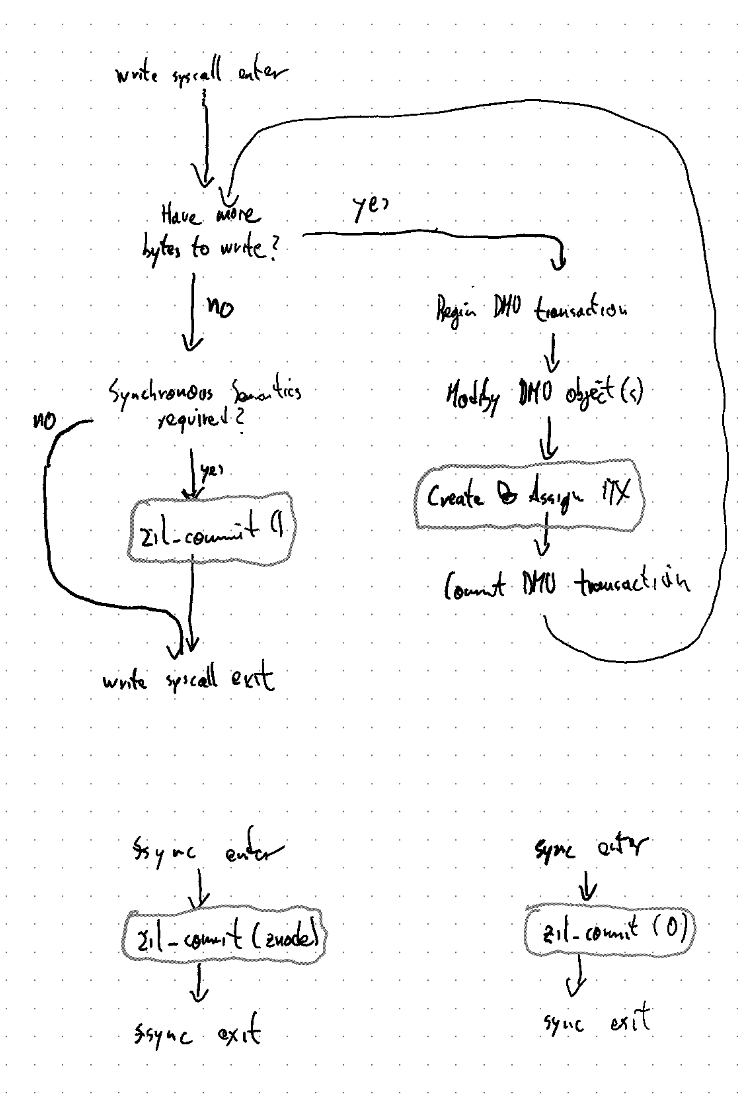
\includegraphics[height=0.8\textheight]{fig/zil_api_syscall_activity_diagram}
    \caption{
        ZIL API usage on the write path in \lstinline{write()}, \lstinline{fsync()}, and \lstinline{sync()} system calls.
    }
    \label{fig:zil_api_syscall_activity_diagrams}
\end{figure}

\lstinline{zilog_t} tracks assigned ITXs in data structures called \lstinline{itxg}.
There exists one \lstinline{itxg} per unsynced pool transaction group (txg).
When an ITX is assigned to the ZIL in a given txg, it is added to that txg's \lstinline{itxg}.
After the txg sync thread has finished syncing a txg, it frees the corresponding \lstinline{itxg} and all the ITXs in it because the changes they describe are now persisted in the main pool and thus obsolete.

Each \lstinline{itxg} is split into a \textit{sync list} and the \textit{async tree}.
The \textit{sync list} is a simple list of ITXs whereas the \textit{async tree} is a search-tree that maps from object ID to a list of ITXs.
By default, ITXs are added to the \textit{sync list} when assigned to the ZIL.
The \textit{async tree} is only used for ITXs that are scoped to a particular file.
For example, an ITX that logs the creation of a file is added to the \textit{sync list} whereas a write within that file is added to the \textit{async tree}.

\lstinline{zil_commit} uses the \lstinline{itxg}s to build a linear \textit{commit list} of ITXs that it can subsequently persist to stable storage.
The pseudo-code in Figure~\ref{lst:zil_commit} illustrates the construction of the commit list by \lstinline{zil_commit}.
Figure~\ref{fig:zil_per_itxg_state_example} provides an example for a single transaction group.
\begin{figure}[h]
    \begin{lstlisting}
zil_commit(object_id)
    commit_list := []
    for each unsynced transaction group 'txg':
        itxg <- the itxg for txg
        if object_id == 0:
            append all itxs in itxg.async to itxg.sync
        else:
            append only the itxs in
              itxg.async[object_Id] to itxg.sync
        append itxg.sync to commit_list
    err := persist commit_list
    if err:
        wait until the open txg has synced
    return
\end{lstlisting}
    \caption{Pseudo-code that illustrates the work done by \lstinline{zil_commit()}.}
    \label{lst:zil_commit}
\end{figure}

\begin{figure}[h]
    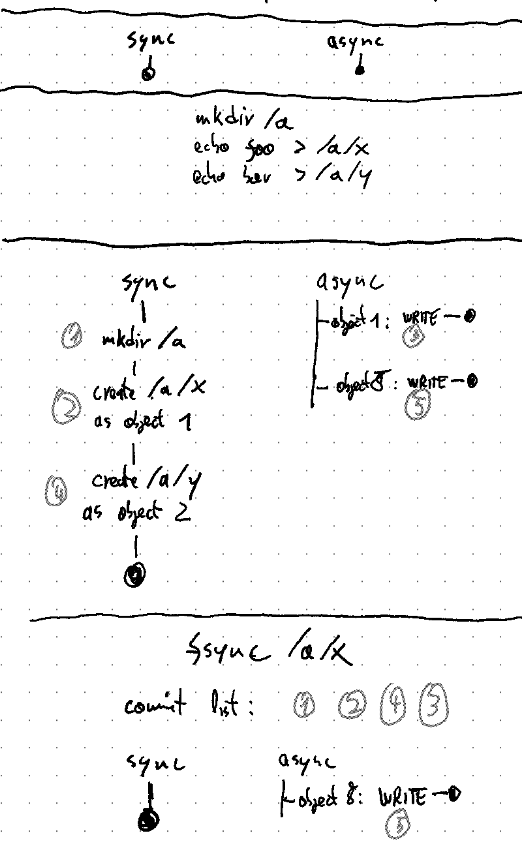
\includegraphics[height=0.5\textheight]{fig/zil_single_itxg_example}
    \caption{
        An example of how an itxg is filled with ITXs and how \lstinline{zil_commit} drains it into a commit list.
        Note that this example only covers the case where all ITXs were assigned for the same txg.
    }
    \label{fig:zil_per_itxg_state_example}
\end{figure}


\chapter{Why ZIL-LWB Is Slow On PMEM}\label{ch:lwb_analysis}
\blindtext\todo{blindtext}

\chapter{Design \& Implementation}
In this chapter we present the design and implementation of ZIL-PMEM in OpenZFS.
We start with an outline of the project goals and limitations, followed by a high-level overview of the design.
Each of the subsequent sections then presents one orthogonal concept in more detail, including implementation aspects where appropriate.
Readers should be familiar with the technical background on PMEM in Linux and OpenZFS given in Section~\todo{ref}.

\section{Project Scope}

\newcommand{\csgoal}[1]{\textbf{#1}}

\subsection{Requirements}\label{sec:requirements}
The following features are success criteria for the ZIL-PMEM design.

\csgoal{Coexistence}
ZIL-PMEM must coexist with ZIL-LWB due to limited availability of PMEM and limitations of the ZIL-PMEM design.

\csgoal{Same Guarantees}
ZIL-PMEM must maintain the same crash consistency guarantees towards user-space as ZIL-LWB for both ZPL and ZVOL.

\csgoal{Simple Administration \& Pooled Storage}
Pooling of storage resources and simple administration are central to ZFS.~\cite{bonwickZettabyteFileSystem2003}
ZFS should automatically detect that a SLOG device is PMEM and, if so, use ZIL-PMEM for all of the pool’s datasets.
No further administrative action should be required to fully benefit from ZIL-PMEM.

\csgoal{Correctness}
In the absence of PMEM media errors and data corruption, ZIL-PMEM must be able to replay all data that it reported as committed.
The result must be the same as if ZIL-LWB would have been used in lieu.
Specifically:
\begin{itemize}[noitemsep,beginpenalty=100000,midpenalty=100000]
    \item Replay must respect the logical dependencies of log entries.
    \item Logging must be crash-consistent, i.e., the in-PMEM state must always be such that replay is correct.
    \item Replay must be crash-consistent, i.e., if the system crashes or loses power replay must be able to resume. Resumed replay must continue to respect logical dependencies of log entries.
\end{itemize}

\csgoal{Data Integrity}
Data integrity is a core feature of ZFS.~\cite{bonwickZettabyteFileSystem2003}
ZIL-PMEM must detect corrupted log entries using an error-detecting code.
Detected corruption must be handled \textit{correctly} as outline in the previous paragraph.
It must also be handled gracefully with the following behavior as the baseline:
"Assume a sequence of log entries $1 \dots N$ where log entry $1$ does not depend on a log entry and each entry $i > 1$ depends on its predecessor $i-1$.
Data corruption in entry $i \in 1 \dots N$ must not prevent replay of entries $1 \dots i-1$".

\csgoal{Low Latency}
The latency overhead of ZIL-PMEM compared to raw PMEM device latency should be minimal for single threaded workloads.
Multi-threaded workloads are addressed below.

\csgoal{Multi-Core Scalability}
Since PMEM is added as a pool-wide resource used by all of the pool's datasets, ZIL-PMEM should scale well to multiple cores.
Barring PMEM throughput limitations, ZIL-PMEM should achieve the following speedups for threads that perform synchronous I/O operations on separate CPU cores:
{
\setlength{\parskip}{0pt}
\begin{description}[topsep=0pt, noitemsep, leftmargin=1cm, labelindent=1cm, widest=1 private dataset per thread]
    \item[1 private dataset per thread] Always near-linear speedup.
    \item[1 shared dataset] \mbox{}
          \begin{description}[noitemsep, leftmargin=1cm, labelindent=1cm, widest=ZPL filesystem]
              \item[ZPL filesystem] No speedup.
              \item[ZVOL] Up to linear speedup, depending on workload.
          \end{description}
\end{description}
}

\csgoal{Maximum Performance On Intel Optane DC Persistent Memory}
Whereas battery-backed NVDIMMs have existed for decades\todo{reference}, Intel Optane DC Persistent Memory is currently the only broadly available flash-based persistent memory product\todo{proof}.
We develop ZIL-PMEM on this platform and want to determine the maximum performance that can be achieved with it.

\csgoal{CPU-Efficient Handling Of PMEM Bandwidth Limits}
The PMEM programming model dictates that I/O wait time is spent on-CPU --- typically at a memory barrier instruction or because the CPU has exhausted its store or load buffer capacity\todo{review terminology; need proof?}.
\citeauthor{yangEmpiricalGuideBehavior2020} have shown that a single Optane DIMM's write bandwidth can be exhausted by one CPU core at \SI{2}{GB/s}.
Write bandwidth decreases to \SI{1}{GB/s} at ten or more CPU cores.
In contrast, DRAM shows a near-linear increase in bandwidth to \SI{60}{GB/s} at 15~threads.~\cite[fig.4]{yangEmpiricalGuideBehavior2020}
In practice, these results imply that on-CPU time is wasted as soon as the system writes to PMEM at higher than maximum device bandwidth.
Since ZIL-PMEM shares PMEM among all datasets in the pool, we expect that such overload situtations will happen in practice.
ZIL-PMEM should thus provide a mechanism to shift excessive PMEM I/O wait time off the CPU.

\csgoal{Testability}
ZIL-PMEM must be architected for testability.
The core algorithms presented in this chapter must be covered by unit tests.
Further, ZIL-PMEM should be integrated into the ztest user-space stress test as well as the SLOG tests of the ZFS Test Suite.

\subsection{Out Of Scope For The Thesis}
The following features were omitted to constrain the scope of the thesis.
We believe that our design can accomodate them without major changes.

\csgoal{Support For OpenZFS Native Encryption}
The ZIL-PMEM design presented in this section does not support OpenZFS native encryption.
Intel Optane DC Persistent Memory supports transparent hardware encryption per DIMM at zero overhead\todo{cite spec}.
In contrast, OpenZFS native encryption is per dataset and software-based.
Given these significant differences in data and threat model, ZIL-PMEM cannot rely on Optane hardware encryption.
Instead, ZIL-PMEM would need to invoke OpenZFS native encryption and decryption routines when writing or replaying log entries.

\csgoal{Protection Against Scribbles}
Scribbles are bugs in the system that accidentally overwrite PMEM, e.g., due to incorrect address calculation or out-of-bounds access in the kernel.
PMEM-specific filesystems such as PMFS and NOVA-Fortis have already introduced mechanisms to protect againt scribbles.~\cite{dulloorSystemSoftwarePersistent2014,xuNOVAFortisFaulttolerantNonvolatile2017}
We believe that our design can be trivially extended with similar mechanisms.

\subsection{Limitations}
The following features were deliberately left out of our design.
More experimentation and experience with ZIL-PMEM will benecessary to determine which features are useful in practice, how they can be realized, and how they interact with the existing requirements.

\csgoal{No NUMA Awareness}
\citeauthor{yangEmpiricalGuideBehavior2020} recommend to "avoid mixed or multi-threaded accesses to remote NUMA nodes. [...]  For writes, remote Optane’s latency is 2.53x (ntstore) and 1.68x higher compared to local"~\cite{yangEmpiricalGuideBehavior2020}.
Given the latency contribution of ZIL-PMEM to overall syscall latency (ref~\ref{ch:eval}\todo{precise ref}), variations of this magnitude would be significant.

\csgoal{No Data Redundancy}
ZIL-PMEM provides data integrity protections but does not provide a mechanism for data redundancy.

\csgoal{Only Works With SLOGs}
ZIL-PMEM only works with PMEM SLOGs, not for a zpool with PMEM as main pool vdevs.
Such pools continue to use ZIL-LWB.

\csgoal{No Software Striping}
Our design only supports a single PMEM SLOG device.
Users may wish to use multiple PMEM DIMMs to increase log write bandwidth.
With Intel Optane DC Persistent Memory, multiple PMEM DIMMs can be interleaved in hardware with near-linear speedup.~\cite{yangEmpiricalGuideBehavior2020}
Whereas software striping would be the natural approach to ZFS, it will be non-trivial to achieve the same speedup as hardware-based interleaving.

\csgoal{No Support For \lstinline{WR_INDIRECT}}
ZIL-LWB logs large write records' data directly to the main pool devices.
The ZIL record then only contains metadata such as \lstinline{mtime} and a block pointer to the location in the main pool.
This technique avoids double-writes which is particularly advantageous if the pool does not have a SLOG which is a case that ZIL-PMEM does not address (see above).
Further, if a SLOG is available, \lstinline{WR_INDIRECT} log record write latency is likely to be dominated by the main pool's IO latency if it consists of regular block devices.
If the main pool's IO latency were acceptable, a fast NVMe-based ZIL-LWB SLOG or no SLOG at all would likely be sufficient for the setup in question.

\csgoal{Space Efficiency}
ZIL-PMEM is allowed to trade PMEM space for time and simplicity when presented with the option.
Our justification is twofold.
First, PMEM capacities are significantly higher than DRAM.
For example, the smallest Intel Optane DC Persistent Memory DIMM offered by Intel is \SI{128}{GiB}.~\cite{optanepricing_missing}
Second, the maximum amount of log entry space required from any ZIL implementation is a function of the maximum amount of dirty data allowed in the zpool.\todo{move to background?}
For ZIL-LWB, small SLOG devices of \SI{16} to \SI{32}{GiB} are sufficient in practice.\todo{ref ix systems truenas M}
Thus, there is sufficient headroom for PMEM space usage in ZIL-PMEM before we need to worry about hardware capacity.


\section{Overview}
This section summarizes the ZIL-PMEM design at a high level.
The subsequent sections then provide more detail on each abstractions' design and implementation.

We introduce the concept of \textit{ZIL kinds} to ZFS.
The ZIL kind is a pool-scoped variable that determines the pool's strategy for persisting ZIL entries.
A zpool's ZIL kind is determined by the following rule:
if the pool has exactly one SLOG and that SLOG is PMEM, the ZIL kind is ZIL-PMEM. Oterwise, it is ZIL-LWB.
ZIL-LWB is the current ZIL's persistence implementation.
It uses the SPA's metaslab allocator to allocate log-write blocks (LWBs) from the storage pool with a bias towards SLOG devices.
ZIL-PMEM disables metaslab allocation for its PMEM SLOG device and uses the PMEM space directy.

The PMEM space is partitioned into fixed-size segments.
Each segment has a corresponding in-DRAM data structure called \textit{chunk} that tracks the segment's kernel-virtual base address and length.
Chunks are organized in a pool-wide in-DRAM data structure called \textit{PRB}.
PRB implements a high-performance, scalable, crash-consistent, data-corruption-checking and garbage-collected write-ahead log.
It stores log entries in the PMEM chunk's segments as a contiguous append-only sequence.
Full chunks are stashed away and become reusable for logging when the youngest entry's transaction group has synced to the main pool.
After a system crash, a new instance of PRB is instantiated with the same chunks (segments) that the pre-crash PRB instance used.
The new instance scans each chunk for log entries that need to be replayed.
This process is called \textit{claiming}.
The entries' physical location in PMEM is irrelevant for replay.
Instead, each entry stores sufficient metadata to determine whether an entry needs to be replayed, to detect missing entries, and to find a deterministic a replay order.
Once claiming is complete, the new PRB instance is ready for replay and logging by datasets.
It only uses those chunks for logging that do not have a replay claim.

PRB is a pool-wide data structure but the ZIL is written and replayed on a per-dataset basis.
For this purpose, PRB defines a data structure called HDL that holds the per-dataset PRB state, such as the log's GUID, dependency-tracking state and replay position.
All interaction that is scoped to a dataset happens through the HDL, not PRB.
Whereas PRB/HDL implements PMEM persistence, it is the HDL user's responsibility to persist HDL state in the main pool.

The keystone to the ZIL-PMEM architecture is the per-dataset in-DRAM struct \lstinline{zilog_t}.
Before the introduction of ZIL kinds, \lstinline{zilog_t} implemented all ZIL-related functionality.
With ZIL kinds, \lstinline{zilog_t} acts as an abstract base class that encapsulates shared ZIL functionality.
This includes the definitions of the ZIL log record format and the data structures that track which log entries need to be persisted when sync semantics are requested by a syscall.
% % for a whole dataset (\lstinline{sync()}), a single file (\lstinline{fsync()}) or an individual syscall (e.g. \lstinline{write()} on an \lstinline{O_SYNC} file descriptors).
The code that is responsible for persisting log entries resides in ZIL-kind-specific subclasses.
The pool's ZIL kind determines which subclass is instantiated at runtime.
The subclass for ZIL-LWB is \lstinline{zilog_lwb_t} which contains the original LWB code.
The subclass for ZIL-PMEM is \lstinline{zilog_pmem_t}.
It is a thin wrapper around HDL's logging and replay methods.
\lstinline{zilog_pmem_t} persists HDL state in the dataset's ZIL header.
The \lstinline{zil_pmem} module --- which defines \lstinline{zilog_pmem_t} --- is the component that integrates PRB/HDL into ZFS:
it allocates the chunks, constructs the PRB and creates and destroys HDLs in synchrony with their datasets.

\begin{figure}[h]
    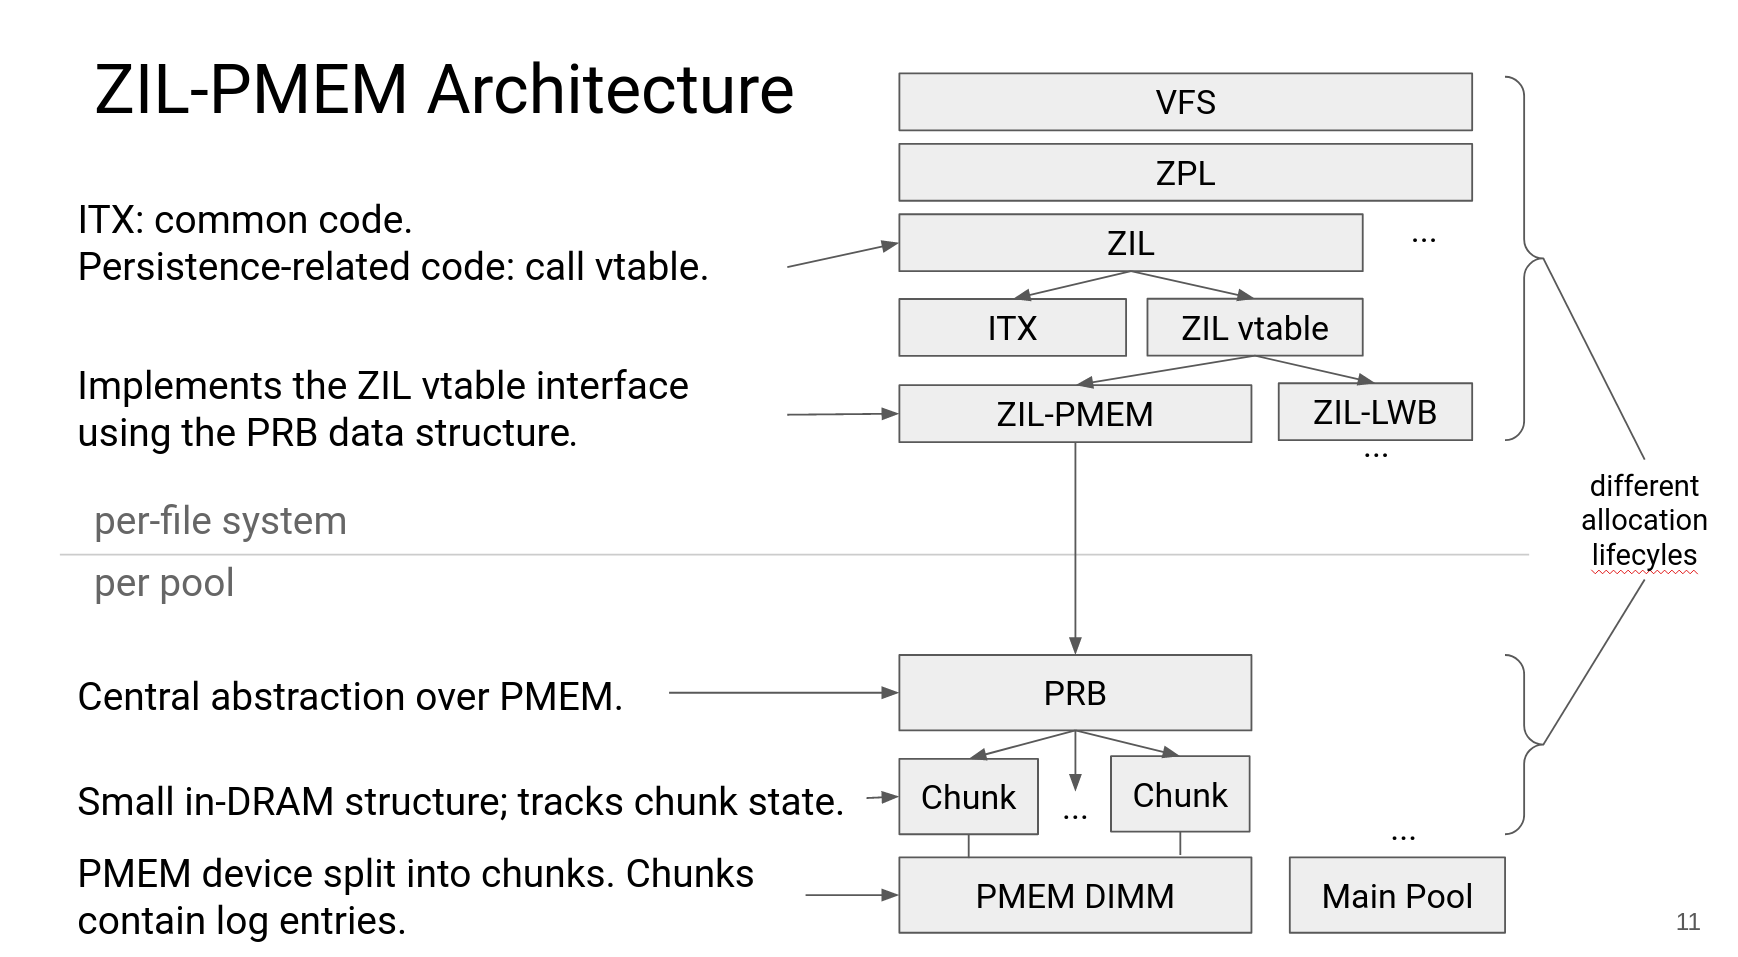
\includegraphics[height=20cm,width=\textwidth,keepaspectratio]{fig/zilpmem_architecture_overview}
    \caption{Overview of the system architecture as described in this section.}
\end{figure}~\todo{actual figure}

\section{ZIL kinds}
Coexistence with the existing ZIL and preservation of ZFS's crash consistency guarantees are two hard requirements for ZIL-PMEM (see Section~\ref{sec:requirements}).
Our solution to both of these problems is to re-architect ZFS to support different persistence strategies for the ZIL while sharing code and data structures that ultimately define crash consistency semantics.
In order to make the integration of ZIL-PMEM seamless to the end user (goal: simple administration), the persistence strategy is the same for all datasets in a pool.
The variable that determines the pool's persistence strategy is its \textit{ZIL kind}.
The following sub-sections present how we refactored ZFS to support ZIL kinds.
The existing ZIL which uses LWBs for persistence becomes the first ZIL kind called ZIL-LWB.
Note that some listings in this section already mention ZIL-PMEM to illustrate why ZIL kinds are necessary to integrate ZIL-PMEM.
However, in our implementation, all refactoring steps presented in this section are separate commits that precede the introduction of the ZIL-PMEM ZIL kind.

\subsection{On-Disk State}\label{sec:di:zil_header}
As described in Section~\ref{openzfs:the_zil_on_disk_format} the ZIL(-LWB) keeps its persistent state in the per-dataset ZIL header and the LWB chain.
For ZIL kinds, we change the ZIL header to be a tagged union that uses the new \lstinline{zh_kind_t} enum as a discriminant.
The existing ZIL-LWB header fields are moved into the \lstinline{zil_header_lwb_t} type.
ZIL-PMEM's ZIL header, which we describe in Section~\ref{sec:zilpmem}, is the second type in that union.
We maintain the same size as the original \lstinline{zil_header_t} by using one 64 bit word of padding, thereby simplifying the on-disk format migration.
Figure~\ref{lst:zil_header_before_and_after} shows the relevant C structures before and after the changes described in this paragraph.

\begin{figure}[h]
\begin{subfigure}[t]{0.45\textwidth}
\begin{lstlisting}
typedef struct zil_header {
  uint64_t zh_claim_txg;
  uint64_t zh_replay_seq;
  blkptr_t zh_log;
  uint64_t zh_claim_blk_seq;
  uint64_t zh_flags;
  uint64_t zh_claim_lr_seq;
  uint64_t zh_pad[3];
} zil_header_t;
\end{lstlisting}
\end{subfigure}
\hfill
\begin{subfigure}[t]{0.5\textwidth}
\begin{lstlisting}
typedef enum {
    ZIL_KIND_UNINIT,
    ZIL_KIND_LWB,
    ZIL_KIND_PMEM,
    ZIL_KIND_COUNT
} zh_kind_t;

typedef
struct zil_header_lwb {
  /* fields of zil_header_t,
   * without zh_pad */
} zil_header_pmem_t;

typedef
struct zil_header_pmem {
  /* introduced later */
} zil_header_pmem_t;

typedef
struct zil_header {
  uint64_t zh_kind;
  union {
    zil_header_lwb_t  zh_lwb;
    zil_header_pmem_t zh_pmem;
  } zh_data;
  uint64_t zh_pad[2];
} zil_header_t;
\end{lstlisting}
\end{subfigure}
\caption{The ZIL header structs (in DRAM and on disk) before and after the introduction of ZIL kinds.}
\label{lst:zil_header_before_and_after}
\end{figure}

\subsection{Runtime State}\label{sec:zil_kinds:runtime}
As described in Section~\ref{openzfs:the_zil_api}, the ZIL(-LWB) runtime state is kept in the per-dataset object \lstinline{zilog_t}.
\lstinline{zilog_t} tracks the in-memory representation of log records (ITXs) in the \lstinline{itxg} struct until they become obsolete due to txg sync or need to be written to stable storage by \lstinline{zil_commit}.
\lstinline{zil_commit} drains the ITXs into the \textit{commit list}.
It proceeds by packing the ITXs on the commit list into LWBs which it writes to disk as a chain linked by ZFS block pointers.

We observe the following properties of the code that handles ITXs and \lstinline{itxgs}:
\begin{itemize}[noitemsep]
    \item It defines the framework for ZFS's crash consistency semantics.
          Whereas ZPL and ZVOL code fill the body of the log records, the organization by \lstinline{itxgs} and the code that assembles the commit list constraints what can be expressed as ZIL records.
    \item ITXs and even the commit list are independent of the LWB chain that is ultimately written to disk.
          The commit list merely defines the set of ZIL records that need to be persisted before \lstinline{zil_commit} can return, and in what order these log records must be replayed.
    \item The interface between the ITX- and LWB-related code is limited to the \textit{commit list} and its contents.
          Whereas the ITXs are not opaque to the LWB-related code (e.g. handling of \lstinline{WR_NEED_COPY}\todo{check that this was defined}), the responsibilities are cleanly separated.
\end{itemize}
Given these insights we refactor the ZIL implementation (\textit{zil.c}) as follows:
\begin{enumerate}[noitemsep]
    \item Move all non-ITX functions into a separate module \textit{zil\_lwb.c} and prefix them with \lstinline{zillwb_}.
          If the function was part of the public ZIL API, add a wrapper function with the original name to \textit{zil.c} that forwards the call to the \lstinline{zillwb_} function in \textit{zil\_lwb.c}.
    \item Virtualize calls to \lstinline{zillwb_} functions in \textit{zil.c}:
          \begin{itemize}
              \item Define a struct \lstinline{zil_vtable_t} that contains function pointers with the type signature of each of the \lstinline{zillwb_} functions called from \textit{zil.c}.
              \item Define \lstinline{zillwb_vtable} as an instance of \lstinline{zil_vtable_t} that uses \lstinline{zillwb_} functions as values for the respective function pointer members.
              \item Add a member \lstinline{zl_vtable} to \lstinline{zilog_t} that is pointer to a \lstinline{zil_vtable_t}.
              \item Replace all calls to \lstinline{zillwb_FN()} in \textit{zil.c} with indirect calls through the vtable, i.e., \lstinline{zilog->zl_vtable.FN()}.
          \end{itemize}
    \item Make non-ITX state private to \textit{zil\_lwb.c} by turning it into a subobject.
          \begin{itemize}
              \item Move the \lstinline{zilog_t} members that are only used by the functions in \textit{zil\_lwb.c} into a separate structure called \lstinline{zilog_lwb_t} that is private to \textit{zil\_lwb.c}.
              \item Embed \lstinline{zilog_t} as the first member in \lstinline{zilog_lwb_t}.
              \item Add member \lstinline{zlvt_alloc_size} to \lstinline{zl_vtable_t} that indicates the amount of memory to be allocated when allocating a \lstinline{zilog_t}.
              \item Add a \textit{downcast} step to the start of each \lstinline{zillwb_} function that casts the \lstinline{zilog_t} pointer into a \lstinline{zilog_lwb_t} pointer.
                The majority of functions can operate only on the \lstinline{zilog_lwb_t}-private state without accessing the embedded \lstinline{zilog_t}.
              \item Add constructor and destructor methods to the vtable that are called after allocating the \lstinline{zlvt_alloc_size}d \lstinline{zilog_t}.
                The \lstinline{zillwb_} constructor and destructors initialize and deinitialize the private members of \lstinline{zilog_lwb_t}.
          \end{itemize}
\end{enumerate}
The end result ist best described in the terminology of object-oriented programming:
\textbf{\lstinline{zilog_t} is an abstract baseclass} that implements the public ZIL interface as well as ITX-related functionality and defines abstract methods for persisting log records.
These abstract methods must be implemented by concrete subclasses.
\lstinline{zilog_lwb_t} is such a subclass that implements the LWB-based persistence strategy.
For ZIL-PMEM, the \lstinline{zilog_pmem_t} struct which we introduce in Section~\ref{sec:zilpmem} implements persistence directly to PMEM.
Which subclass is instantiated at runtime is determined by the \lstinline{zh_kind} field in the ZIL header (see Section~\ref{sec:di:zil_header} and Figure~\ref{lst:zil_header_before_and_after}).
Figures~\ref{fig:zilog_splitup_class_diagram} and \ref{fig:zilog_splitup_example_code} illustrate the changes described in this section.

\begin{figure}
\missingfigure[figheight=10cm]{}
\caption{\lstinline{zilog_t} before and after the introduction of ZIL kinds, visualized as a class diagram.}
\label{fig:zilog_splitup_class_diagram}
\end{figure}

\begin{figure}
\missingfigure[figheight=20cm]{}
\caption{The refactoring steps described in Section~\ref{sec:zil_kinds:runtime} by example of the \lstinline{zil_itx_assign()} and \lstinline{zil_commit()} APIs.}
\label{fig:zilog_splitup_example_code}
\end{figure}

\subsection{Changing ZIL Kinds}\label{sec:zil_kinds:change}
In the design overview (sec.~\ref{sec:design_overview}) we introduce ZIL kinds as a pool-scoped variable.
The pool's ZIL kind implicitly according to the following rule:
\begin{displayquote}
If the pool has exactly one SLOG and that SLOG is PMEM, the ZIL kind is ZIL-PMEM. Oterwise, it is ZIL-LWB.
\end{displayquote}
The rule is re-evaluated whenever a SLOG is added or removed, i.e., during pool creation and on \texttt{zpool add} and \texttt{zpool remove}.
The idea behind this approach is to keep administration simple --- a defining paradigm for ZFS:
ZIL-PMEM should be automatically activated if hardware and software support it and not be used otherwise.
%Note that the alternative significantly worsens\todo{that a word?} the user experience since they would need to configure the ZIL kind of each individual dataset, or rely on some auto-tuning mechanism.

To accomplish this behavior, the following steps must happen in the same transaction group as the SLOG addition or removal that triggered the change of ZIL kind:
\begin{enumerate}[noitemsep]
    \item Stop using the ZIL API and wait until all active calls to it have finished.
    \item Wait for all ZIL entries to become obsolete by waiting for the open txg to sync.
    \item \lstinline{zil_close()} and subsequently \lstinline{free()} the currently open \lstinline{zilog_t} instances.
    \item Replace all datasets' ZIL header with the new ZIL kind's default header.
        \lstinline{zh_kind} is now set to the new ZIL kind.
    \item Allocate the new \lstinline{zilog_t} instances and \lstinline{zil_open()} them.
        The allocation routine uses \lstinline{zh_kind} to select the (new) vtable, allocates \lstinline{zlvt_alloc_size} bytes for the new \lstinline{zilog_KIND_t} and runs the ZIL kind specific constructor.
\end{enumerate}
Due to time constraints we have \textbf{not yet implemented} this procedure.
As a stop-gap solution, we add a kernel module parameter \lstinline{zil_default_kind} that defines the ZIL kind that is used for the \lstinline{zh_kind} field in new dataset's ZIL headers.
There is no mechanism to change \lstinline{zh_kind} over the lifetime of a dataset.
It is possible to mix different ZIL kinds in the same pool by changing \lstinline{zil_default_kind} before creating a new dataset.
This works correctly but is undesirable from a usability perspective because we want ZIL kinds to be transparent to the user.
% DON'T point out that the design alternative is to have internal polymorphism within zilog_t. It's trivial to see from an implementor's perspective.

\subsection{ZIL-LWB Suspend \& Resume}\label{sec:zil_kinds:suspend_resume}
The ZIL API provides the \lstinline{zil_suspend} and \lstinline{zil_resume} functions.
\lstinline{zil_suspend} pauses all ZIL activity and ensures that all log entries are obsolete.
\lstinline{zil_resume} reverts the state to normal operation.
Compatibility code for versions of ZFS prior to the \textit{fast snapshots} feature must use them for snapshots.
For newer pool versions, the only consumer \lstinline{spa_reset_logs}: when removing a SLOG from the pool, the ZIL is temporarily suspended to ensure that the SLOG does not contain valid log entries.
Once the ZIL resumes and starts allocating LWBs, the metaslab allocator transparently uses other SLOGs or the main pool devices.

With regards to ZIL kinds, only the \lstinline{spa_reset_logs} use case is relevant since ZIL kinds require a more recent pool version than the \textit{fast snapshots} feature.
Our design for changing ZIL kinds (Section~\ref{sec:zil_kinds:change}) requires suspension of all ZIL activity and thus subsumes the ZIL-LWB specific \lstinline{zil_suspend} and \lstinline{zil_resume}.
However, the compatibility code for pools before \textit{fast snapshots} needs to be maintained in a way that does not depend on the ZIL kinds feature.
Due to time constraints, we were \textbf{unable to address suspend \& resume in our design}.
We expect that the solution will be highly dependent on implementation-level constraints.

\subsection{ZIL Traversal \& ZDB}\label{sec:zil_kinds:traversal}
Whereas ZIL replay is abstracted away by the \lstinline{zilog_t} refactoring, there are several cases where the raw ZIL-LWB chain is traversed directly using the \lstinline{zil_parse} function.
\lstinline{zil_parse} exposes several ZIL-LWB implementation details to its callers such as the concept of LWBs and blockpointers.
This is problematic for ZIL kinds because not every conceivable ZIL kind uses these concepts; ZIL-PMEM being the obvious example.
We investigate all users of the ZIL traversal code and come to the conclusion that there is no need for a generalized interface that every ZIL kind needs to implement.
The basis for this decision is a manual analysis of \lstinline{zil_parse}'s callers.
\begin{description}[noitemsep]
    \item[dmu\_traverse] This module implements a callback-based traversal of the zpool's data structures.
    It is used to implement many ZFS features, e.g., \textit{zfs send}.
    If a dataset is traversed that is a head dataset (i.e., not a snapshot) and its LWB chain has been claimed, the LWBs are included in the traversal.
    \item[dsl\_scan\_zil] During a \textit{zpool scrub} (data integrity check of the entire pool), this function traverses claimed LWB chains.
    \item[spa\_load\_verify] During pool import this function uses \textit{dmu\_traverse} to traverse data structures updated in the last synced transaction groups.
    \item[zdb\_il.c] The \textit{ZFS debugger} interprets the ZIL header of head datasets, traverses their LWB chain, and dumps its contents to stdout.
\end{description}
Most consumers of \textit{dmu\_traverse} operate on snapshots, not head datasets, and therefore do not trigger ZIL chain traversal.
The \textit{dsl\_scan} and \textit{spa\_load} code does not actually use the ZIL data because the data integrity checks are implemented transparently in the ZIO read pipeline.
One compatibility code path (\lstinline{old_synchronous_dataset_destroy}) uses ZIL traversal to free the ZIL blocks, but can be replaced with a more recent API (\lstinline{zil_destroy_sync}).
\textit{zdb} is an exception since its whole purpose is to interpret the ZIL chain for debugging purposes.

Given this analysis we implement the following change as a precursor to the refactoring of \lstinline{zilog_t} described in Section~\ref{sec:zil_kinds:runtime}.
We change the \lstinline{zil_parse} API to work directly on a \lstinline{zil_header_lwb_t*} instead of \lstinline{zilog_t}.
We also rename the function to \lstinline{zillwb_parse_phys} to reflect the fact that it is specific to ZIL-LWB and does not affect runtime state.
Finally, we change the \textit{dmu\_traverse} API so that callers must be explicit about ZIL-LWB traversal which we believe will ease maintainability in the future.
We \lstinline{zil_destroy_sync} in \lstinline{old_synchronous_dataset_destroy}, leaving \lstinline{spa_load_verify} as the only consumer of the \textit{dmu\_traverse} API that needs to traverse ZIL-LWB chain.


\subsection{ZIL-LWB-Specific Callbacks}\label{sec:zil_kinds:callbacks}
There are several callbacks from modules outside of ZIL-LWB.
Since these callbacks are made through static function calls --- not function pointers --- they are part of the ZIL's public API and need to be considered for our ZIL kind refactoring.
However, none of them are necessary for ZIL-PMEM.
Therefore, we prefix the callback functions with \lstinline{zillwb_}, move them to \textit{zil\_lwb.c} and ignore them in the remainder of this thesis.
For maintainability, future work should replace these statically dispatched callbacks with dynamic callbacks through function pointers to increase decoupling.
We list the APIs in question so that this issue can be addressed in future work:
\begin{description}
    \item[zil\_lwb\_add\_txg] Necessary to keep the in-DRAM representation of an LWB alive when writing \lstinline{WR_INDIRECT} blocks.
    \textbf{Note}: we can only afford to ignore this function because ZIL-PMEM does not support \lstinline{WR_INDIRECT} blocks.
    \item[zil\_lwb\_add\_block] Necessary for an optimization that minimizes the amount of flush commands that are sent to the SLOG device.
    \item[zil\_bp\_tree\_add] During a ZIL traversal with \lstinline{zil_parse}, this API was used to avoid doing operation more than once for a given blockpointer.
        It is an implementation detail of ZIL-LWB that is only a public ZIL API because it is used by \textit{zdb}'s ZIL traversal code.
\end{description}

\subsection{Considered Alternatives}
The general concept of ZIL kinds and the vtable-based implementation add complexity to the ZIL code.
In this section we discuss the alternatives that we considered for supporting multilpe ZIL implementations at runtime.

\textbf{Alternative \#1}: We considered moving the dispatch into ZIL kind specific code one API layer up so that \lstinline{zilog_t} and ITX would be completely specific to ZIL-LWB.
The API layer that we considered are the \lstinline{zfs_log_OP} and \lstinline{zvol_log_OP} helper functions which create and assign ITXs for ZPL and ZVOL operations.
The sequence diagram in Figure~\ref{fig:zfs_log_write_sequence_diagram} provides an example of how a \lstinline{write} system call uses this API.
Declaring this API layer the interface for ZIL kinds would allow ZIL implementations to chose freely how they want to represent log records in DRAM and on stable storage.
This additional freedom could be used by future ZIL kinds to implement a different log structure with better scalability or more fine-grained crash consistency guarantees.
For example, an earlier design for ZIL-PMEM used a graph-based log structure where log entries for a file in the same dataset could be written in parallel.
However, the additional freedom also has significant drawbacks that ultimately led us to the design presented in the previous subsections:
\begin{enumerate}[noitemsep]
    \item The \lstinline{zfs_log_OP} family of functions only addresses the ZIL write path.
        There are no equivalent abstractions that wrap the \lstinline{zilog_t} APIs for ZIL replay or traversal.
        In order to have a single clean abstraction at the level of \lstinline{zfs_log_OP}, it would be necessary to extend this API so that \lstinline{zilog_t} could be hidden as an implementation detail of ZIL-LWB.
        We were not confident in our ability to design this API extension without the risk of introducing a leaky abstraction.
    \item ZIL kind specific functions for logging would also require ZIL kind specific replay functions.
        In ZIL-LWB this is a non-trivial amount of code.
        ZIL kinds such as ZIL-LWB that only implement a different persistence strategy would have to duplicate this code, pointlessly increasing maintenance cost.
    \item We find it undesirable to allow ZIL-kinds to implement different crash consistency guarantees, in particular if ZIL kinds switch automatically depending on SLOG hardware (see Section~\ref{sec:zil_kinds:change}).
        Centralizing the ITX code and forcing every ZIL kind to fit into the ITX model is the best way to ensure that crash consistency guarantees are the same across ZIL kinds.
\end{enumerate}

\begin{figure}
    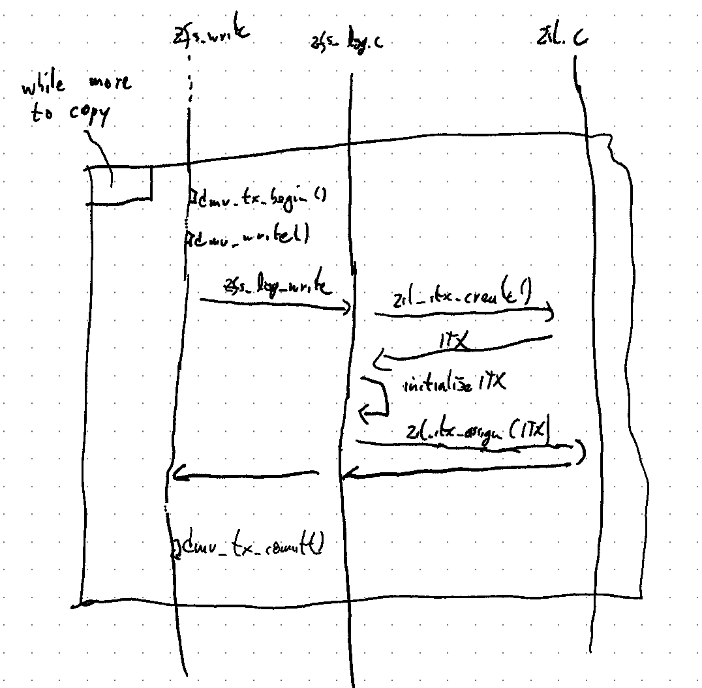
\includegraphics[height=8cm]{fig/zfs_log_write_sequence_diagram}
    \label{fig:zfs_log_write_sequence_diagram}
    \caption{Sequence diagram of the APIs involved in creating the ITXs for a \lstinline{write} system call.}
\end{figure}

\textbf{Alternative \#2}: Since we identified the ZIO pipeline as the main source of latency\todo{ref chapter} in ZIL-LWB, we considered sharing LWBs as a concept between all ZIL kinds.
In that scenario, the ZIL kinds would merely be an alternative to the ZIO pipeline.
A prototype that adopts this approach has been presented at the OpenZFS 2020 Developer summit by \citeauthor{openzfsZILPerformanceImprovements2020}, targeting NVMe drives \cite{openzfsZILPerformanceImprovements2020}
We found this layer of the ZFS software stack to be too restrictive for ZIL-PMEM:
\begin{enumerate}
    \item The timeout mechanism\todo{ref} for packing multiple entries into a single LWB would add unnecessary latency overhead.
        This is in conflict with one of our requirements (see Section~\ref{sec:requirements}).
    \item This notion is shared by the database community which has deemed group commit schemes --- such as LWB timeout --- unfit for PMEM (see Section~\ref{relw:groupcommit}).
    \item The PRB's feature to log entries for the same dataset in parallel\todo{ref} would not have been possible if ZIL-PMEM would be constrained to LWBs.
        Our ITXG bypass for ZVOLs (see Section~\ref{sec:itxg_bypass}) shows how we can use this PRB feature to increase scalability\todo{check,ref} without compromising on crash consistency guarantees.
\end{enumerate}

\subsection{Summary}
We believe that our design for ZIL kinds introduces ZIL kind specific behavior at the layer that allows for sufficient flexibility in the implementation without adding unnecessary abstractions and maintenance burden.
The interface defined by the vtable is a clean abstraction although some design questions (see \ref{sec:zil_kinds:change} and \ref{sec:zil_kinds:suspend_resume}) as well as some LWB-specific APIs (see \ref{sec:zil_kinds:traversal} and \ref{sec:zil_kinds:callbacks}) remain.
The state of each \lstinline{zilog_KIND_t} is truly private do the ZIL kind's implementation.
Neither ZIL-LWB nor ZIL-PMEM access the ITX-related state in the embedded \lstinline{zilog_t} directly, but only\todo{"sondern"?} through the \lstinline{zilog_t} method that computes the commit list.
If requirements change in the future, the design alternatives presented in the previous section should be considered.

\section{PMEM-aware SPA \& VDEV layer}
In this section we describe how we add explicit support for PMEM to ZFS.
Our primary goal is to disable the SPA's metaslab allocation on PMEM SLOG devices so that ZIL-PMEM can use the allocatable space as PRB chunks.

We add a new boolean attribute \lstinline{is_dax} for \lstinline{disk} VDEVs in the zpool config format.
The attribute indicates whether the VDEV supports direct access through the DAX APIs.
Its value is determined by the \lstinline{zpool} command when creating or adding devices to a pool using \lstinline{libblkid}.
When opening a vdev marked \lstinline{is_dax}, the kernel module ensures that all of the block device's sectors are mappable as one contiguous range of kernel virtual address space.
Failure to establish this mapping fails the onlining process, leaving the vdev in state \lstinline{VDEV_STATE_CANT_OPEN}.
By default, this state prevents the pool from being imported.
If the VDEV is added as a log device, the import process allows the user to specify an override flag, causing the log to be dropped.
Note that the \lstinline{is_dax} feature applies to all VDEVs and is independent of ZIL-PMEM.
It merely records the fact that a VDEV is required to be directly accissble via the DAX APIs.

To disable metaslab allocation on PMEM SLOGs, we introduce a new allocation class called \lstinline{exempt}.
When adding a log device to the pool that is \lstinline{is_dax}, the \lstinline{zpool} command assigns it to the \lstinline{exempt} class instead of the \lstinline{log} class.
This alone is sufficient to prevent allocation from PMEM SLOGs because the \lstinline{exempt} allocation class by convention is never used.
The allocatable space on the device is thus never read or written through ZIO and available for use by ZIL-PMEM.
Note that reads and writes to VDEV labels\todo{need to explain this? short analogy: partition header} are located outside of the allocatable space.
Updates to VDEV labels continue to be made using block device IO (\lstinline{zio_read_phys} and \lstinline{zio_write_phys}).

\begin{figure}[h]
    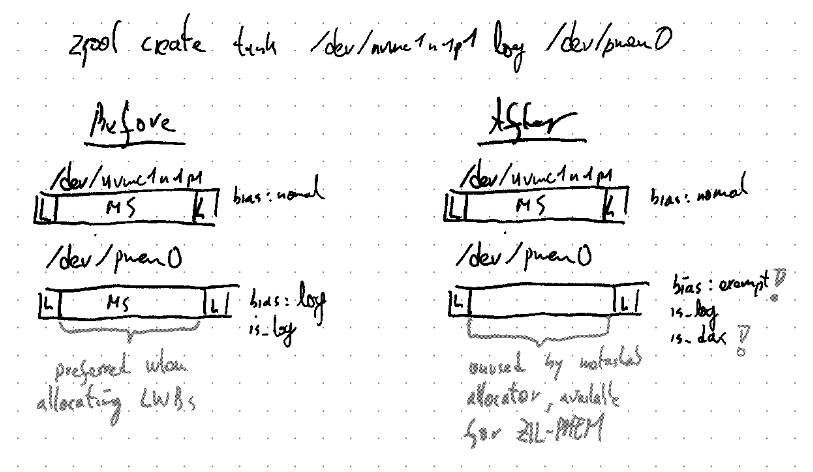
\includegraphics[width=\textwidth]{fig/pmem_aware_vdev_layer_before_after}
    \caption{
        Comparison of the zpool layout before and after the addition of the \lstinline{is_dax} vdev attribute and the \lstinline{exempt} allocation class for PMEM SLOGs.
    }
\end{figure}

\clearpage
\section{PRB/HDL}
In this section we describe the PRB data structure which implements the bulk of ZIL-PMEM's functionality.
PRB abstracts shared physical PMEM into virtual logs for each dataset in the pool.
The \textit{zil\_pmem.c} module (Section~\ref{sec:zilpmem}\todo{chapter}) uses these virtual logs to implement the ZIL-PMEM ZIL kind.
%A single PRB instance supports multiple logs with independent lifecycles.
%Each log is represented by a HDL object that provides methods for writing and replaying log entries.
%Log entries are opaque to PRB --- the only ZFS-specific metadata is the transaction group (txg) in which the log entry's effect will be synced.
%Knowledge of the entry's txg is necessary for log replay and log entry garbage collection.
%The \textit{zil\_pmem.c} module, which we present in Section~\ref{sec:zilpmem}, acts as a mere integration layer between the remainder of ZFS and PRB.
We present the design and implementation of PRB in a top-down manner.
In Section~\ref{di:prb:background} we recapitulate the role of the ZIL in ZFS to isolate ZIL-PMEM's requirements toward PRB.
Afterwards, in Section~\ref{di:prb:structure}, we present the mental modal for the log abstraction exposed by PRB.
We proceed with a description of the API that PRB exposes toward \textit{zil\_pmem.c} (Section~\ref{di:prb:api}).
Equipped with a black-box understanding of PRB's functionality we proceed with the internal design and implementation.
In Section~\ref{di:prb:persistent} we describe PRB's persistent data structure.
The design and implementation techniques of the scalability-oriented write path are presented in Section~\ref{di:prb:write}.
Finally, Section~\ref{di:prb:recovery} describes\todo{word} the algorithms used on the recovery path.

\subsection{Background}\label{di:prb:background}
Remember from section \ref{openzfs:pool_operation} that whenever a file system call changes a dataset $D$, it does so in a DMU transaction $T_i$ within a transaction group $T_{i_{txg}}$.
After the system call handler has finished the DMU transaction by calling \lstinline{dmu_tx_commit(T_i)}, the logical change $C_i$ made in $T_i$ is not yet persisted to stable storage.
Instead, the DMU accumulates the changes from many DMU transactions in DRAM as so-called \textit{dirty state}, grouped by the transaction's txg.
Eventually, the \textit{txg sync} background thread syncs out a new version of the zpool state that contains the accumulated changes of the txg:
it first \textit{quiesces} the currently \textit{open txg} by not admitting new DMU transactions to it and waits for existing DMU transactions to finish.
Once all DMU transactions have finished, it is guaranteeed that the accumulated dirty state for this txg is not going not change.
The txg transitions to the \textit{syncing} state and txg sync starts to write out an updated version of the on-disk state.
After this process is complete, the transaction group is the pool's new \textit{last synced} txg.
Note that there are three unsynced txgs at any given time, one for each of the three states \textit{open}, \textit{quiescing}, and \textit{syncing}.
This improves DMU transaction latency because it decouples new DMU transactions from the \textit{txg sync} thread:
new DMU transactions can always operate on the open txg while txg sync only operates on the syncing txg.

The purpose of the ZIL is to bridge the gap between the time at which a DMU transaction $T_i$ is finished (\lstinline{dmu_tx_commit}) and the time at which the changes made by $T_i$ actually reach the main pool through \textit{txg sync}.
For that purpose, the system call handler encodes the change $C_i$ that was made in $T_i$ as a \textit{log record}, wraps it in an \textit{ITX} and \textit{assigns} it to the ZIL.
If the system call has synchronous semantics, the system call handler invokes \lstinline{zil_commit} before returning to userspace.
\lstinline{zil_commit} uses the \lstinline{itxg} data structure to determine the sequence of log records that needs to be written out to persistent storage.
This sequence is called the \textit{commit list}.
At this point, the ZIL-kind specific implementation takes over: it is responsible for concatenating the current \lstinline{zil_commit} call's commit list to previously written commit lists.
The logical structure of the log, regardless of ZIL kind, is thus a sequential chain of log records that is extended by \lstinline{zil_commit}.

After a system crash, the zpool is in the state of the last synced transaction group which we call \textit{precrash-txg}.
Our dataset $D$ is lacking exactly those changes $C_i$ whose transactions $T_i$ were made in transaction groups younger than precrash-txg (their $T_{i_{txg}} > precrash\text{-}txg$).
When $D$ is mounted, these changes $C_i$ need to be applied to $D$ in order to recover data that was reported as committed towards userspace.
The ZIL API for this task is called \lstinline{zil_replay}.
Its implementation is specific to each ZIL kind but the API contract is the same:
the caller provides a callback that the implementation invokes for every log record that represents a missing change $C_i$.
The callback interprets the log record and performs a DMU transaction that atomically applies the change to the dataset and records replay progress in the ZIL header.
The invocation order is given by the commit list, but entries for transactions before or in precrash-txg ($T_{i_{txg}} \le precrash\text{-}txg$) must be skipped because the change encoded in them is already part of the dataset state.
We provide an example for the commit list and the replay sequence for different precrash-txgs in Figure~\ref{fig:zil_writepath_and_replay_sequence_logical_level}.

\begin{figure}[H]
    \centering
    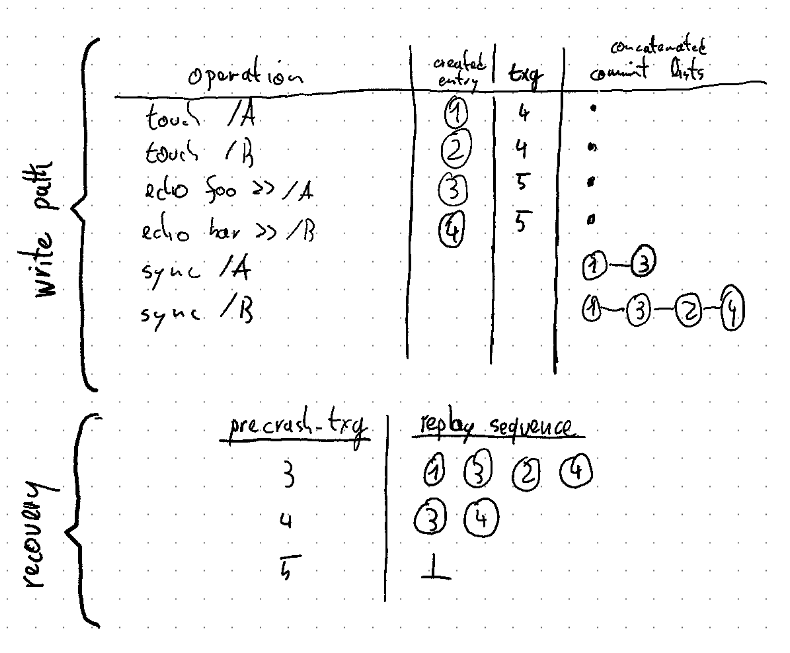
\includegraphics[height=7cm]{fig/zil_writepath_and_replay_sequence_logical_level}
    \caption{
        Example for a commit list with entries from different files and txgs.
        We show the replay sequences for different precrash-txgs.
        The replay callback must only be invoked for the entries that log changes in txgs younger than the precrash-txg.
    }
    \label{fig:zil_writepath_and_replay_sequence_logical_level}
\end{figure}


\subsection{Model}\label{di:prb:structure}
We identify the following requirements for the persistence layer of any ZIL kind:
\begin{itemize}[noitemsep]
\item On the write path, it needs to append entries to a log that is synchronously persisted to stable storage.
\item In the event of a crash, it needs to recover the exact subset of log records that represent changes that have not been synced to the main pool.
    It must be able to sort the subset by insertion order.
\item Finally, since storage is pooled in ZFS, there needs to be an abstraction that constructs such a log from the pool's raw storage space.
    \todo{LWBs + metaslab + ZIO for ZIL-PMEM, is that clear or should we explain? see how the next paragraph starts.}
% the ZIL is a per-dataset log but we add PMEM as a shared resource to the pool, ZIL-PMEM needs an abstraction that virtualizes the physical PMEM space into per-dataset logs.
\end{itemize}

PRB is our solution to address these requirements in ZIL-PMEM.
The PRB is an in-DRAM structure that exists once per zpool.
A pool's PRB instance is allocated during pool import and set up with many segments of PMEM (\textit{chunks}).
For each dataset in the zpool, PRB exposes a \textit{HDL} which implements a virtual log that is persisted in the PMEM chunks.
The log is created when dataset is first mounted and is subsequently used for writing log entries.
Log entries can only be appended and are automatically garbage-collected after their transaction group has been synced out by txg sync.
HDLs are never read except during recovery after a system crash.
For that purpose, HDL implements the callback-based replay interface described in the previous section:
the HDL consumer provides a callback that is invoked for exactly those entries whose changes were made in transactions younger than the precrash-txg.

The unit that can be written to a log is the \textit{log entry}.
It is the representation of a logical change $C_i$ that was made in a DMU transaction $T_i$ within a transaction group $T_{i_{txg}}$.
The log entry's payload is an opaque binary blob that encodes the change $C_i$.
It is the log writer's and replay callback's responsibility to define the encoding.
PRB then guarantees data integrity using checksums and handles machine check exceptions raised by the PMEM hardware.

HDL allows for limited parallelism when writing log entries.
The motivation for this feature is that the sequentiality inherent in the \textit{commit list} model is a scalability bottleneck.
For example, if multiple threads modify the same file simultaneously, their modifications cannot be causally dependent and could be logged in parallel without coordination.
If the storage medium can maintain low latency for these parallel writes, overall throughput can be improved without latency cost.
But since the ZIL's logical structure is that of a concatenation of commit list, the log writers are bound to serialize their writes to the log.
We present an application of parallel logging for ZVOLs in Section~\ref{sec:itxgbypass}.
Our evaluation in Section~\ref{ch:eval}\todo{precise} demonstrates that significant scalability improvements over ZIL-PMEM with sequential commit lists are possible without weakening crash consistency guarantees.

The logical structure of the log is complicated by the support for parallel writers.
To describe it, we introduce the concept of \textit{generations}:
the HDL log is structured as a sequence of generations, each of which contains many log entries.
The most recent generation in the log is called the \textit{open generation}.
When a thread writes a log entry, it must indicate whether the entry should be written to the open generation or whether a new generation should be started.
If no new generation is started, the log entry is allowed to be written in parallel with other threads that also write to the open generation.

Generation assignment is critical for replay correctness because generation membership encodes logical dependencies between entries.
The dependency relationship induced by generations is defines as follows:
\begin{displayquote}
Entries within the same generation do not depend on each other.
Entries from newer generations unconditionally depend on all entries in all previous generations.
\end{displayquote}
Thus, if an entry $E$ depends on an entry $E'$ that is missing and $E'$'s txg is younger (i.e., greater than) than the precrash-txg, replay stops with an error at entry $E$.
Figure~\ref{fig:prb_logical_structure} provides three examples for the log structures that can be expressed using \textit{generations}, and how generation assignment affects log recovery.

\begin{figure}[H]
    \begin{subfigure}{\textwidth}
        \centering
        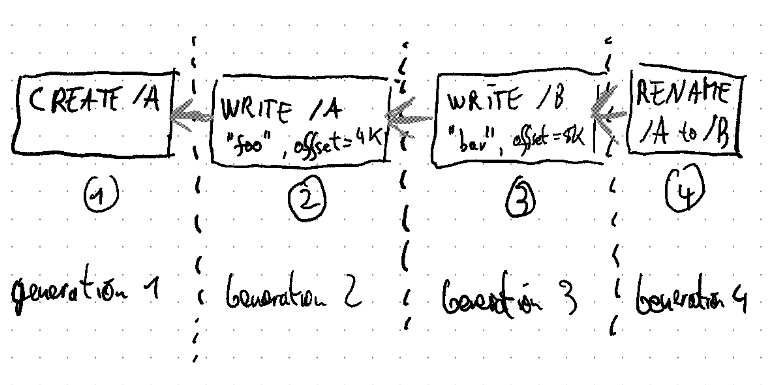
\includegraphics[height=4cm]{fig/prb_logical_structure__seqchain}
        \caption{
            Each entry was written to a new generation, resulting in a sequence of dependent entries.
            This structure corresponds to the model of concatenated commit lists defined by the ITX layer.
            However, only entries 3 and 5 must be replayed.
            If entries 1, 2, and 4 were missing, replay would still succeed.
        }
        \label{fig:prb_logical_structure:seqchain}
    \end{subfigure}
    \begin{subfigure}{\textwidth}
        \centering
        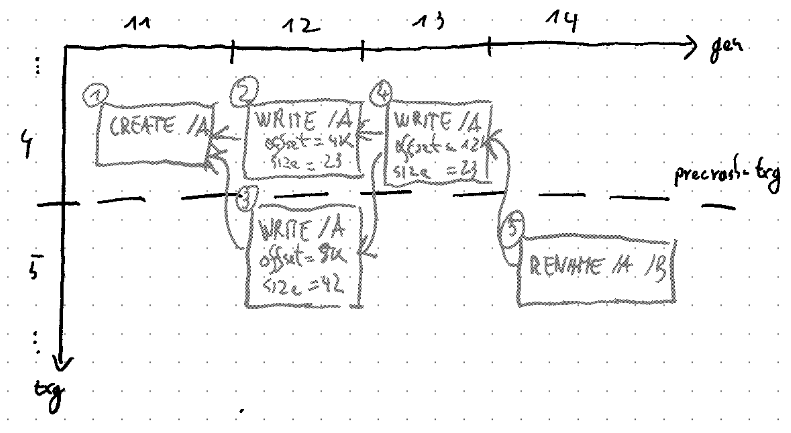
\includegraphics[height=4cm]{fig/prb_logical_structure__diamondchain}
        \caption{
            Entries 2 and 3 were written in the same generation, possibly in parallel.
            Entry 4 was written in the next generation and thus logically depends on both entries 2 and 3.
            However, only entries 3 and 5 must be replayed.
            If entries 1, 2, and 4 were missing, replay would still succeed.
            }
        \label{fig:prb_logical_structure:diamondchain}
    \end{subfigure}
    \begin{subfigure}{\textwidth}
        \centering
        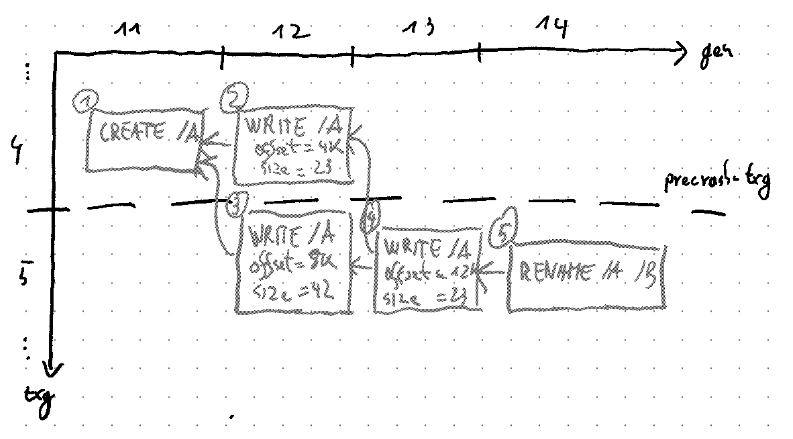
\includegraphics[height=4cm]{fig/prb_logical_structure__diamondchain2}
        \caption{
            The same situation as in Figure~\ref{fig:prb_logical_structure:diamondchain} but entry 4 was written after the precrash-txg.
            Entries 3, 4 and 5 must be replayed.
            If entry 2 is missing, replay would still succeed despite entry 4's dependency on entry 2 because entry 2's effect has already been committed as part of precrash-txg.
            }
        \label{fig:prb_logical_structure:diamondchain2}
    \end{subfigure}
    \caption{
        We visualize the logical log structure as a two-dimensional grid.
        Entries are placed in the grid according to the their generation (x-axis) and transaction group (y-axis).
        The logical dependencies that the log writer expresses through generations are represented as gray directed edges between the entries.
        The \textit{precrash-txg} is represented as a horizontal dashed line.
        The changes in entries above the horizontal line are already applied to the zpool and must not be replayed.
        The changes below the horizontal line need to be replayed.
    }
    \label{fig:prb_logical_structure}
\end{figure}

%Note that a fully sequential chain of entries is sufficient for today's ZIL since the commit list assembled by the ITX code\todo{ref} is already sequential.
%However, as pointed out by the example in the previous paragraph, full sequentiality is not always semantically necessary.
%This observation has already led to a prototype design for ZIL-LWB that allows for more parallel I/O if the entries in written LWBs are not interdependent~\cite{openzfsZILPerformanceImprovements2020}.
%We interpret these findings as indicators that ZIL-PMEM --- and thus PRB --- should support parallelism on the write path in the form of diamond chains.
%We present an application of diamond chains to ZVOLs in Section~\ref{sec:itxgbypass} and evaluate it in Section~\ref{ch:eval}\todo{precise}.

%A generation is identified by its \textit{generation number} which is positive integer.
%An entry is always associated with exactly one generation but a generation can contain many entries.
%Entries within the same generation are identified through an \textit{id field} which is a positive integer.
%Given entries $a$ and $b$, $a \text{depends on} b \Leftrightarrow a.gen > b.gen$ where $x.gen$ denotes the generation of entry $x$.

\subsection{API Overview}\label{di:prb:api} % API Overview?
In this section we provide a guide-level walkthrough of the PRB's API to illustrate the lifecycle of the PRB and HDL.

\subsubsection{PRB Setup}\label{di:prb:api:setup}

\begin{lstlisting}
zilpmem_prb_t* zilpmem_prb_alloc(size_t ncommitters);
void zilpmem_prb_free(zilpmem_prb_t *b, boolean_t free_chunks);

prb_chunk_t *prb_chunk_alloc(uint8_t *pmem_base, size_t len);
void prb_chunk_free(prb_chunk_t *c);

void zilpmem_prb_add_chunk_for_write(
    zilpmem_prb_t *prb, prb_chunk_t *chunk);
void zilpmem_prb_add_chunk_for_claim(
    zilpmem_prb_t *prb, prb_chunk_t *chunk);
\end{lstlisting}

The PRB lifecycle starts during zpool import when we allocate it using the \lstinline{zilpmem_prb_alloc} function.
The returned \lstinline{zilpmem_prb_t} is owned by the caller which is responsible for freeeing it using \lstinline{zilpmem_prb_free} during pool export.

The next step during pool import is to give PRB access to segments of PMEM in the form of \textit{chunks}.
A chunk is a contiguous segment of kernel virtual address space that maps directly to PMEM.
We allocate the chunk using \lstinline{prb_chunk_alloc} and add it to the PRB using either the \lstinline{zilpmem_prb_add_chunk_for_write} or the \lstinline{zilpmem_prb_add_chunk_for_claim} function.
When a chunk is added to the PRB for the first time, we use \lstinline{_for_write}.
Otherwise, e.g. after a system crash, we use \lstinline{_for_claim} to indicate that the chunk needs to be held back for claiming and replay.
The PRB assumes ownership of the chunks that are added to it.
When freeing the PRB using \lstinline{zilpmem_prb_free}, the \lstinline{free_chunks} argument determines whether the chunks are freed immediately or whether ownership moves back to the caller.

The PRB consumer is responsible for ensuring that the PRB is always initialized with the same chunks of PMEM.
We expect the API consumer to partition PMEM into chunks once and to store the partitioning scheme somewhere external to PRB.
In terms of ZIL-PMEM, this means that the PMEM SLOG vdev is partitioned into chunks when it is added to the pool, and that this partitioning does not change until the PMEM SLOG vdev is removed.
In our current implementation we simplify the partitioning by hard-coding a fixed chunk size (\SI{128}{MiB}\todo{check}) and partitioning the PMEM SLOG vdev's allocatable space into contiguous segments of that size.
\todo{future work: dynamically add and remove chunks}

The \textit{ncommitters} parameter to \lstinline{zilpmem_prb_alloc} determines the number of threads that can write to PMEM concurrently.
Since a chunk can only be written by one thread at a given time, at least \lstinline{ncommitters} chunks should be added to the PRB for multi-core scalability.
The value of \lstinline{ncommitters} is also relevant for efficient use of CPU time, as we will elaborate on in Section~\ref{di:prb:write:scalability}.

For robustness against data corruption, it is advisable to limit the size of chunks, i.e., have many more chunks than \lstinline{ncommitters}.
We elaborate on this topic in the Section~\ref{di:prb:recovery} where we describe the algorithms for claiming and replay.

\subsubsection{HDL Setup}\label{di:prb:api:hdl}
\begin{lstlisting}
void zil_header_pmem_init(zil_header_pmem_t *zh);
zilpmem_prb_handle_t* zilpmem_prb_setup_objset(
    zilpmem_prb_t *prb, const zil_header_pmem_t *hdr);
void zilpmem_prb_teardown_objset(zilpmem_prb_handle_t *zph,
    boolean_t abandon_claim, zil_header_pmem_t *upd);
\end{lstlisting}

PRB multiplexes PMEM into many logical logs, one for each ZFS head dataset.
The in-DRAM representation of the per-head dataset state is the HDL (\lstinline{zilpmem_prb_handle_t}).
We instantiate HDLs during pool import or when a new head dataset is created (\lstinline{zilpmem_prb_setup_objset}).
The returned HDL is owned by the caller and can be used to create, write to, replay, and destroy a log.
When the head dataset is destroyed or the pool is exported, we must call \lstinline{zilpmem_prb_teardown_objset} to destroy the HDL.
The PRB cannot be freed before all of its HDL's have been torn down.

In addition to the log entries which are stored in the PMEM chunks, some HDL state needs to be persisted to the main zpool so that log recovery can attribute log entries to the correct log after a crash.
In the context of the ZIL, the natural location for storing this data is the ZIL header due to the 1:1 relationship between head dataset and ZIL chains.
The type that represents serialized HDL state in the ZIL header is the \lstinline{zil_header_pmem_t}.
We cover its exact contents in more detail in Section~\ref{di:prb:persistent}.
For modularity and testability, we split the responsibility of persisting HDL state: whereas the HDL APIs are responsible for serialization, the API consumer is responsible for persistence.
The to-be-persisted update is returned to the API consumer in the form of an out-parameter.
This pattern is used for all HDL-scoped APIs that need to update the ZIL header.
% Whereas PRB unit tests can simply store the ZIL header on the stack, ZIL-PMEM passes a pointer to the in-DRAM dirty copy of the dataset's ZIL header (\lstinline{os_zil_header}).
% After the PRB API function returns, ZIL-PMEM marks the dataset as dirty and waits for the open txg to sync.

\subsubsection{Claiming}\label{di:prb:api:claiming}

\begin{lstlisting}
typedef struct check_replayable_result { ... };

check_replayable_result_t zilpmem_prb_claim(
    zilpmem_prb_handle_t *hdl,
    zil_header_pmem_t *upd,
    uint64_t pool_first_txg);
\end{lstlisting}
% NOTE: we omitted the whole claimstore stuff from the thesis because we rule out WR_INDIRECT support in the 'requirements' section.

After the PRB is constructed and HDLs are set up, we must \textit{claim} log entries to prevent them from getting overwritten until they have been replayed.
For this purpose, \lstinline{zilpmem_prb_claim} must be called in the first transaction group during pool import (\lstinline{pool_first_txg}) for every HDL.
It returns the ZIL header update that records the successful claiming of the HDL's log through the \lstinline{upd} out-parameter.

The \lstinline{zilpmem_prb_claim} function must be called every time the pool is imported, for every dataset.
The reason is that the internal data structure which tracks whether a chunk needs to be held back for replay is only held in DRAM.
\todo{Can't reference chunks in PMEM because they have no explicit repr. But it's also better this way because it minimizes the impact of data corruption in a hypothetical repr.}
\lstinline{zilpmem_prb_claim}'s reconstructs that data structure during pool import by scanning the chunks that were added using \lstinline{zilpmem_prb_add_chunk_for_claim} for replayable log entries.
The data that is used to decide whether a log entry needs to be kept for replay is stored in the per-dataset ZIL header, hence the requirement to invoke \lstinline{zilpmem_prb_claim} for each dataset.

Claiming can fail, e.g., if an entry is lost due to data corruption but is depended upon by other entries.
The API consumer defines the error handling policy.
It can either abort pool import or choose to abandon the log.
To abaondon the log, the API consumer must tear down the HDL using \lstinline{zilpmem_prb_teardown_objset(..., abandon_claim=true, ...)} and set it up again from a freshly initialized header (\lstinline{zil_header_pmem_init}).
\todo{retry with an override flag that discards the unreplayable part of the log}

After we have finished claiming, txg sync writes out the \lstinline{pool_first_txg} and the pool becomes ready for use.
From that point on there is no need to coordinate HDL operations between different datasets.

% Remember from Section~\ref{bg:zfs:logreplay} that ZIL replay can be deferred for an indefinite amount of pool import/export cycles and system shutdowns.
% Claiming scans the PMEM chunks that were added with \lstinline{zilpmem_prb_add_chunk_for_claim} for log entries that need to be replayed.
% Chunks that contain unreplayed log entries are not considered when writing new entries.

\subsubsection{Replay}\label{di:prb:api:replay}

\begin{lstlisting}
typedef struct zilpmem_prb_replay_result { ... }

typedef int (*zilpmem_replay_cb_t)(void *rarg,
    const zilpmem_replay_node_t *rn,
    const zil_header_pmem_t *upd);

zilpmem_prb_replay_result_t zilpmem_prb_replay(
    zilpmem_prb_handle_t *hdl,
    zilpmem_replay_cb_t cb, void *cb_arg);

void zilpmem_prb_replay_done(
    zilpmem_prb_handle_t *hdl,
    zil_header_pmem_t *upd);

typedef enum {
	READ_REPLAY_NODE_OK,
	READ_REPLAY_NODE_MCE,
	READ_REPLAY_NODE_ERR_CHECKSUM,
	READ_REPLAY_NODE_ERR_BODY_SIZE_TOO_SMALL,
} zilpmem_prb_replay_read_replay_node_result_t;

zilpmem_prb_replay_read_replay_node_result_t
zilpmem_prb_replay_read_replay_node(
    const zilpmem_replay_node_t *rn,
    uint8_t *body_out, size_t body_out_size,
    size_t *body_required_size);
\end{lstlisting}

When a dataset is mounted we always replay its log to recover changes that were committed to the application but not synced to the main pool.
The API for this task is \lstinline{zilpmem_prb_replay}.
If there is no log for the dataset or all log entries are obsolete, the function only resets ZIL header.
If there are replayable log entries, it invokes the \lstinline{zilpmem_replay_cb_t} callback for each log entry that needs to be replayed.
The callback must perform the following steps in an single DMU transaction:
\begin{enumerate}[noitemsep]
    \item Apply the change that the log writer encoded in the entry to the dataset.
    \item Record replay progress by updating the ZIL header to the value as a second argument.
\end{enumerate}
Recording replay progress is critical for correctness.
First, it makes replay crash consistent.
If the system crashes during replay, and replay is retried after reboot, the replay algorithm skips entries that have already been applied based on the progress information.
Second, the types of changes that can be encoded in the log need not be idempotent because each change is only applied once.
\todo{feels out of place but this is too much for the overview sections...}

The callback is not given a raw pointer to the log entry in PMEM.
Instead, it must use the \lstinline{zilpmem_prb_replay_read_replay_node} function to read it.
The function ensures that data corruption is handled correctly:
it validates the PRB-managed checksum of the log entry's body and ensures that machine-check exceptions (MCEs) raised\todo{caused?} by PMEM are converted to errors.

\lstinline{zilpmem_prb_replay} can fail either due to an error in the callback or because log entries are missing.
The struct returned by the API contains the log entry that prompted the failure, e.g., the first entry that was missing a logical dependency induced by \textit{generations} (see Section~\ref{di:prb:structure}).
The caller decides whether to retry replay or abandon the remaining unreplayable part of the log\todo{retry with an override flag that discards the unreplayable part of the log}.
End of replay must be acknowledged explicitly by calling \lstinline{zilpmem_prb_replay_done}.
Abandonding the log is done using \lstinline{zilpmem_prb_destroy_log}.

%The invocation order corresponds to the order in which the entries were written.
%Entries that were written in parallel (\lstinline{needs_new_gen == false}) are replayed in a deterministic order to allow for resumability.

\subsubsection{Writing Entries}

\begin{lstlisting}
boolean_t zilpmem_prb_create_log_if_not_exists(
    zilpmem_prb_handle_t *hdl, zil_header_pmem_t *upd);
void zilpmem_prb_destroy_log(
    zilpmem_prb_handle_t *hdl, zil_header_pmem_t *upd);

int zilpmem_prb_write_entry(
    zilpmem_prb_handle_t *hdl,
    uint64_t txg,
    boolean_t needs_new_gen,
    size_t body_len, const void *body_dram);
\end{lstlisting}

After replay, the HDL is in a state that requires creation of a new log in order to write log entries.
We use the \lstinline{zilpmem_prb_create_log_if_not_exists} to perform this task idempotently.
The return value indicates whether a header update is actually necessary.

We use the \lstinline{zilpmem_prb_write_entry} function to write \textit{log records} to the created log.
As explained in Section~\ref{di:prb:structure}, PRB treats log records as opaque blobs that encode a logical change to the dataset.
The log writer and callback must agree on an encoding before writing log entries or replaying them from the PRB.
PRB does not provide facilities to version different version of the encoding.\todo{fix in upstream release?}

In addition to the encoded log record (\lstinline{body_dram}, \lstinline{body_len}), the log writer must provide two pieces of metadata:
\begin{description}[noitemsep,leftmargin=1.5cm,labelindent=1cm]
    \item[txg] The transaction group $T_{i_{txg}}$ of the DMU transaction $T_i$ whose changes $C_i$ are encoded in the log entry (Section~\ref{di:prb:structure}).
        During normal operation, the value is used by garbage-collection to identifiy obsolete log entries.
        During claiming and replay, the value is used to determine whether the entry needs to be replayed.
        Note: for ZIL-PMEM, this value is always the same as the log record's \lstinline{lrc_txg} field.
    \item[needs\_new\_gen] Indicates whether a new generation should be started for this log entry (Section~\ref{di:prb:structure}).
        It is the responsiblity of the caller to serialize the start of a new generation:
        if a thread writes an entry with \lstinline{needs_new_gen} is \lstinline{true}, that thread must be the only thread executing \lstinline{zilpmem_prb_write_entry} for the given HDL.
        The inverse\todo{contrary?} is not true: if \lstinline{needs_new_gen} is \lstinline{false}, multiple threads may write entries in parallel to the same HDL.
        Note that writers for different HDLs need not coordinate at all.\todo{language?}
\end{description}

\subsubsection{Garabge Collection}

\begin{lstlisting}
void zilpmem_prb_gc(zilpmem_prb_t *prb, uint64_t synced_txg);
\end{lstlisting}

Whenever \textit{txg sync} has finished syncing a txg $T$ to the main pool it must call \lstinline{zilpmem_prb_gc} with \lstinline{synced_txg == T}.
The function makes chunks available for writing that are full and only contain log entries written for txgs older \lstinline{synced_txg}.
Note that unlike writing or recovering an individual log, garbage collection is a PRB-level operation.
It is safe to call \lstinline{zilpmem_prb_gc} without synchronization with HDL-level APIs.

\subsection{Persistent Data Structure}\label{di:prb:persistent}
In this section we describe how we persist PRB to stable storage.
The state that must be persisted is the content of each HDL's logs and the HDL state that is necessary for claiming and crash-consistent replay.
Our basic design principle is the decoupling of storage location and logical log structure.
Separating these concerns allows us to optimize the write path (Section~\ref{di:prb:write}) for latency at the expense of some complexity during recovery (Section~\ref{di:prb:recovery}).

The persistent state is comprised of the following entities:
\begin{description}[noitemsep,leftmargin=1.5cm,labelindent=1cm]
    \item[PMEM chunks] The segments of contiguous PMEM space that are added to the PRB during setup (see Section~\ref{di:prb:api:setup}).
    \item[Entry] The representation of a log entry. It consists of PRB-managed metadata and the actual log record data provided by the PRB API user.
    \item[ZIL Header] The persistent representation of a subset of HDL state that is relevant for recovery.
\end{description}
In the remainder of this section we describe the structure of these entities and how they relate to each other.
Figure~\ref{fig:prb_physical_data_structure_entities} puts everything together in a visual summary.\todo{language, ideas welcome}

\begin{figure}
    \centering
    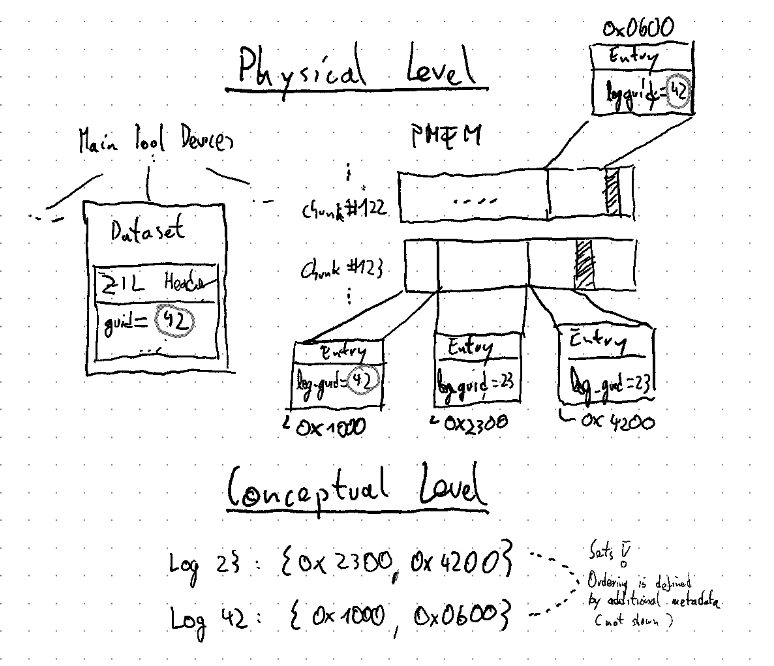
\includegraphics[height=8cm]{fig/prb_physical_data_structure_entities}
    \caption{
        The relationships between the different entities that constitute PRB's persistent state.
    }
    \label{fig:prb_physical_data_structure_entities}
\end{figure}

% \begin{description}
%     \item[Space-Multiplex PMEM] The PMEM space in the chunks added to the PRB must be shared among all HDLs.
%     \item[Crash Consistent Writes] Writing entries to a HDL must at no point in time cause loss of existing entries.
%     \item[Data Integrity] Entries must be stored such that data corruption can be detected using an error-detecting code.
%     \item[Parallel Writes] 
%     \item[Garbage Collection] The space occupied by entries that are obsoleted by txg sync must be freed by the PRB-wide garbage collection callback.
% \end{description}

\subsubsection{Chunks}\label{di:prb:persistent:chunks}
PRB stores log entries in the PMEM chunks that were assigned to it.
As explained in the API walkthrough (Section~\ref{di:prb:api:setup}), it is the PRB API consumer's responsibility to deterministically partition PMEM into segments, allocate \lstinline{prb_chunk_t} DRAM objects, and add them to the PRB during pool import.
Therefore, PRB does not need to define persistent structures that track the PMEM partitioning.
From PRB's perspective, chunks are mere slices of PMEM defined by a \textbf{base address} and \textbf{length} value.
The base address is allowed to change every time the PRB is instantiated as long as the effective PMEM space that it refers to remains the same.
Due to Intel Optane-specific performance characteristics, we require that the base address must be aligned to 256 bytes and that the length in bytes must be a multiple of 256.
We will elaborate on this requirement in Section~\ref{di:prb:di:prb:write:crashconsistency}\todo{check}.

Chunks act as containers for \textit{entries}.
They are stored within the chunk's PMEM slice as a contiguous sequence, starting with the first entry at the base address.
The space after an entry is zero-padded to the next multiple of 256 bytes.
The next entry starts after the padding.
The sequence is terminated either explicitly by an invalid entry header or implicitly if the last entry has filled the chunk completely.
Figure~\ref{fig:prb_physical_data_structure__chunklayout} provides an example chunk layout.

Note that chunks must be sufficiently large to hold at least one entry because entries cannot be split across chunks.
The choice of chunk size is a trade-off between PMEM space-efficiency (fragmentation at the end of the chunk), the acceptable blast radius\todo{this is a common ops term but not sure if academic enough...} of data corruption (traversal, see Section~\ref{di:prb:traversal}), and multi-core scalability on the write path (see Section~\ref{di:prb:write}).

\begin{figure}[h]
    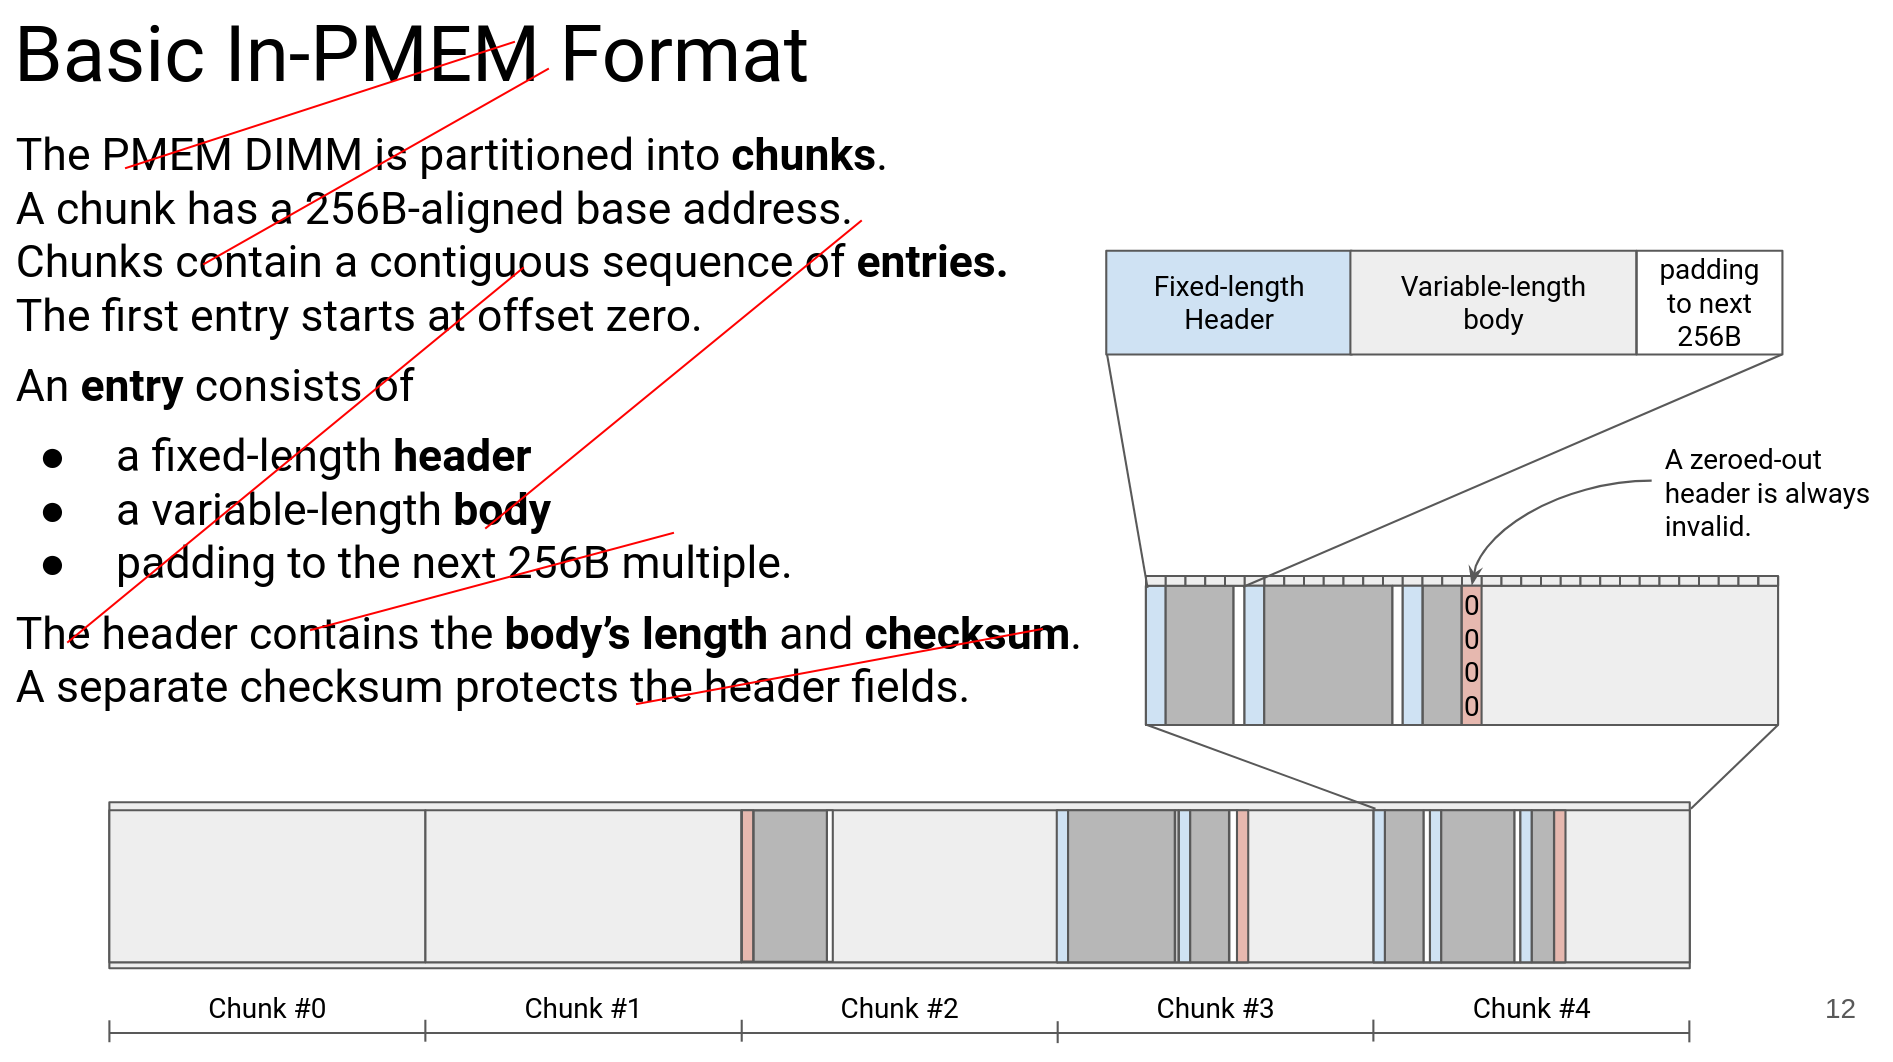
\includegraphics[height=7cm]{fig/prb_persistent_structure__chunklayout}
    \caption{Example chunk layout. Note that although we partition the PMEM space very regularly in this example, the PRB consumer is free to use variable-sized chunks.}
    \label{fig:prb_physical_data_structure__chunklayout}
\end{figure}

\subsubsection{Entry}\label{di:prb:persistent:entry}
Log entries are represented as a fixed-length header and a variable-length body as visualized in Figure~\ref{fig:prb_physical_data_structure__chunklayout}.
The body is a verbatim copy of the byte slice passed to \lstinline{zilpmem_prb_write_entry}.
The header's contents are managed by the PRB implementation.
It stores metadata that allows the recovery procedures to
\begin{itemize}[noitemsep]
    \item iterate over the entry sequence stored in the chunk,
    \item ensure data integrity,
    \item attribute entries to a given HDL's log, and to subsequently
    \item determine the set and order\todo{weird language, how to phrase this?} of entries that need to be replayed (see Section~\ref{di:prb:structure}).
\end{itemize}

The following metadata enables \textbf{iteration} over the entries in a chunk:
\begin{description}[noitemsep,leftmargin=1.5cm,labelindent=1cm]
    \item[Body Length] We store the exact body length in bytes. The zero padding in the chunk sequence is not considered part of the entry itself.
    \item[Header Checksum] The header checksum ensures data integrity of the metdata. It is used to detect data corruption and torn writes.
    If the header checksum is corrupted the header fields cannot be trusted, including the body length.
    We use ZFS's optimized implementation of the Fletcher 64bit checksum.
\end{description}
We outline the algorithm for traversal in Section~\ref{di:prb:traversal}.

In order to ensure \textbf{end-to-end data integrity} for the payload stored in the entry body, we use a separate checksum.
\begin{description}[noitemsep,leftmargin=1.5cm,labelindent=1cm]
    \item[Body Checksum] Fletcher 64bit checksum of the body data.\todo{parametrize checksum algorithm, store in HDL?}
\end{description}

We \textbf{attribute} entries to a given HDL's log through the \textit{log GUID}:
\begin{description}[noitemsep,leftmargin=1.5cm,labelindent=1cm]
    \item[Log GUID] A 128 bit random identifier stored in the HDL's ZIL header and repeated in every entry written through that HDL.
\end{description}

Claiming and replay use the following data to determine which entries need to be replayed and the order in which that must happen:\todo{also not great language...}
\begin{description}[noitemsep,leftmargin=1.5cm,labelindent=1cm]
    \item[Transaction Group (txg)] The transaction group in which the change encoded in the entry was or would have been synced out by \textit{txg sync}.
        The value is provided as an argument to \lstinline{zilpmem_prb_write_entry} by the log writer.
    \item[Generation Number (gen)] We represent generations as unsigned 64-bit non-zero integers.
        The ordering of the generations in the log is given by the ordering of the generation numbers.
        Thus, whenever a new generation is started, its generation number must be greater than any previously used generation number for that log.
        Overflow of the generation must be handled in software, e.g., by starting a new log.
        Note that our design does not handle overflow because even with the (absurdly) conservative of \SI{1}{ns} write time per log entry, the first overflow event would only occur in \SI{584}{years}.
        %When a log is created the generation number starts at $1$.
        %When an entry is written, the log's current generation number is stored in the entry header.
        %If the log writer requests that the log entry be placed in a new generation, the generation number is incremented.
        %There are no provisions for wrap-around.
    \item[Generation-Scoped ID (gsid)] Within a generation, we identify and order entries by a unique unsigned 64-bit non-zero integer.
        As the name suggests, the gsid only need to be unique within a generation.
    \item[Counters Table] Each entry contains a table that stores the number of entries that have been written up to generation $gen$, by transaction group.
        Only the counters for transaction groups $txg$, $txg - 1$, and $txg - 2$ are stored in the table.
\end{description}
Note that the Counters Table is the same for all entries in a generation because, by the definition above, it does not count the entries of the open generation at the time the entries are written.
%We currently replicate it in each entry to minimize coordination between parallel writers.
%The Counters Table is critical for detecting missing entries during claiming and replay (Section~\ref{di:prb:recovery}).

\subsubsection{ZIL header}\label{di:prb:persistent:zilheader}
The ZIL header (\lstinline{zil_header_pmem_t}) is the persistent representation of the HDL state.
Not every aspect of the runtime state of HDL is reflected in it, but only the information needed for claiming and replay.
The ZIL header has the following states, some of which have associated data:
\begin{description}[noitemsep,leftmargin=1.5cm,labelindent=1cm]
    \item[nozil] There is no log for this dataset. (No associated data.)
    \item[logging] The log has been created and entries might have been written to PMEM.
        Claiming has never been attempted or never been completed.
        The log remains in this state for the entire time until it is destroyed or the system crashes. Associated data: \textit{Log GUID}.
    \item[replaying] The log has been claimed and replay is ongoing. Associated data: \textit{Log GUID} and \textit{serialized replay algorithm state}.
\end{description}
The diagram in Figure~\ref{fig:prb_persistent_structure__header_states_plus_example} visualizes the state transitions that the ZIL header goes through as the log is created, written and recovered.

\begin{figure}
    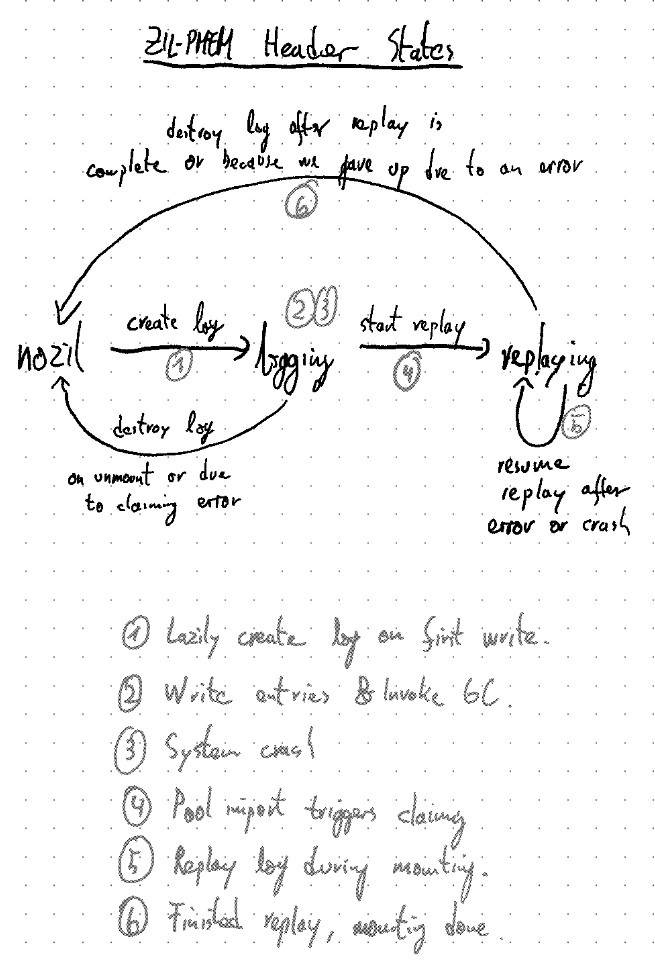
\includegraphics[height=15cm]{fig/prb_persistent_structure__header_states_plus_example}
    \caption{
        The states of \lstinline{zil_header_pmem_t} and the events that cause state transitions.
        The grey annotations illustrates the path from log creation to finished recovery.}
    \label{fig:prb_persistent_structure__header_states_plus_example}
\end{figure}

We use the following C structure to encode the ZIL header state.
The \lstinline{zhpm_st} field is always valid and is one of \lstinline{ZHPM_ST_NOZIL}, \lstinline{ZHPM_ST_LOGGING}, or \lstinline{ZHPM_ST_REPLAYING}.
The \lstinline{zhpm_guid_} fields are only valid in states \lstinline{ZHPM_ST_LOGGING} and \lstinline{ZHPM_ST_REPLAYING}.
The \lstinline{zhpm_replay_state} is only valid in state \lstinline{ZHPM_ST_REPLAYING}.
Hence we will describe its contents in Section~\ref{di:prb:recovery}.
\begin{lstlisting}
typedef enum zil_header_pmem_state {
    ZHPM_ST_NOZIL,
    ZHPM_ST_LOGGING,
    ZHPM_ST_REPLAYING,
} zil_header_pmem_state_t;

typedef struct zil_header_pmem {
    uint64_t zhpm_st; /* zil_header_pmem_state_t */
    uint64_t zhpm_guid_1;
    uint64_t zhpm_guid_2;
    zilpmem_replay_state_phys_t zhpm_replay_state;
} zil_header_pmem_t;
\end{lstlisting}


\subsection{Traversal}\label{di:prb:traversal}
As described in the previous section\todo{check ref}, PRB stores entries in chunks as a contiguous sequence.
In this section we describe the algorithm that is used to iterate over the entries in that sequence.

As a reminder, the data layout within the chunk is as follows:
\begin{itemize}[noitemsep]
    \item The first entry header starts at chunk offset zero. Its size is fixed (256 bytes).
    \item The variable-length body starts immediately after the header. Its length is stored in the header.
    \item The body is followed by zero padding to the next 256 byte multiple.
    \item The next entry's header starts there.
    \item An invalid header marks the end of the chain. For example, a zero \textit{log GUID} is defines as invalid.
    \item Entries are never split between chunks.
\end{itemize}

In the absence of data corruption in PMEM, it is guaranteed that every entry in the sequence is visisted.
In the presence of data corruption, we distinguish several cases:
\begin{description}
    \item[Machine check exception (MCE)] If the PMEM hardware detects uncorrectable data corruption, it raises an MCE.
        We use the Linux kernel's \lstinline{memcpy_mcsafe} function that converts such exceptions into error values.
        The error handling for MCE errors is the same as for invalid checksums in entry header and body, which we describe below.
    \item[Header checksum detects corrupted header]
        If the header checksum validation fails, the header was either corrupted by bitflitps or similar phenomena or never completely written.
        The latter case is critical for crash consistency on the write path as we will elaborate on in Section~\ref{di:prb:write:crashconsistency}.
        Regardless of the cause, an invalid header's values cannot be trusted, and thus the traversal stops.
    \item[Header checksum does not detect corrupted header]
        If the header checksum does not detect data corruption in the header, the behavior is implementation-defined.
        However, it is guaranteed that memory accesses are constrained to the entry's chunk's bounds.
    \item[Data corruption in the body]
        The traversal algorithm does not read the body but instead returns a closure that can be invoked for this purpose.
        The closure reads the body into DRAM using \lstinline{memcpy_mcsafe}, then validates the body checksum stored in the header.
        Validation failures are returned as an error.
        The caller can decide whether they want to iterate further or propagate the error up the call stack.
        Note that in our C implementation, the closure is replaced by the opaque struct \lstinline{zilpmem_replay_node_t} and function \lstinline{zilpmem_prb_replay_read_replay_node}.
    \item[Data corruption in the padding]
        We require that the padding in the space that follows the body to the next 256 byte multiple consists only of zero.
        We validate this property in the closure that reads the body.
        Validation failure results in a distinguished error being returned from the closure.
        Such an error is indicative of data corruption or an incorrect implementation on the write path.
        The caller of the traversal algorithm should surface it to the administrator, but may choose to proceed.
\end{description}

The following listing provides pseudo code for chunk iteration.
\begin{lstlisting}
Algorithm: iter_chunk() - Iterate over the entries in a chunk.

Inputs:

    ch_base    chunk's base address
    ch_len     chunk's length

Procedure:
    assert ch_base % 256 == 0
    assert ch_len >= sizeof(entry_header_t)
    assert ch_len % 256 == 0

    e := ch_base
    while (e < ch_base + ch_len) {
        entry_header_t eh;

        // read header with a function that handles machine-check exceptions
        memcpy_mcsafe(&eh, e, sizeof(eh))?;

        validate_header_checksum(eh)?;

        if eh.log_guid == 0 {
            // invalid header terminates the sequence
            return None;
        }

        body_ptr := e + sizeof(eh);

        if body_ptr + eh.body_len > ch_base + ch_len {
            return Err("entry out of chunk boundary:"
                    "a) writer implementation error "
                    "b) undetected header corruption "
                );
        }
        e += sizeof(eh) + body_len;
        e = roundup_to_next_256byte_multiple(e);

        padding_ptr := body_ptr + eh.body_len
        padding_len := e - padding_ptr

        read_body := |buffer: *u8| {
            memcpy_mcsafe(buffer, body_ptr, eh.body_len)?;
            validate_body_checksum(eh, buffer, eh.body_len)?;
            pmem_is_zero(padding_ptr, padding_len)?;
            return Ok(());
        };
        yield Some((eh, read_body))

    }

Example:

    for (entry_header, read_body) in iter_chunk(ch_base, ch_len) {
        if entry_header.txg <= precrash_txg {
            continue;
        }
        buf := buffer of size entry_header.body_len
        read_body(buf)?;
        ...
    }
\end{lstlisting}

\subsection{Chunks \& Chunk Ownership}\label{prb:di:chunkownership}
% In this section we provide an overview of the in-DRAM data structures used by PRB and HDL.
% PRB is represented by the \lstinline{zilpmem_prb_t} structure.
% It acts as the root for all PRB-related runtime state.
% \begin{description}
%     \item[HDL Tree] PRB tracks HDLs in a search tree for their entire in-DRAM lifetime (\lstinline{zilpmem_prb_setup_objset} and \lstinline{zilpmem_prb_teardown_objset}).
%     The search tree is used to enforce API contracts, e.g., that a HDL must only be \lstinline{setup} once and that all HDLs must have been torn down before the PRB is freed.
%     \item[Per-HDL State] Each HDL 
%     The HDLs themselves have internal state with associated data. 
%     The state stored within the HDLs is specific to the write path and recovery  is only relevant during replay and will thus be presented in the corresponding Section~\ref{di:prb:recovery}.
%     \item[Chunk Ownership: Chunk Lists \& Commit Slots] PRB needs  uses chunks to allow as the  tracks chunk ownership  the chunks that were assigned to it during construction in a set of lists.
%     We describe commit slots below.
% \end{description}

% \subsubsection{Chunks}
Each chunk in PMEM is represented by a corresponding \lstinline{prb_chunk_t} DRAM object that is allocated by the PRB API consumer during PRB construction.
Each chunk object has the following runtime state:
\begin{description}[noitemsep]
    \item[PMEM location] The chunk's start and end address in PMEM. These values do not change for the lifetime of the chunk.
    \item[Claim refcount] Each HDL that requires one or more entries in the chunk for replay must hold a reference to the HDL so that garbage-collection skips the chunk.
        HDLs add references during claiming and remove them after replay is complete or the log is abandoned.
    \item[Write position] The PMEM address where the next entry will be written. The value is reset to the chunk's start address by garbage collection.
    \item[Max txg] The maximum transaction group of the entries that were written to this chunk. The value is reset to zero by garbage collection.
\end{description}

% \subsubsection{Chunk Ownership}\label{prb:di:chunkownership}
We use an ownership model to define which entity is allowed exclusive access to a chunk's state, both in DRAM and in PMEM.
Initially, the chunk is owned by the API consumer that allocated it.
When the API consumer adds the chunk to the PRB, ownership of the chunk moves to the PRB until the PRB is freed.
Within the PRB, the chunk is either put on one of several lists or it is held by a \textit{commit slot}.
A commit slot can hold at most one chunk at any given time.
When a log write wants to write an entry it first \textit{aquires} a commit slot and then writes the entry to the commit slot's chunk.
All chunks that are not owned by a commit slot are tracked in exactly one of the following lists:
\begin{description}[noitemsep]
    \item[Free List]
        The \textit{free list} holds empty chunks.
        Their \textit{claim refcount} and \textit{max txg} is zero and their write position is reset to the chunk's base address.
        In PMEM, the entry sequence is empty because the entry header at the chunk's base address is invalid.
        The list is filled by \lstinline{zilpmem_prb_add_chunk_for_write} and from garbage collection.
        It is used by log writers that cannot fit their entry into their commit slot's current chunk:
        the log writer puts the commit slot's current chunk on the \textit{full list} (see below) and gets a new chunk from the \textit{free list}.
    \item[Full Lists]
        The \textit{full lists} contains chunks that wait for garbage collection.
        PRB maintains one full list for each txg $T_i$. The \textit{full list} for $T_i$ contains exactly those chunks whose \textit{max txg} is $T_i$.
        When \textit{txg sync} triggers garbage collection for $T_i$, the chunks on the corresponding \textit{full list} are reset and moved to the \textit{free list}.
        Note that it is sufficient to maintain three full lists at any given time --- one for each of the three unsynced transaction groups \textit{open}, \textit{quiescing}, and \textit{syncing}.
        The three lists can be represented as an array of three lists that is indexed by $T_i \mod 3$.
        The implementation follows the common ZFS idiom of using four lists that are indexed by \lstinline{T_i&3} where \lstinline{&} is the \textit{bitwise and} operation.
        \todo{ref central explainer for this}
    \item[Wait Replay List]
        The \textit{wait replay list} contains the chunks that were added to the PRB using \lstinline{zilpmem_prb_add_chunk_for_claim}.
        When a HDL log is claimed, the claiming procedure scans the chunks on this list and increments the \textit{claim refcount} for chunks that need to be kept.
        Once claiming is done and \textit{txg sync} triggers the first garbage collection cycle after pool import, any chunk on this list that has a zero refcount is reset and moved to the \textit{free list}.
        The list is also scanned for zero refcounts during all future garbage collection cycles.
\end{description}
We visualize the ownership transitions in Figure~\ref{fig:prb_chunk_ownership_cycle__transitions} and provide an example in Figure~\ref{fig:prb_chunk_ownership_cycle__example}.

\begin{figure}[H]
    \centering
    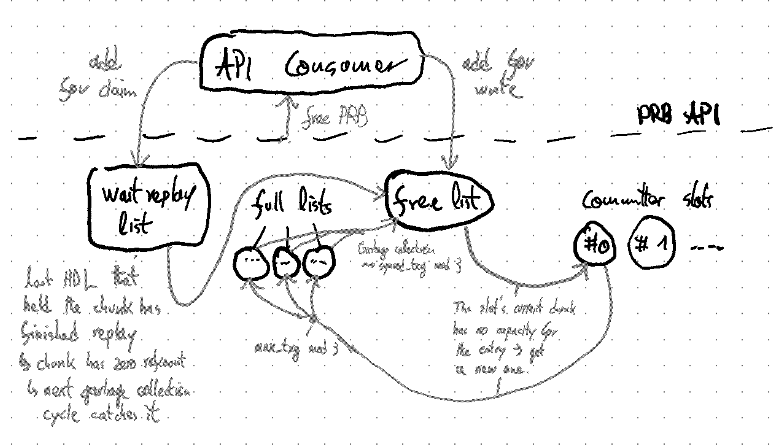
\includegraphics[width=\textwidth]{fig/prb_chunk_ownership_cycle__transitions}
    \caption{The different owners of a chunk and the events that cause ownership transitions.}
    \label{fig:prb_chunk_ownership_cycle__transitions}
\end{figure}

\begin{figure}[H]
    \centering
    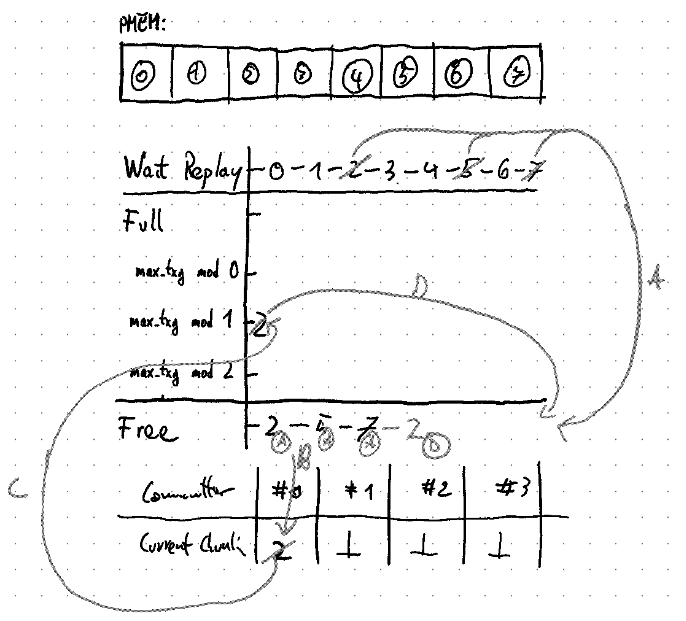
\includegraphics[height=12cm]{fig/prb_chunk_ownership_cycle__example}
    \caption{
        Example for chunk ownership transitions.
        The PRB is constructed with all eight chunks added as \lstinline{_for_claim}.
        Claiming (\textit{A}) determines that chunks 0, 1, 3, 4, and 6 need to remain on the \textit{wait replay list} because they contain entries for HDL logs that need replay.
        Chunks 2, 5, and 7 only contain obsolete entries and move to the \textit{free list}.
        We do not replay any of the logs.
        However, a log writer starts writing a new log in \textit{B}.
        It finds that its commit slot (\#0) has no active chunk.
        Thus, it and moves the first chunk on the \textit{free list} (i.e., chunk 2) to the commit slot.
        After writing the entry to chunk 2 the log writer releases the commit slot.
        Another log writer aquires commit slot \#0 and writes entries to it.
        Chunk 2's capacity is insufficient to hold the last entry (\textit{C}).
        The thread places chunk 2 on the correct \textit{full list} for chunk 2's \textit{max txg} and finds a new chunk on the free list for the commit slot (not shown).
        Eventually \textit{txg sync} triggers garbage collection for the txg that is chunk 2's \textit{max txg} which resets chunk 2's in-PMEM and in-DRAM sequence and subsequently places it back onto the free list.
    }
    \label{fig:prb_chunk_ownership_cycle__example}
\end{figure}

\subsection{Write Path}\label{di:prb:write}
In this section we present the design and implementation techniques that we employ to persist log entries in PMEM.
Our primary goal is performance: we want our design to minimize PRB's latency overhead and maintain this property for parallel writers on a multicore system.
At the scope of PRB (not ZIL-PMEM as a whole), the following activities on the write path are relevant for latency:
\begin{description}[noitemsep]
    \item[Checksumming] We must compute the Fletcher checksums of the header and body for each log entry that is being written.
        This task adds latency but does not concern multicore scalability since no coordination is required between writers.
    \item[Log Structure Encoding] We must compute the \textit{Counters Table} every time a log writer starts a new generation.
        As the name indicates, we must maintain a precise counter of the number of log entries that were written for each txg.
        The Counters Table and thus the counters are private to each log.
        It only presents a scalability concern for parallel writing to the same log, which is not the case for ZIL-PMEM proper but relevant for our ZVOL-specific ITXG bypass (Section~\ref{sec:itxgbypass}).
        \todo{linux percpu counter precise?}
    \item[Commit Slot Aquisition \& Chunk Replacement]
        A thread that writes a log entry must aquire a commit slot and might need to replace its commit slot's current chunk if its capacity is insufficient.
        These concerns present multicore-scalability challenges since both commit slots and the chunk lists are PRB-wide state that requires coordinated access.
    \item[Crash Consistency] The procedure that appends the log entry to the target chunk's sequence must do so in a crash-consistent manner.
        This typically requires the insertion of store barriers for correctness and comes with a latency cost.
    \item[Optane-Specific Performance Characteristics]
        We develop and evaluate ZIL-PMEM for/on Intel Optane DC Persistent Memory.
        The performance characteristics of Optane DIMMs are significantly different from regular DRAM.
        For example, the access granularity and kind of store and cache flush instruction have significant impact on the achievable write bandwidth~\cite{yangEmpiricalGuideBehavior2020}.
        \todo{need background section for pmem characteristics papers?}
\end{description}
The secondary goal for the write path is the efficient use of CPU time. This concerns the following domains:
\begin{description}[noitemsep]
    \item[Checksumming] Use ZFS's optimized implementations of the Fletcher checksum to compute the entry header and body checksum.
    \item[Writing Entries] Use AVX512 non-temporal store instructions for writing log entries to PMEM.
        For the size of log entries written by ZIL-PMEM, this is the recommended technique by \citeauthor{yangEmpiricalGuideBehavior2020} \cite{yangEmpiricalGuideBehavior2020}.
    \item[PMEM Bandwidth Limits \& Multicore Scalability] The PMEM programming model dictates that I/O wait time is spent on-CPU --- typically at a memory barrier instruction or because the CPU has exhausted its store or load buffer capacity\todo{review terminology; need proof?}.
        This is problematic from a CPU utilization perspective.
        For example, if multiple threads attempt to write at higher bandwidth than PMEM can sustain, they still appear busy towards the OS thread scheduler and waste CPU time that could be used more productively by other threads in the system.
        \citeauthor{yangEmpiricalGuideBehavior2020} have shown that a single Optane DIMM's write bandwidth can be exhausted by one CPU core at \SI{2}{GB/s}.
        Write bandwidth decreases to \SI{1}{GB/s} at ten or more concurrently writing CPU cores ~\cite{yangEmpiricalGuideBehavior2020}.
        Whereas excessive on-CPU waiting might be the right trade-off in certain userspace applications of PMEM, a kernel file system such as ZFS cannot make assumptions about the system's overall CPU priorities.
        We expect that PMEM write bandwidth can be exhausted in real-world use cases for ZIL-PMEM.
        Our design must therefore find a way to limit concurrent access to PMEM and shift PMEM wait time off the CPU.
\end{description}
%Finally, we want to address the limitations of our design as declared in Section~\ref{sec:requirements}.
%\begin{description}[noitemsep]
%    \item[No Encryption] We do not OpenZFS native encryption. If we did, it would affect software latency and CPU efficiency in the same way the to the checksumming does.
%    \item[No Protection Against Scribbles] Low-latency mechanisms to protect against scribbles have been presented in prior work. We would not expect a significant latency impact.
%    \item[No Data Redundancy] Latency overheads would have to be expected if this feature were added in the future.
%    \item[No Software Striping Of PMEM] We would expect latency overhead with this feature because access to striped PMEM would need to be coordinated.
%        However, Intel Optane's hardware striping seems promising.
%    \item[No Support for WR\_INDIRECT] Support for \lstinline{WR_INDIRECT} records would incur significant latency cost due to the wait time for the main vdevs in the pool.
%    \item[Space Efficiency] 
%\end{description}

In the remainder of this section we present our design and describe how it addresses the challenges listed above.
%We take a top-down approach, starting with an overview of the high-level control flow in Section~\ref{di:prb:write:controlflow}.
%In Section~\ref{di:prb:write:chunksel} we describe how 
%In Section~\ref{di:prb:write:logstructureencoding} we present the algorithm that is used to compute the Counter Tables for each new generation.
% ...

\subsubsection{High-Level Overview}\label{di:prb:write:controlflow}
A thread that writes an entry first aquires a \textit{commit slot} which is our mechanism to limit concurrent writes to PMEM.
Afterwards, it updates the structure that is used to compute the Counter Table.
If the thread is starting a new generation, this step also involves the computation of the new Counter Table.
The next step is to select a suitable PMEM chunk. Whereas the commit slot's current chunk is preferred, we might need to get a new chunk if its space is insufficient.
After a suitable chunk has been selected, we can write the entry.
First we must temporarily disable preemption and saving of FPU context to enable the use of AVX-512.
Next, we compute the Fletcher checksum of the entry body and header.
Finally, we append the entry to the sequence stored in the chunk in a crash-consistent manner.

\begin{figure}[H]
    \centering
    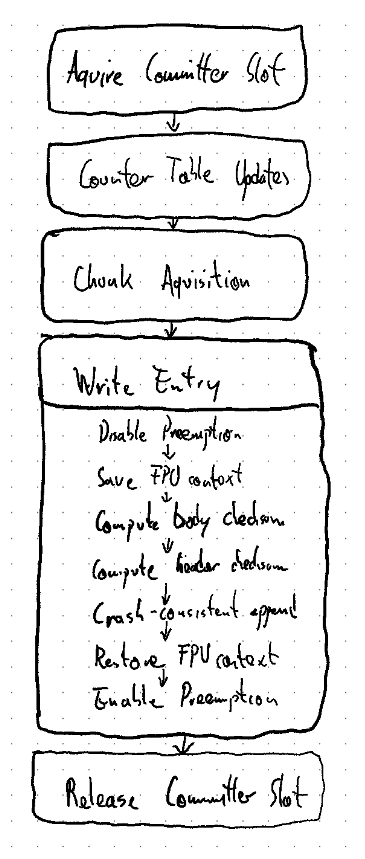
\includegraphics[height=10cm]{fig/prb_writepath_highlevel_activity_diagram}
    \caption{Overview of the steps that are taken on the write path.}
\end{figure}

\subsubsection{Commit Slots}\label{di:prb:write:chunksel}
The commit slot abstraction is our solution to coordinate access to PMEM among multiple parallel writers.
The goal is to allow up to \lstinline{ncommitters} threads simultaneous access to PMEM.
For this purpose, a thread that wants to write an entry \textit{aquires a commit slot} $S \in {0, 1, \dots, ncommitters-1}$.
Each thread that is simultaneously committing gets a different commit slot.
The function to aquire a commit slot blocks the calling thread until a commit slot is available.

A commit slot can hold up to one chunk.
A thread that aquires a commit slot assumes temporary ownerhsip of the associated chunk.
The thread can write its entry to the chunk or replace the chunk with a new one if the chunk's capacity is insufficient.
To replace a chunk, the thread aquires a PRB-wide mutex, then puts chunk on the correct \textit{full list} and gets a new chunk from the \textit{free list}.
Dequeuing a chunk from the \textit{free list} fails if there are no free chunks.
The log writer can choose whether to block and wait or fail the log entry write operation with an error.
Block-and-wait is implemented through a condition variable that is signalled from garbage collection.

If the log writer chooses to block and wait during chunk replacement, it must guarantee that it does not prevent \textit{txg sync} from making progress in order to avoid a pool-wide deadlock.
In practice, this means that the log writer must not hold a DMU transaction open when writing an entry.
Note that this is the case for ZIL-PMEM proper because \lstinline{zil_commit} is called after the DMU transactions have finished or failed.
However, for the ITXG bypass for ZVOLs (Section~\ref{sec:itxgbypass}\todo{chapter?}), we write log entries from within the DMU transaction and thus need to use the non-blocking mode.
\todo{maybe we should change the design to always use non-blocking?}

We implement commit slots using a semaphore and a bitmask.
The aquiring thread must enter the semaphore first, then aquire a slot by finding a zero bit in the \lstinline{ncommitters} least significant bits of the bitmask.
We use atomic compare-and-swap operation and GCC's \lstinline{__builtin_ffs} function to find and flip a zero bit in the bitmask.
We retry indefinitely if the compare-and-swap operation detects a race with another thread.
While this technique does not guarantee a bounded waiting time, we found it to not be problematic in practice in our evaluation.\todo{we have the dtrace probe, but I think we don't have an automated benchmark for this yet.}
The following listing describes the algorithm for commit slot aquisition and release.

\begin{lstlisting}
typedef struct zilpmem_prb {
    ...
    size_t ncommitters; /* immutable */
	semaphore_t committer_sem;
	uint64_t committer_slots;
    ...
} zilpmem_prb_t;

size_t aquire_committer_slot(zilpmem_prb_t *prb) {

    < aquire prb.committer_sem >

    // get a snapshot of prb->committer_slots
	uint64_t committer_slots;
	const uint64_t ncommitters_mask = (1ULL << prb->ncommitters) - 1;
	committer_slots = atomic_load(&prb->committer_slots);

	while (true) {

        // find first set bit on the inverted committer_slots snapshot
		int idx_plus_1 = __builtin_ffs(~committer_slots);
		int idx = idx_plus_1 - 1;
		const uint64_t slot_mask = (1ULL << idx);
		bool won = compare_exchange(
            ptr: &prb->committer_slots,
            expect: &committer_slots,
            updated: committer_slots | slot_mask
        );

		if (won) {
			return idx;
		} else {
            // Ee lost the race with another thread.
            // committer_slots contains the updated value.
            // retry
        }

	}
}

void release_committer_slot(zilpmem_prb_t *prb, size_t slot)
{
    // set the `slot` bit in the bitmask to zero
	const uint64_t slot_mask = 1ULL << slot;
	atomic_and(&prb->committer_slots, ~slot_mask);

    < release prb->committer_sem >
}
\end{lstlisting}

\subsubsection{Counter Table}\label{di:prb:write:logstructureencoding}
The Counters Table is used by claiming and replay (Section~\ref{di:prb:recovery}) to detect missing log entries in a log.
For an entry in generation $G$, it contains the number of entries that were written to the log since the log was created until generation $G$ started.
The entries are counted in separate counters $C_t$ for each transaction group:
if an entry $E$ is written in generation $G$ for transaction group $T$, the counter $C_T$ in the Counters Table of generation $G+1$ is incremented by one.

It is sufficient to include only those counters $C_{t_{u}}$ in the Counters Table whose transaction groups $t_u$ have not yet been synced by txg sync.
The reason is that log recovery only checks for missing log entries in unsynced transaction groups; changes in synced transaction groups will not be replayed and their corresponding log entries might have already been garbage collected.
We conservatively approximate the values for $t_u$ based on the log entries that were written in previous generations.
Assume that $N$ log entries $E_i$ for transaction groups $T_i$ have been written to a log $L$ in generations $G_i < G$.
Then $t_{max} := \max \{ T_i : i \in 1 \dots N \}$ is the youngest transaction group in which an entry was logged to $L$ in generations $G_i$.
Let us (most conservatively!) assume that $t_{max}$ is still the \textit{open} transaction group among the three possible unsynced transaction groups (\textit{open}, \textit{quiescing}, \textit{syncing}).
Then a conservative approximation of the transaction groups that contain changes whose entries were logged to $L$ in generations $G_i$ is $\{ t_{max}, t_{max}-1, t_{max}-2 \}$.

Our implementation uses two separate tables per HDL.
The first table (\textit{live table}) contains the counters that are updated as new entries are being written.
The second table (\textit{last table}) is the Counters Table for the entries that are being written.
It is computed from the state of the \textit{live table} when the currently open generation was started.

We represent the \textit{live table} as an array of four elements.
Each array entry is a tuple $(T_i, C_i)$ where $i \in {0,1,2,3}$, $C_i$ is the counter value, and $T_i$ is the transaction group of the counter.
Given an entry for txg $t$, the row that contains the counter that needs to be incremented is $(T_{t\&3}, C_{t\&3})$.
If $t == T_{t\&3}$, we increment $C_{t\&3}$ and are done.
If $t > T_{t\&3}$, we can infer that $T_{t\&3}$ must have been synced out because there are only three unsynced txgs at any given time but four array entries that are reused in a circular manner, curtesy of indexing by \lstinline{txg&3}.
In that case, we discard the old counter re-use the row for $t$ by setting $(T_{t\&3}, C_{t\&3}) \leftarrow (t, 0)$.
Conversely, if $t < T_{t\&3}$, we can infer that the entry we are writing is for a synced txg and hence obsolete.
In that case, we do not change the \textit{live table} and turn the entry write operation into a no-op.

We compute the \textit{last table} from the \textit{live table} by finding $t_{max} := \max_{i \in \{0,1,2,3\}} T_i$.
We scan the \textit{live table} two more times for rows that count $t_{max}-1$ and $t_{max}-2$.
If such rows are found they are copied to the \textit{last table}.
If the subtraction would overflow or if the \textit{live table} does not contain counters for the given txg, the value in the \textit{last table} is $(0,0)$.

Figure~\ref{fig:prb_counters_table__computation} contains a visualization of the tables and the algoritm used to compute the \textit{last table}.
We provide an extensive example in Figure~\ref{fig:prb_counters_table__example}.

We coordinate access to the tables as follows.
\begin{itemize}[noitemsep]
\item Log writers for different HDLs do not require any coordination because Coutner Tables are scoped to a single HDL's.
    Each HDL has its own \textit{live} and \textit{last table} stored in the \lstinline{zilpmem_prb_handle_t}.
\item Log writers for the same HDL hold a spinlock while modifying the \textit{live} or \textit{last table}.
    The holding time for the spinlock is constant, regardless of whether the log writers starts a new generation or not.
\item Log writers that start a new generation are required to serialize access to the HDL while they are writing the entry.
    In ZIL-PMEM proper we use a mutex to serialize \lstinline{zil_commit} calls.
    In the ZVOL-specific ITXG bypass (Section~\ref{sec:itxgbypass}), we use a read-write-lock.
    %If a log writer starts a new generation, it aquires an exclusive write lock.
    %Otherwise, it aquires a shared read lock.
    %The read-write-lock implementation ensures that readers are drained before a pending write lock gets access.
\end{itemize}

\begin{figure}[H]
    \centering
    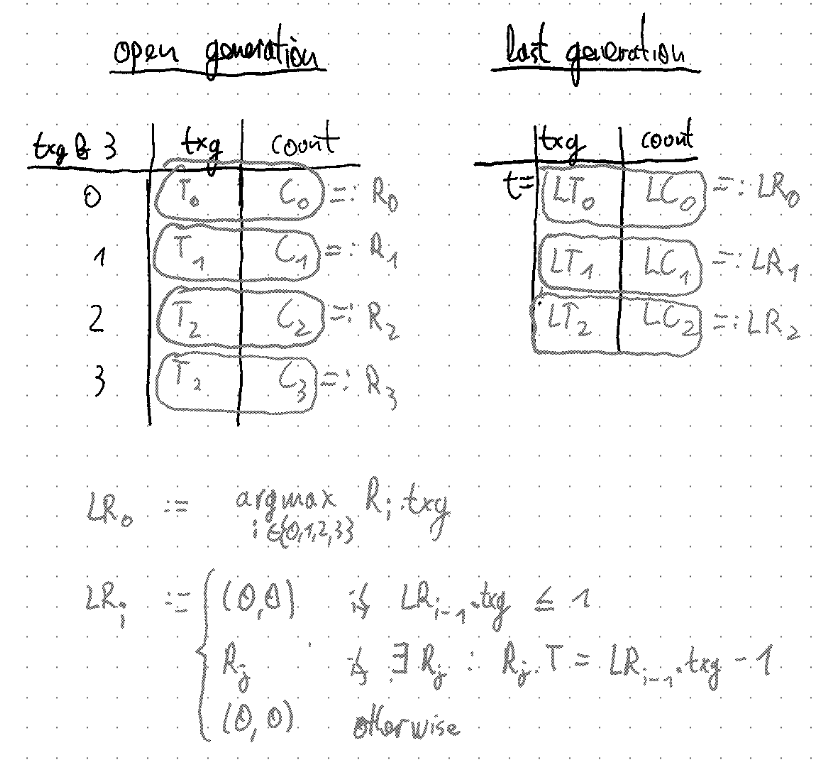
\includegraphics[width=\textwidth]{fig/prb_counters_table__computation}
    \caption{
        Visualization of the \textit{live} and \textit{last table} structures, and the algorithm used to compute the \textit{last table} from the \textit{live table} when a new generation is started.
        Note that we also provide an Example in Figure~\ref{fig:prb_counters_table__example}.
    }
    \label{fig:prb_counters_table__computation}
\end{figure}

\begin{figure}[H]
    \centering
    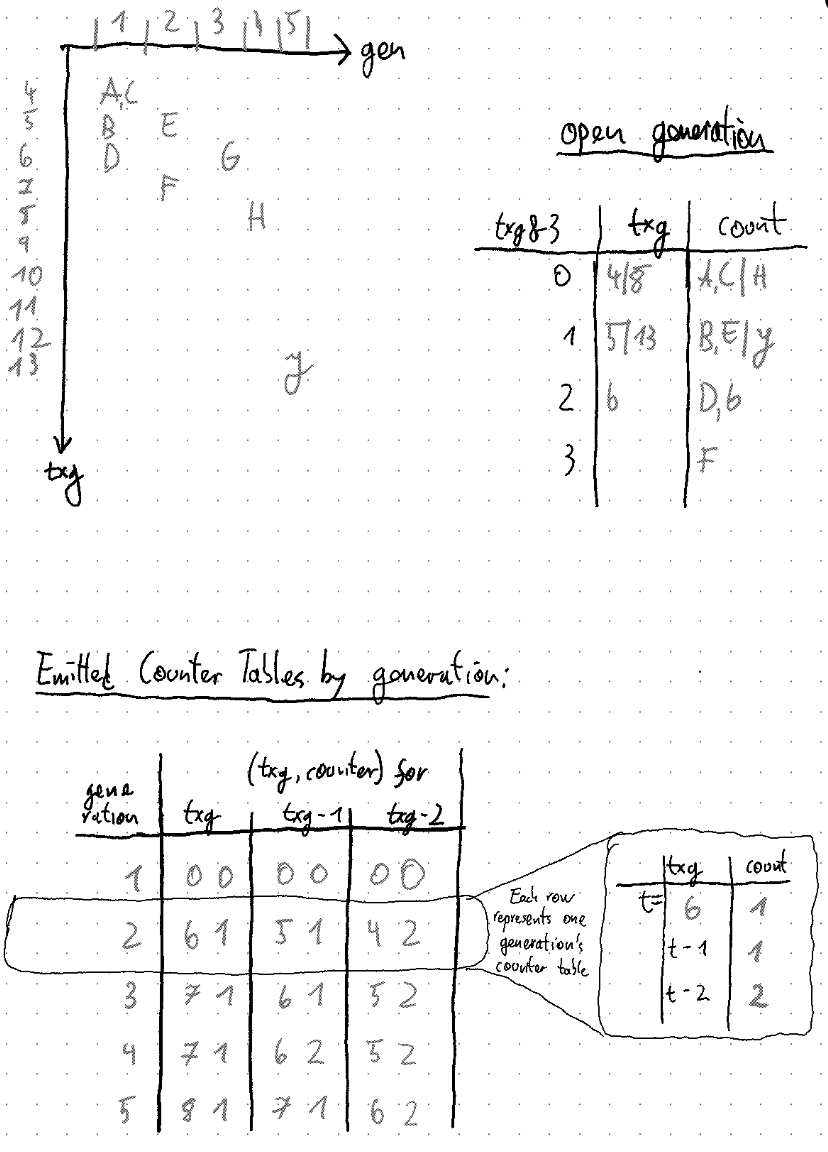
\includegraphics[width=\textwidth]{fig/prb_counters_table__example}
    \caption{
        Example for the computation of the Counter Table.
        The following entries are written to the log:
        A,B,C,D in generation 1; E,F in generation 2; G in generation 3; H in generation 4; J in generation 5.
        Note that their txgs differ some times but stay in the corridor of at most three a corridor of three txgs.
        The table at the bottom shows the Counter Tables in the entry headers:
        each row represents the counter table that is stored in the entry headers of one generation.
        The table at the upper right shows the \textit{live table} over time.
        Instead of counters, we show the entries that would cause the specific counter to be incremented.
        We visualize row-reuse by separating new row content with a "$|$" in each cell of the reused row.
    }
    \label{fig:prb_counters_table__example}
\end{figure}

% \begin{figure}
%     \centering
%     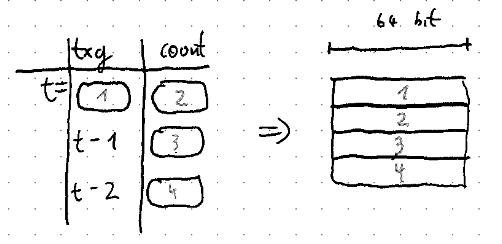
\includegraphics{fig/prb_counters_table__encoding}
% \end{figure}

\subsubsection{Crash-Consistent Append}\label{di:prb:write:crashconsistency}
After the target chunk and the entry metadata (Log GUID, txg, gen, gsid, Counters Table) have been determined, we are ready to append the entry to the sequence stored in the chunk.
In order to not lose log entries, the append operation must be crash-consistent with regards to the traversal algorithm (Section~\ref{di:prb:traversal}):
\begin{displayquote}
    Appending an entry $E_{n+1}$ to a chunk $C$ that contains a sequence of entries $E_1,~\dots,~E_n$ must be atomic from the perspective of traversal.
    After a system crash or power failure during the append operation, traversal of $C$ must either find $E_1,~\dots,~E_n$ or $E_1,~\dots,~E_n,~E_{n+1}$.
\end{displayquote}
The following algorithm describes the procedure and invariants during the append operation.
Figure~\ref{fig:prb_writepath_crashconsistent_append} contains a step-by-step visualization.
\begin{lstlisting}[style=figurepseudocode]
Inputs:
    ch  The chunk into which we append
    e   The entry that we append to ch's sequence.
Procedure:
  Invariant 1: Traversal will stop at ch.pos because
               either: ch.pos points to PMEM space that
                       is an invalid header
               or: there is no space left in the chunk

  Phase 1:
    Write e.body to address ch.pos + 256
    Write trailing zero padding
    If there is still space in the chunk at
      address ch.pos + 256 + e.body_len + padding_len:
        Assert that the space is at least 256 bytes.
        Write an invalid follow header (256 zero bytes)
          to that address.
    Cacheflush + Sfence

  Corrolary 1: Neither body nor follow header
               will be visited by traversal
               because traversal still stops
               at address ch.pos (Invariant 1).

  Phase 2:
    Write e.header (256 bytes) to address ch.pos
    Cacheflush + Sfence

  Corrolary 2: Traversal visits the entry written
               to ch.pos and stops at the follow
               header.
\end{lstlisting}
Invariant 1 can be proven by induction:
if the entry being written is the first entry in the sequence (base case) the chunk was fetched from the \textit{free list} which is defined to only contain chunks that are \textit{reset}.
(Section~\ref{prb:di:chunkownership}: \textit{reset} means that the write position (\lstinline{ch.pos}) is at the chunk's base address and that the PMEM at the write position is an invalid header.)
% The induction step is that if invariant 1 holds for a sequence with entries $E_1~\dots~E_n$, it also holds for a sequence with entries $E_1~\dots~E_{n+1}$.
The induction step is that if an entry $E_{n+1}$ is appended to an existing sequence $E_n$, invariant 1 holds as well.
This is true because the space occupied by $E_{n+1}$ contains an invalid follow header written by phase 1 when $E_n$ was appended to the sequence.
Stores made in Phase 1 for $E_n$ are guaranteed to be persistent before any store for $E_{n+1}$ happens due to the \lstinline{cacheflush+sfence} at the end of Phase 1.
Note that we do not need to address the case where the chunk is full because we cannot append $E_{n+1}$ to a full chunk.

The first \lstinline{sfence} (phase 1) is required for correctness if we trust the body checksum to detect partial writes instead.
If we omitted the \lstinline{sfence} in phase 1, it would be possible that the valid entry header written in phase 2 reaches PMEM completely but the body written in phase 1 does not.
In that case, after a crash, the traversal algorithm would observe a valid header with a body space with undefined content.
When the replayer loads the body using \lstinline{zilpmem_prb_replay_read_replay_node}, we would rely fully on failing body checksum validation to detect the partially written body.
If the checksum is too weak to detect the partial write, the replayer's interpretation of the undefined body contents determines subsequent behavior.

The \lstinline{sfence} (phase 2) is required for correctness  because we must conservatively assume that the log writer's subsequent store instructions (in program order) depend on the entry having reached stable storage.

\begin{figure}[H]
    \centering
    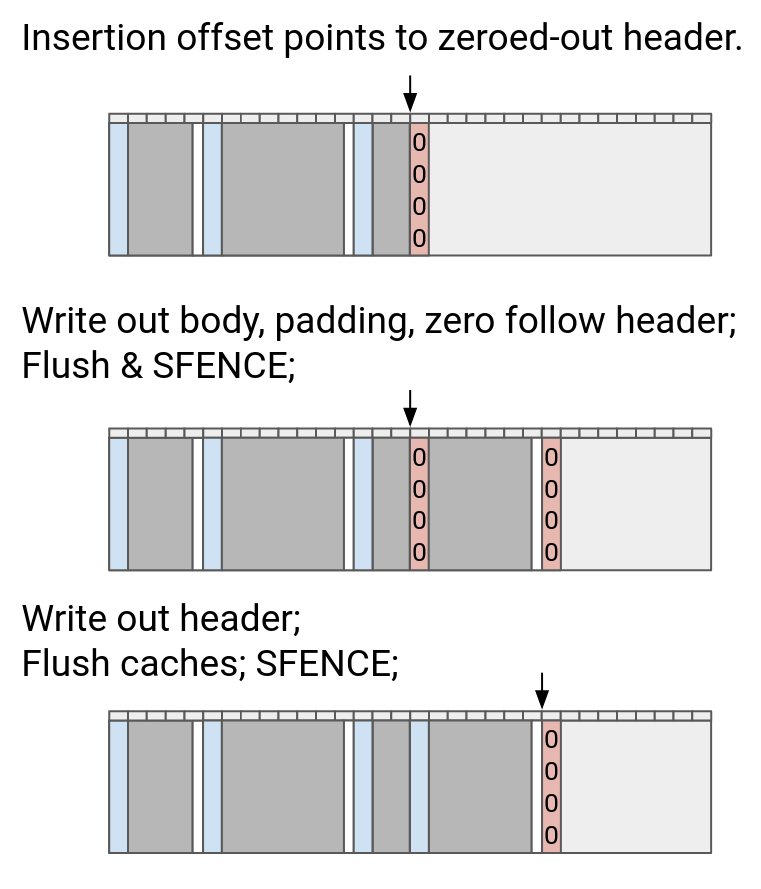
\includegraphics[height=6cm]{fig/prb_writepath_crashconsistent_append}
    \caption{
        The crash-consistent append operation to a PMEM chunk.
        The traversal algorithm reaches the existing entries at all times and reaches the new entry only after its body and header have been written completely.
    }
    \label{fig:prb_writepath_crashconsistent_append}
\end{figure}

The following aspects are relevant for latency and efficient use of CPU time:
\begin{itemize}[noitemsep]
    \item For ZIL-PMEM, the use of \lstinline{sfence} in phase 1 came with negligible impact on overall latency during development.\todo{need to prove this? don't have time...}
        We assume that this is because the wait time added by the \lstinline{sfence} is neglible compared to the write time for the entry body.
        For example, the entry body and zero padding for a 4k sync write is $sizeof(lr_write_t) + data + padding = 4096 + 192 + 64 = 4352$ bytes large.
        Assuming \SI{2}{GiB/s} write bandwidth for a single Optane DIMM (\cite{yangEmpiricalGuideBehavior2020}), the write time for the entry body is $\sim$~\SI{2}{us}.
        In contrast, the derived latency for a 256 byte write at that rate is $\sim$~\SI{0.12}{us}.
        If we use this value as an approximation for the cost of the \lstinline{sfence}, its latency contribution is only $\frac{0.12}{0.12 + 2} = 5.6\%$.
        Note that we have not systematically evaluated the effect.\todo{should we do this? if so, need also evaluate on different pmem configurations}
    \item All writes to PMEM happen in multiples of 256 bytes because 256 bytes is Optane's internal write unit size.
        Writes below this size cause read-modify-write cycles in the hardware and thus cost performance~\cite{yangEmpiricalGuideBehavior2020,zhangChameleonDBKeyvalueStore2021}.
    \item In the implementation we use AVX-512 non-temporal store instructions instead of \lstinline{write + cacheflush}.
        Again, this addresses established performance properties of Intel Optane DC Persistent Memory~\cite{yangEmpiricalGuideBehavior2020}.
\end{itemize}

\subsection{Recovery Path}\label{di:prb:recovery}
In this section we present how we recover log entries for unsynced transaction groups after a system crash.
Recovery is split into the \textit{claiming phase} and the \textit{replay phase}.
In the claiming phase during pool import, we discover which chunks need to be held back because they contain replayable log entries for at least one dataset.
In the replay phase, we apply the unsynced changes that are encoded in the entries of a particular log to its dataset.

\subsubsection{Replay Sequence Algorithm}
The basis for claiming and replay is the \textit{replay sequence algorithm}.
Its inputs are the HDL's log GUID, a set of \lstinline{prb_chunk_t} references, and a callback.
The algorithm consists of a \textit{scanning phase} and an \textit{iteration phase}.
The scanning phase uses the traversal algorithm (Section~\ref{di:prb:traversal}) to search for log entries that have the HDL's \textit{log GUID} in all chunks that are provided as input.
It wraps each of these candidate entries in a \textit{replay node} and collects the nodes in a b-tree.
In the \textit{iteration phase}, the algorithm \textit{visits} each replay node by iterating over the b-tree.
For each node, it checks whether the corresponding entry still needs to be replayed and if so, invokes the provided callback.
It detects missing entries on-the-fly before invoking the callback.

The \textit{replay node} stores the following metadata about an entry:
\begin{description}[noitemsep,leftmargin=1.5cm,labelindent=1cm]
    \item[Generation (gen)] The entry's generation.
    \item[Generation-Scoped ID (gsid)] The entry's generation-scoped ID.
    \item[PMEM Address] The start address of the entry in PMEM.
    \item[Transaction Group (txg)] The entry's transaction group.
    \item[Counter Table] The counter table stored in the entry.
    \item[Pointer To Chunk (chunk\_ref)] A pointer to the \lstinline{prb_chunk_t} that contains the entry.
\end{description}
The replay nodes of a well-formed HDL log are uniquely identified by $(gen, gsid)$.
%The b-tree identifies and sorts replay nodes by $(gen, gsid)$ in element-wise ascending order.
The lexicographical ordering of that tuple is the replay ordering, and also the ordering used in the b-tree.
For example, the replay nodes $(2,1), (1,1), (1,3)$ are visisted in order $(1,1), (1,3), (2,1)$.

\begin{samepage}
In the iteration phase, the algorithm visits each entry in the b-tree in the order defined above.
It uses the following state to evaluate the subsequently listed steps for each visited replay node $N$.
 \begin{description}[noitemsep,leftmargin=1.5cm,labelindent=1cm]
    \item[precrash-txg] The last transaction group that finished syncing before the system crashed.
    \item[$\mathbf{(gen_{last}, gsid_{last})}$] The $gen$ and $gsid$ of the last replay node that was visited.
        A value of $(0,0)$ means that no replay node has been visited yet.
    \item[validating counter tables] A \textit{live} and \textit{last} table; same layout as used on the write path (see Section~\ref{di:prb:write:logstructureencoding}).
\end{description}
% The following rules determine whether the callback is invoked for a replay node $N$:
% Remember that $E$ for generation $E.gen$ depends on all entries in all generations $gen < E.gen$.
% Also remember that $E$ must only be replayed if the changes of its transaction group $E.txg$ have not been applied to the dataset.
Steps per node $N$:
\begin{enumerate}[noitemsep]
    \item \label{replayStep:skiptxg} Skip $N$ if its $N.txg \le precrash\text{-}txg$.
    \item \label{replayStep:skipreplayed} $N$ if $(N.gen,N.gsid) \le (gen_{last}, gsid_{last})$.
    \item \label{replayStep:validate} Compare the validating \textit{last table}'s counters to the Counters Table stored in $N$.
        Only counters for $txg > precrash\text{-}txg$ must be compared because we skip entries for $txg \le precrash\text{-}txg$.
        Proceed iff the counters match. Otherwise, stop the iteration, and return $N$ as a witness for log corruption.
    \item \label{replayStep:bump1} If $N.gen \neq gen_{last}$, compute a new validating \textit{last table} from the validating \textit{live table}.
    \item \label{replayStep:bump2} Increment the validating \textit{live table}'s counter for txg $N.txg$.
    \item \label{replayStep:bump3} Update $(gen_{last}, gsid_{last}) = (N.gen, N.gsid)$.
    \item \label{replayStep:invoke} Invoke the callback provided by the algorithm's consumer, passing $N$ and the iteration state as arguments.
        If the callback returns an error, rollback the update to $(gen_{last}, gsid_{last})$ and the counter tables, stop the iteration, and return.
        Otherwise, proceed to the next replay node.
\end{enumerate}
\end{samepage}

The rationale behind these steps is as follows.
Step~\ref{replayStep:skiptxg} filters out entries whose changes had already been synced to the pool before the system crashed.
Step~\ref{replayStep:skipreplayed} filters out entries for which the callback has already been invoked.
Comparing the counters in step~\ref{replayStep:validate} ensures that we have already invoked the callback for all entries in generations $gen < N.gen$.
The subsequent steps \ref{replayStep:bump1}, \ref{replayStep:bump2}, and \ref{replayStep:bump3} record that the callback has been invoked for $N$.
Specifically, steps~\ref{replayStep:bump1} and \ref{replayStep:bump2} ensure that entries $(gen, gsid) > (N.gen, _)$ pass step \ref{replayStep:validate} as well.
And \ref{replayStep:bump3} ensures that $N$ is going to be skipped by step~\ref{replayStep:skipreplayed} in the future.

We externalize the iteration phase's state into a structure called \lstinline{zilpmem_replay_state_t}.
structureto achieve crash consistent replay.
Since replay happens during normal pool operation, it is not atomic because the replayed changes are spread over multiple transaction groups.
And since replay is also not idempotent, replay after a system crash must resume exactly after the last-synced replay node.


at the last-synced replay  rereplay exactly at the replay node before  must not we cannot retry replay from the beginning of the log either.must not replay entries that have already been replayed.



since 
the replay callback serializes the iteration phase's state in the \lstinline{zilpmem_replay_state_phys_t} structure that is stored in the ZIL header (Section~\ref{di:prb:persistent:zilheader}).
If the system crashes during replay, we cannot restart from the beginning because ZIL replay is not idempotent.
Instead, we must resume exactly where the last 


Our solution is to externalize all of the iteration phase's state into the \lstinline{zilpmem_replay_state_t} structure.
The \lstinline{zilpmem_replay_state_t} is the dirty in-DRAM copy of the on-disk \lstinline{zilpmem_replay_state_phys_t} which is stored in the ZIL header (Section~\ref{di:prb:persistent:zilheader}).
It is the responsibility of claiming and replay to keep the two in sync.
After a system crash during claiming or replay, the HDL setup routine recovers the in-DRAM state from the last-synced on-disk state in the ZIL header.
The replay sequence algorithm is thus unaware of the crash.

This is necessary when the algorithm is used by replay: the callback provided by replay persists the iteration phase's state to the ZIL header.

% The callback invoked in \ref{replayStep:invoke} thus 
% The callback invocation in \ref{replayStep:invoke} is then supposed 
% Step~\ref{replayStep:bump3} ensures that $N$ will not be replayed a second time if we restart the iteration.
% We have to apply the state updates of steps \ref{replayStep:bump1}, \ref{replayStep:bump2}, and \ref{replayStep:bump3} \textit{before} invoking the callback in Step~\ref{replayStep5} because the replay persists the iteration state.
% Thus if the callback indicates failure, we must roll back the updates so that
% If the update fails,  If the callback fails, we therefore need therefure need that we have not lost all previous ~and~\ref{replayStep3b} count the number of entries that werwewre-enact 

% Entries  from before the We must replay entries whose change must skip steps We skip  that have alread The logic behind step~\ref{stepValidatingCountersTables} is that 

A number of critical properties of the overall algorithm result from this counter validation step:
\begin{enumerate}[noitemsep]
    \item It is guaranteed that the witness $(gen_w, gsid_w)$ for a lost entry $(gen_l, gsid_l)$ is always the first entry in the b-tree whose $gen_w > gen_l$.
    \item Thus, all other found entries $(gen_l,  \_)$ in a generation with a lost entry are still replayed before the error is detected and iteration stops.
    This is correct and desirable because by definition, entries within a generation have no logical dependency on each other.
    \item Loss of entries at the tail of the logical log cannot be detected because there is no record of their existence in prior log entries.
    Note that this is the status quo with ZIL-LWB as well, both with and without OpenZFS Native Encryption.
\end{enumerate}
We provide examples for counter table validation in Figure~\ref{todo}.

The correctness of the replay sequence algorithm relies on the assumption that random data corruption is incapable of ``forging'' new log entries that would appear in the b-tree.
If a forged entry appears, the behavior depends on the callback implementation --- interpretation of the forged log entry by replay may corrupt the dataset.
All of the following properties need to be fulfilled by an entry to affect the replay sequence algorithm:
\begin{itemize}[noitemsep]
    \item It has been correctly appended to a chunk's sequence as described in Section~\ref{di:prb:write:crashconsistency}.
    \item Its \textit{log GUID} matches the log in which it appears.
    \item Its \textit{txg} is in one of the unsynced txgs.
    \item Its $(gen, gsid)$ does not collide with the original entries that are collected in the b-tree.
\end{itemize}
We believe that it is sufficiently unlikely for random data corruption to produce an entry that fulfills all of these properties.
Apart from random data corruption, we have considered the following scenarios:
\begin{itemize}[noitemsep]
\item Implementation errors on the write path or in the traversal algorithm.
\item Firmware bugs, e.g., in the Optane DIMM's wear-leveling layers, that could make old entries re-appear.
\item Deliberate injection of log entries by a malicious party with write access to PMEM.
    We cannot protect unencrypted datasets from this kind of thread.
    But it must be part of the threat model for datasets encrypted using OpenZFS Native Encryption.
    While encryption support is out of scope for this thesis, forged entries should be detectable by authenticating the entry header.
\item Accidental reuse of \textit{log GUIDs}.
    If two HDLs use the same log GUID to write their entries, replay will collect both logs' entries in the same b-tree.
    This scenario is very unlikely because we generate log GUIDs as 128 bit random numbers.
    The b-tree allows us to detect some cases of log GUID collisions during the scanning phase when we attempt to insert an entry with a duplicate $(gen, gsid)$.
    In that case, we abort execution of the the algorithm immediately with an error.
    However, we would prefer a more comprehensive approach to systematically prevent log GUID reuse.
    \todo{impl currently does this, but I thought about this during writing and it's not a good idea}
    \todo{future work section on log guid reuse, see latex comment here}
\end{itemize}
% Future work could mitigate the risk of log GUID collision in PMEM as follows:
%  1. Maintain a hashset of active log guids, let's call id H_a.
%  2. Newly issued log guids must not be in H_a but are added to it once they are issued.
%  3. During pool import, traverse all chunks and add all guids that are found to H_a.
% This covers most scenarios except if new entries can 'appear' in the future, e.g. due to weird storage firmware bugs, etc.
% Note that a pool-wide sequence number for log GUIDs does not fix the issue because it would be rolled back if zpool checkpoints are used.\todo{ref ZIL-PMEM?}
% We should think about whether we can store the sequence number in PMEM which is not rolled back, but that opens up a whole other can of worms...

%\item If any of the checked counters in the validating \textit{last table} are lower than the corresponding counter in $E$'s Counters Table, we know that we have lost entries.
%In that case, we do not invoke the callback and return an error which contains $E$ as a witness.
%\item If any of the checked counters in the validating \textit{last table} are greater than the corresponding counter in $E$'s Counters Table, we have a witness for a structurally corrupted log and stop iteration.
%Note that we might already have invoked the callback for several log entries before noticing this kind of corruption.
%We cannot protect against the scenarios that lead to it:
%\begin{itemize}
%    \item The witness is false (data corruption of $E$'s Counters Table undetected by the header checksum).
%    \item An entry appeared that was never written (malicious intent, firmware bugs).
%    \item Implementation error on the write path.
%\end{itemize}
%\end{enumerate}

The replay sequence algorithm is resilient against random \textit{online} data corruption in PMEM, i.e., data corruption while the algorithm executes.
The reason is that both phases only operate on DRAM-buffered copies of the entry metadata in the replay node.
Further, if the callback needs to read the entry, our API forces it to use DRAM-buffering as well:
it does not receive a pointer into PMEM but a pointer to the (opaque) replay node struct.
To copy the entry into a DRAM buffer, it must use the \lstinline{zilpmem_prb_replay_read_replay_node} function which
\begin{itemize}[noitemsep]
    \item handles machine-check exceptions (MCEs) through \lstinline{memcpy_mcsafe},
    \item validates the header and body checksums of the entry, and
    \item ensures that the metadata cached in the replay node did not change since the scanning phase.
\end{itemize}


\subsubsection{Claiming}
The claiming phase during pool import (\lstinline{zilpmem_prb_claim}) uses the replay sequence to find the set of chunks that contain entries of the log that is being claimed.
This set of chunks is stored in DRAM inside the HDL for later use by replay.
We refer to it as the HDL's \textit{claimset}.

The set of chunks that claiming provides as input to the algorithm are the chunks on the \textit{wait replay list} which was filled by \lstinline{zilpmem_prb_add_chunk_for_claim} during PRB construction (Section~\ref{prb:di:chunkownership}).
The callback performs the following steps for each replay node $N$ for which it is invoked:
\begin{enumerate}
    \item Add the chunk $N.chunk\_ref$ to the HDL's claimset.
        If the chunk was not yet included in the set, increment the chunk's \textit{claim refcount} (Section~\ref{prb:di:chunkownership}).
    \item Check for PMEM corruption by reading the log entry from PMEM using \lstinline{zilpmem_prb_replay_read_replay_node}.
\end{enumerate}
If log corruption is detected by the replay sequence algorithm or the callback, we fail the pool import operation.
In that case, the \textit{claim refcount}s are decremented during HDL teardown.
\todo{in the impl, we currently panic on error because we'd need to change how import works. It's just a bunch of engineering work, not relevant for the thesis.}
Otherwise, if no errors have occured, the HDL transitions into a state where it waits for replay.

Note that claiming invokes the replay sequence algorithm with a throw-away in-DRAM copy of the replay state because no actual replay is happening in the callback.
However, claiming is responsible for transitioning the ZIL header from \textit{logging} to \textit{replaying} when the log is first claimed after a crash.
During this transition, it initializes the \lstinline{zilpmem_replay_state_phys_t} associated with the \textit{replaying} state.
The value for $precrash\text{-}txg$ is the pool's first transaction group that will be synced once txg sync starts.
$(gen_{last}, gsid_{last})$ is $(0, 0)$.
All rows in the \textit{validating counter tables} are invalidated by setting their $txg$ to $0$.

\subsubsection{Replay}
% reconstructs replay sequence, only scans HDL's held chunks list
% explain how replay stores its state in a struct
% state is serialized and passed replay callback for DMU transaction
% explain how crash during replay and resume works
Replay (\lstinline{zilpmem_prb_replay}) uses the replay sequence algorithm to recover dataset state.
Remember from Section~\ref{di:prb:api:replay} that \lstinline{zilpmem_prb_replay} itself receives a callback $C_{consumer}$ from the API consumer.
The API contract states that $C_{consumer}$ receives the replay node and an updated version of the ZIL header as arguments.
It must, in one DMU transaction, replay the change encoded in the replay node's entry and apply the ZIL header update.
This makes \lstinline{zilpmem_prb_replay} is a thin wrapper around the replay sequence algorithm.
The set of chunks to be traversed by the algorithm is the \textit{claimset} that the claiming procedure stored in the HDL.
A thin wrapper callback $C_{wrapper}$ translates from the replay sequence algorithm's limited view on replay to the HDL-wide view of the replay API.
$C_{wrapper}$ receives the replay node $N$ as an argument. It performs the following steps:
\begin{enumerate}
    \item Compute the new ZIL header $H_{new}$ from the HDL state.
        The replay sequence algorithm already updated the replay state before invoking the callback, thus $H_{new}$ will contain the updated \lstinline{zilpmem_replay_state_phys_t}.
    \item Invoke $C_{consumer}(N, H_{new})$ and return its return value.
\end{enumerate}

\section{ZIL-PMEM}\label{sec:zilpmem}
In this section we describe how we use PRB/HDL to implement ZIL-PMEM as a new ZIL kind.

\section{ITXG Bypass For ZVOL}\label{sec:itxgbypass}
In this section we describe a performance optimization for ZIL-PMEM that allows for parallel log writes to a single ZVOL.



\begin{lstlisting}
    typedef struct zilpmem_replay_state_phys {
        uint64_t claim_txg;
        eh_dep_t resume_state_active;
        eh_dep_t resume_state_last;
    } zilpmem_replay_state_phys_t;
    
    typedef struct eh_dep {
        uint64_t eh_last_gen;
        prb_deptrack_count_pair_t eh_last_gen_counts[TXG_CONCURRENT_STATES];
    } eh_dep_t;
    
    typedef struct prb_deptrack_txg_seq_pair {
        uint64_t dtp_txg;	/* 0 <=> invalid pair */
        uint64_t dtp_count;	/* 0 <=> invalid pair */
    } prb_deptrack_count_pair_t;
    \end{lstlisting}
    

\chapter{Evaluation}\label{ch:eval}
\section{Correctness}
We evaluate the correctness of our work through unit and integration tests.
\subsection{PRB}
\subsection{ZIL-PMEM}
\section{Performance}
We evaluate the performance of ZIL-PMEM with a variety I/O benchmarks.
\subsection{Write Performance}
\subsubsection{4k Random Sync Writes}
\subsubsection{Application Benchmarks}
\subsection{Replay Performance}

\chapter{Related Work}

\backmatter

\chapter{Appendix}\label{ch:appendix}

\cleardoublepage
\phantomsection
\addcontentsline{toc}{chapter}{Bibliography}
\emergencystretch=1em
\printbibliography

\end{document}
